% use option [draft] for initial submission
%            [final] for the prepublication
\documentclass[ecta,nameyear,draft]{econsocart}
%\documentclass[]{econsocart}
%
%\usepackage{}
\RequirePackage[colorlinks,citecolor=blue,linkcolor=blue,urlcolor=blue,pagebackref]{hyperref}

\startlocaldefs

\usepackage{booktabs}
\usepackage{multirow}
\usepackage{float}         
\usepackage{amsmath}
\usepackage{amscd}
\usepackage{amsfonts}
\usepackage{amssymb}
\usepackage{bbm}
\usepackage{dsfont}
\usepackage{colortbl}
\usepackage{comment}
\usepackage{lscape}
\usepackage{subcaption}
\newtheorem{theorem}{Theorem}
\newtheorem{claim}[theorem]{Claim}
\newtheorem{prop}[theorem]{Proposition} 
\newtheorem{cor}[theorem]{Corollary} 
\newtheorem{assumption}{Assumption} 
\newtheorem{lem}{Lemma} 
\usepackage{enumerate}

\newcommand{\wh}{\widehat}

\newcommand{\E}{\mathbb{E}}

\endlocaldefs

\usepackage[section]{placeins}

\begin{document}


\begin{frontmatter}

\title{The controlled choice design and private paternalism in pawnshop borrowing}
\runtitle{The controlled choice design and private paternalism}

\begin{aug}
% use \particle for den|der|de|van|von (only lc!)
% [id=?,addressref=?,corref]{\fnms{}~\snm{}\ead[label=e?]{}\thanksref{}}
%
%% e-mail is mandatory for each author
%
%%% initials in fnms (if any) with spaces
%
\author[id=au1,addressref={add1}]{\fnms{Craig}~\snm{McIntosh}\ead[label=e1]{ctmcintosh@ucsd.edu}}
\author[id=au2,addressref={add2}]{\fnms{Isaac}~\snm{Meza}\ead[label=e2]{isaacmezalopez@g.harvard.edu}}
\author[id=au3,addressref={add3}]{\fnms{Joyce}~\snm{Sadka}\ead[label=e3]{jsadka@itam.mx}}
\author[id=au4,addressref={add4}]{\fnms{Enrique}~\snm{Seira}\ead[label=e4]{enrique.seira@gmail.com}}
\author[id=au5,addressref={add5}]{\fnms{Francis J.}~\snm{DiTraglia}\ead[label=e5]{francis.ditraglia@economics.ox.ac.uk}}

% Addresses
\address[id=add1]{%
\orgdiv{Department of Economics}
\orgname{University of California San Diego}}

\address[id=add2]{%
\orgdiv{Department of Economics}
\orgname{Harvard University}}

\address[id=add3]{%
\orgdiv{Department of Economics}
\orgname{Instituto Tecnologico Autonomo de Mexico}}

\address[id=add4]{%
\orgdiv{Department of Economics}
\orgname{Michigan State University}}

\address[id=add5]{%
\orgdiv{Department of Economics}
\orgname{University of Oxford}}
\end{aug}

%% Put support info here. Reminder: do not thank the handling coeditor anonymously or by name
\support{We want to thank Mauricio Romero and Anett John for advice and encouragement. Ricardo Olivares, Gerardo Melendez, and Alonso de Gortari provided excellent research assistance and Erick Molina helped with formatting. Jose Maria Barrero, Andrei Gomberg, Emilio Gutierrez, David Laibson, Aprajit Mahajan, Matt Rabin, Charlie Sprenger, and seminar participants at ITAM, USC, MSU, and UCSD provided valuable feedback. Research assistance was financed through faculty grants at ITAM. Our research partner had no say in the results.}
%
\coeditor{\fnm{[Name} \snm{Surname}; will be inserted later]}

\begin{abstract}
We use a novel three-armed RCT, including both forced and voluntary treatment arms, to provide a unique window into choice, heterogeneous treatment effects and paternalism in the context of pawnbroker lending. Forcing borrowers into commitment contracts with a regular repayment structure decreases the financial cost of pawn loans by 22\% inclusive of fees, increases the likelihood of recovering their pawn by 15\%, and increases the likelihood of repeat business by 19\%. Leveraging the special features of our experimental design, we go on to point-identify the effects of commitment on both the treated and the untreated simultaneously, along with the average selection on gains. We find large and significant effects of commitment even for borrowers who would not voluntarily choose it, and no evidence of selection on gains: borrowers who would freely choose commitment do not appear to benefit more than borrowers who would not. A detailed analysis of treatment effect heterogeneity suggests that the potential gains from targeting commitment based on observable characteristics are extremely small and that most borrowers stand to gain from a policy of universal forced commitment.
\end{abstract}


\begin{keyword}
\kwd{Private paternalism}
\kwd{choice}
\kwd{treatment on the untreated}
\kwd{heterogeneous treatment effects}
\kwd{commitment}
\kwd{overconfidence}
\end{keyword}

\end{frontmatter}
%%%%%%%%%%%%%%%%%%%%%%%%%%%%%%%%%%%%%%%%%%%%%%%%%%%%%%%%%%%%%%%%%%%%%%%%%
%%%% Main text entry area:
%%%%%%%%%%%%%%%%%%%%%%%%%%%%%%%%%%%%%%%%%%%%%%%%%%%%%%%%%%%%%%%%%%%%%%%%%


\section{Introduction}

The behavioral finance literature has established an important role for commitment devices in helping consumers to achieve their own financial goals.  While most academic studies on commitment focus on the role of voluntary self-commitment \citep{thaler2004save, prina2015banking, brune2016facilitating, callen2019headwaters, Pascaline, Ashraf}, in reality the predominant use of rigid structure in financial services is involuntary; firms only offer a product with these features embedded.  \cite{Laibson2018} has referred to this implicit bundling of commitment devices as ``private paternalism'', and its logic is that individuals may benefit from commitment and yet not explicitly demand it.  Comparing voluntary versus paternalistic programs requires that we form counterfactuals for two different groups of people: those who would freely choose commitment, and those who would not (since the latter group is treated only under paternalist policies). In this paper we present an experimental design and econometric analysis that point-identifies and provides estimates for both the effect of treatment on the treated (TOT) and on the untreated (TUT). This permits a clear window into the case for paternalistic (forced) rather than voluntary commitment in financial services.

The relationship between treatment effects and treatment take-up is a core concern in the econometrics literature. In principle, the Marginal Treatment Effect (MTE) approach allows researchers to use observational data and a single excluded instrument to study this relationship. In practice, however, unless the instrument has a rich support set, MTEs can only be point identified by using additional modeling assumptions \citep{mogstad2018using}. An alternative research strategy to study the relation between treatment effects and treatment take-up uses the Becker-Degroot-Marschak (BDM) mechanism, incentivizing choice prior to treatment assignment to elicit willingness to pay (WTP) for treatment \citep{becker1964measuring}. 
A number of studies, however, find that the WTP elicited under the BDM mechanism changes substantially with the distribution of prices used in the elicitation exercise \citep{bohm1997eliciting,banerji2014detection}. This falsifies the assumption of standard preferences that is required for BDM to be incentive-compatible \cite{mamadehussene2023reliability}, suggesting that the mechanism may not provide a reliable measure of actual compliance  in practice.
Our study avoids the drawbacks of the MTE and BDM approaches by combining a novel three-armed randomized controlled experiment, including forced treatment and treatment choice arms, with two transparent exclusion restrictions. Together, these allow us to point identify the relevant TOT and TUT effects in a real-world, high-stakes setting and to study the case for paternalistic commitment head-on, with minimal assumptions.

We apply this approach to an important and understudied context: pawnshop lending. 
Pawn loans constitute one of the oldest and most prevalent forms of borrowing \citep{carter2012pawnshops}.
Our partner lender, for example, made over 4 million loans to more than a million clients during the past three years.\footnote{For comparison, there were 2.3 million microfinance clients in Mexico in 2009 \citep{Pedroza:2010}.} 
The question of choice versus paternalism is particularly salient in this context, as choice mistakes could arise from borrowers' low education and the fact that they typically borrow for emergencies under significant stress.\footnote{A large literature shows  stress impairs cognitive function, e.g. \cite{StressReview}.}
%\footnote{There are more than 11,000 pawn shops across the US, with 30 million clients and \$14 billion yearly revenues (in China it is a \$43 billion industry).  \url{https://tinyurl.com/ybm56dpe}, \url{https://tinyurl.com/y9zdcgws}, \url{https://tinyurl.com/y59ptdam}.}
Our experiment covers just under 5,000 pawnshop clients in 6 of our partner lender's Mexico City branches. Our control arm illustrates the costs of the status quo contract: fully \emph{44\%} of borrowers default, losing lose their pawn along with any payments made towards principal.\footnote{High pawn default rates are common, in the US they oscillate around 15\% (see \href{https://tinyurl.com/yc2x5bjf}{here}).} Our ``commitment choice'' arm gives borrowers the chance to opt into a structured repayment contract when taking a loan. The structured contract requires borrowers to make three monthly payments rather than one balloon payment at the end, with each monthly payment including the accrued interest at that time as well as a nominal fee of 2\% of that month's payment if the payment is delinquent. The fee serves as a reminder and a means of reinforcing the importance of these interim payments. In our ``forced commitment'' arm all borrowers are \emph{required} to repay using the same structured monthly contract offered on an opt-in basis in the commitment choice arm. 

%The combination of voluntary and forced commitment within the RCT allows us to address several key questions. 
We address three key questions. First, do structured repayment contracts lower financial costs for pawnshop borrowers? Second, do borrowers recognize this benefit, demanding commitment in sufficient numbers?  Finally, and most uniquely, do the \textit{right} borrowers voluntarily demand commitment? Our ability to answer the last question comes from our unique three-armed experimental design, which we call the ``controlled choice design'' for short. This design can be viewed as a juxtaposition of \emph{two} randomized encouragement designs, each with one-sided non-compliance. One of them point identifies the effect of commitment for borrowers who would \emph{voluntarily} choose commitment (TOT),
while the other point identifies the effect of commitment for borrowers who would \emph{not} (TUT).
By identifying both the TOT and TUT effects in the same experiment, the controlled choice design allows us to examine the empirical relevance of ``selection on gains'' also known as Roy-type selection into treatment by estimating the ``average selection on gains'' $\text{ASG} = \text{TOT} - \text{TUT}$. This enables us to test whether borrowers who voluntarily choose commitment have higher average treatment effects than those who do not, rather than assuming it. The controlled choice design also point identifies the average selection bias (ASB)--the average difference in untreated (status quo) potential outcomes for those who choose commitment relative to those who do not--along with the average selection on levels (ASL)--the analogous comparison for treated (commitment) potential outcomes. Taken together, these causal effects allow us to ``go under the hood'' of our baseline ATE results, and paint a more complete and economically relevant picture of the effects of commitment. We are unaware of any other paper that simultaneously identifies all of these causal effects without recourse to additional structural modeling assumptions. 

We find that commitment is strongly effective in lowering financial costs and preventing default in pawnshop lending: the average individual in the forced arm pays financing costs inclusive of fees that are 22\% lower than the control, and faces a probability of default that is 6.6 percentage points lower (15\% of the mean). In terms of Annual Percentage Rates, the financial cost of borrowing falls by 11 percentage points (19\% of the mean). In short, structured commitment saves borrowers money by charging them fees! Our results are qualitatively robust to deducting transport costs of visiting the branch to make interim payments along with a day of lost wages for each visit. They are also robust to using borrowers' \emph{subjective} values of their pawns rather than the appraised value of the gold, and to adjusting for lost liquidity from requiring monthly payments.  The monthly payment contract seems to achieve these cost savings by speeding up payments and by generating an early bifurcation of borrowers into those that will recover the pawn and those that will not. The former are induced to pay faster, saving on interest; the latter pay less towards loans that ultimately default, hence losing less money when they do. 

Despite these large financial cost savings, only 11\% of borrowers in the choice arm choose commitment. 
%If the effect of commitment were homogeneous, this would be enough to conclude that the 89\% who did not choose it would have been financially better off if they had. However, we test and reject the null hypothesis of homogeneous treatment effects using the method of \cite{chernozhukov2018generic}. 
Can the borrowers who did not choose commitment be those who simply don't need it? 
To answer this question, we carry out a detailed analysis of treatment effect heterogeneity.
%We address this question by sequentially imposing more structure on the problem. 
We begin by bounding the distribution of individual treatment effects using the marginal outcome distributions from the forced commitment and control arms, following \cite{fan2010sharp}. This approach imposes no assumptions beyond the experimental randomization. We find that \textit{at least} 23\% of borrowers benefit from commitment. This implies that there must be many borrowers in the choice arm who did not demand commitment despite their \emph{individual treatment effect} from (forced) commitment being positive. Next, we impose an exclusion restriction positing that the effect of a given contract does not depend on \emph{how} borrowers obtain it. In other words, we assume that choosing a contract results in the same potential outcome as being assigned that contract. This is a relatively common if often implicit assumption in causal inference.\footnote{Papers that use variation in compulsory schooling laws to identify the returns to schooling, for example, typically interpret their results as the causal effect of additional \emph{education} rather than additional \emph{forced education}. \cite{chamberlain2011bayesian} uses a closely related assumption to develop a theory of optimal treatment choice.} 
It also has testable implications that we fail to reject in our empirical context.\footnote{See \autoref{sec:testing_exclusion} for details.}
Under this restriction, the controlled choice design point identifies the TOT, TUT, ASG, ASB, and ASL effects described above.  Our estimated TUT effect on financial cost savings is large: \$192 pesos, equivalent to a 10.6 percentage point savings in APR. On average, the borrowers who would \textit{not} choose commitment, would have faced substantially lower financial costs if they had. Finally, we combine our experimental treatment and outcome data with survey responses collected for a subset of borrowers to estimate conditional average treatment effects, both TUTs and ATE, using the Causal Random Forest algorithm of \cite{atheygrf}. We estimate positive conditional average TUT effects for 93\% of the borrowers who did \textit{not} choose the commitment contract. 
In short, it is extremely difficult to find identifiable groups of borrowers who are \emph{harmed} by commitment, even when restricting attention to those who would not choose it voluntarily. 
%while only 37\% of those who chose commitment have negative conditional TOT effects.
While targeting commitment products to those that benefit the most is a policy that appears attractive, in this context we find that the usable targeting variables have relatively weak predictive power and hence even our best random forest targeting only reduces the overall mis-targeting rate from 9.7\% (all to Forcing) to 9.5\% (our best-case feasible targeting mechanism).

What explains the persistence of no-commitment contracts so contrary to borrowers’ interests in the real world?  From the demand side, while a simple measure of time inconsistency does not explain the large and positive TUT effect, we show substantial levels of over-optimism among borrowers. Among borrowers who do not choose commitment, those with the largest estimated benefits from commitment are the individuals who most systematically over-estimate their own probability of repayment without the need to commit, potentially decreasing their demand from commitment. From the supply side, because borrowers' financial savings come directly from the pockets of lenders, pawnshops have an interest in retaining the no-commitment contract.
Indeed, pawnshop lending presents an inverted lending case: since these loans are over-collateralized, the lender in the contract stands to gain the most when borrowers default.  Our partner's \emph{status quo} pawn contract gave 70\% of the value of gold collateral in credit, and charged a monthly interest rate of 7\% for loans of a three-month duration, with a flexible no-reminders contract, that could be paid back anytime before the loan comes due at no penalty. This contract is standard contract in the industry. This combination of features, and the fact that the gold pawn is highly liquid, means that the lender makes 90\% more profit over three months from a borrower who defaults than one who repays (30\% of collateral value recovered under default, 15.8\% of collateral value paid in interest if loan fully repaid). While an older literature considers the exploitative potential of over-collateralization and underpriced collateral \citep{basu1984implicit}, the implication of such contracts has not been analyzed in the behavioral literature. 

%By overcollateralizing and then structuring loan contracts in a manner encouraging of default, lenders are able to extract substantial value independent of the interest charged.  

Our paper makes a number of contributions to the literature. First, we propose a way to use this three-armed experimental structure to recover treatment effects for choosers and non-choosers under minimal assumptions.\footnote{While \cite{fowlie2021default} likewise employ a three-armed experimental design in their study of the effect of electricity pricing, they identified \emph{two} TOT effects for different groups of ``treated'' households, whereas we simultaneously identify the TOT and TUT effects defined with respect to a single ``treated'' group of borrowers. This difference is what allows our design to point identify the ASG and related quantities.} 
A companion STATA package provides simple, regression-based estimators for each of these causal parameters, along with appropriate cluster-robust standard errors.\footnote{See \autoref{sec:estimation_inference} for details.} 
The controlled choice design could be useful in other experimental settings where the question of interest centers on the merits of paternalism, public or private, or the relationship between choice and treatment effects. One obvious example is the design of other financial contracts beyond pawn loans. Another is education, where teachers typically mandate quizzes, homework, and other commitment mechanisms to mitigate student procrastination \citep{Ariely}. 
We further contribute to a relatively small existing literature that sheds light on private paternalism. In the context of food choice, \cite{Sprenger} show that individuals with the most time-inconsistent preferences are actually least likely to demand commitment. In contrast to their paper, we directly identify the TUT, obviating the need to first elicit preferences before testing for negative selection. In the context of school choice, \cite{Walters} combines a distance instrument with additional structural assumptions, obtaining model-based TUT and ATE estimates. He finds that students who select into more effective schools have smaller treatment effects from attending than those who do not select in. In contrast, our approach point identifies TUT and TOT and a range of other interesting causal parameters without the need for a structural model, relying instead on relatively weak exclusion restrictions whose testable implications we fail to reject.

%This controlled choice design is key to measuring the effects of mandated versus voluntary imposition of product features.  This question is of interest in a large class of cases. Financial contracts frequently feature dimensions of private paternalism, such as mandatory frequent payment structures for loans. But beyond finance, in education, most teachers mandate homework with deadlines to deal with procrastination \citep{Ariely}. In the workplace, firms monitor employee attendance,\footnote{\url{https://www.wsj.com/lifestyle/careers/attention-office-resisters-the-boss-is-counting-badge-swipes-5fa37ff7}.} but also set and monitor time-specific goals. In the public policy domain we have seat belt mandates, age-dependent medical checkups, etc., which often go beyond nudging. Having a rigorous way to estimate the causal effects of mandates vs choice policies ---and not just for the average individual--- is critically important.
%\footnote{The ``LATE-and-reweight'' approach goes beyond LATE by assuming no unobserved selection-on-gains \citep{aronow2013beyond,angrist2013extrapolate}. In our approach, we estimate selection-on-gains directly. Finally, as the MTE literature relies on a combination of instruments with rich support and additional structural assumptions such as additive separability of observed and unobserved determinants of treatment effect heterogeneity \citep{heckman2007econometric, cornelissen2018benefits}. In a returns-to-education setting, \cite{oreopoulos2006estimating} uses a direct approach to identify a LATE.} 

%\cite{Walters} takes the latter approach, combining a distance instrument with additional structural assumptions, obtaining model-based TUT and ATE estimates that differ substantially from those implied by a LATE-and-reweight approach. 

%\footnote{In a returns-to-education setting, \cite{oreopoulos2006estimating} uses a direct approach to identify a LATE % \emph{nearly} equals a TUT effect: the 1944 Butler Act increased the share of British children who remained in school until age 15 from 43\% to over 90\%. Because 100\% of borrowers in our forced arm are treated, we identify the TUT rather than an approximation to it.}

Our study also speaks to recent research on the effects of payment frequency. While experiments in microfinance markets have \textit{not} shown the same benefits from providing a more regularized repayment environment as we find here \citep{Pande, barboni2023flexible}, these experiments differ from ours in two important ways: they are performed on top of already highly structured micro-finance contracts, and they involve borrower pools who may have selected into that type of lending precisely because it provides structure \cite{bauer2012behavioral}. These differences may explain why \citep{Pande} finds almost no default in the control group, in stark contrast to our setting of high default. Second, we provide a deeper analysis of \textit{both} take-up and the efficacy of voluntary commitment mechanisms. A number of papers have found low demand for commitment as we do.\footnote{\cite{Ashraf}, \cite{Gine}, \cite{Ted}, \cite{Royer}, \cite{Sprenger}. Others have found more robust demand for commitment (\cite{Kremer},  \cite{Casaburi}, \cite{Alcohol}, \cite{AprajitP&P}, \cite{Pascaline}).} Unlike all of these papers, however, we separately point-identify and estimate the effects of commitment for borrowers who would and \textit{would not} choose it. This allows us to conduct a more rigorous and nuanced analysis of private paternalism.

%By overcollateralizing and then structuring loan contracts in a manner encouraging of default, lenders are able to extract substantial value independent of the interest charged.  Further, the `nudge’ approach generally favored by the behavioral literature (voluntary commitment) does not generate adequate demand in this context. 

The remainder of the paper is structured as follows:  Section \ref{context} provides context and defines our main outcome variables. Section \ref{Design} describes the experiment and data sources, and shows pre-treatment balance across arms. Section \ref{Experiment} provides the standard ITT analysis of the experiment, while Section \ref{Choice} shows how to identify, estimate and carry out inference for the TOT, TUT, ASG, ASB and ASL effects under the controlled choice design. Section \ref{Paternalism} investigates why paternalism functions so well in this context and whether it can be more finely targeted and Section \ref{conclusion} concludes.









\section{Context} \label{context}

\subsection{Pawnshop borrowing}
    
Pawn loans involve individuals leaving valuable liquid assets, typically jewelry, as collateral in exchange for an immediate cash loan. Collateral is typically more valuable than the loan amount, allowing lenders to give the loan immediately without checking a borrower's credit history. This makes pawn loans a popular way to get cash to pay for emergencies. In fact, they are one of the most prevalent forms of borrowing. There are more than 11,000 pawn shops across the US, with 30 million clients and \$14 billion in yearly revenues.\footnote{See
\href{https://tinyurl.com/ybm56dpe}{here}, \href{https://tinyurl.com/y9zdcgws}{here}, and \href{https://tinyurl.com/y59ptdam}{here}.}
Our partner pawn lender alone served more than 1 million clients in the last 3 years with more than 4 million contracts. For comparison there were 2.3 million micro-finance clients across all lenders in Mexico in 2009 \citep{Pedroza:2010}. 

Pawning is also one of the oldest forms of borrowing. Pawn lending existed in antiquity at least since the Roman Empire, and there are records of it in China about 1,500 years ago \citep{PawnShops}. In spite of the high prevalence and long history, pawnshop borrowing has not received much attention in the economics literature. The closest widely studied product is payday lending. In developing countries, however, payday lending is likely small compared to pawnshop lending; the latter is faster and requires less documentation, making it more accessible to informal sector workers who receive their salaries in cash. %According to \cite{Payday} to get a payday loan: ``All that a prospective borrower typically needs is a home address; a valid checking account; a driver’s license and Social Security number; a couple of pay stubs to verify employment; wages and pay dates; and minimum earnings of at least \$1,000 a month''. Although the author meant this list as an instance of low requirements, they would render virtually all poor households in the developing countries ineligible. 

%Lender $P$ was interested in understanding why half of their clients lost their pawn. Default is high in this context  compared to many papers in the microfinance literature.\footnote{\cite{Pande} study of the effect of payment frequency in a context where the rate of default is close to 1\%.} 


As with payday lending, pawnshop lending is controversial. Regulators have concerns with the sophistication of borrowers using it, speculating they may suffer from behavioral and cognitive deficiencies that lead to making sub-optimal choices, biases that are exacerbated by contract design.\footnote{The US congress has actually banned the payday lending industry from serving active military personnel, and some States in the US have imposed zoning restrictions, interest caps, and restrictions on serial borrowing as consumer protection measures against payday lending \citep{Payday}.} There is some evidence in support of this view for payday borrowers\footnote{\cite{Bertrand} write that ``Under the view that the people borrowing from payday lenders are making an informed, utility-maximizing choice given the constraints that they face, one would not expect additional information disclosure about the payday product to alter their borrowing behavior'', but to the contrary, they find that simply disclosing how financing costs add up reduced demand by 11\%. \cite{Meltzer} finds that payday loan access leads to increased difficulty paying mortgage, rent and utilities bills.} but none for the large pawn-lending industry. Our study reinforces the idea that a lack of sophistication may be an integral part of the way that standard pawn contracts are designed and structured by lenders.



\subsection{Pawning Logistics and Contracts}

To study this market, we partnered with one of the largest pawn shops in Mexico, an institution with more than one hundred branches spanning multiple states in Mexico. This lender (whom we refer to as `Lender P') has a simple and typical business model. 

%\hfill \newline
%\noindent \textbf{Appraising and lending.} 
\paragraph*{Appraising and Lending} Lender P takes gold jewelry as collateral in exchange for a fraction of the value of the piece, in cash. No other collateral and no credit history checks are needed. The transaction takes less than 10 minutes and is conducted at the branch in person between the client and the appraiser (i.e. a teller).
%, see Figure \ref{PawnshopPicture}). 
The appraiser weighs the gold piece and runs tests on its purity. Based on these she assigns a gold value to the piece, stores it as collateral, and gives 70\% of the gold value of the piece in cash to the client. The borrower signs a 2-page contract with the conditions of the loan and leaves with the cash.

%\hfill \newline
%\noindent \textbf{Contract.} 
\paragraph*{Contract} Lender P had only one type of contract, henceforth the \textit{status quo} contract. It stipulated that the interest rate was 7\% \textit{per month} compounded daily on the outstanding amount of the loan. The loan had a 90 days term with 15 days' grace period. The client could make payments at the branch at any time with no penalty for pre-payment. Under this status quo contract, there are no payment reminders or any other kind of interim contact between the lender and the borrower. If the client returns to pay the principal plus the accumulated interest within 105 days, she recovers her pawn, otherwise the pawnbroker keeps the piece \textit{and} any payments already made. Before the contract expires, the client had the right to renew for another 3 months by going to the pawnshop, paying the accumulated interest, and signing a new contract with exactly the same terms and the same piece as the original contract (38\% of borrowers renew at least once with a given pawn). This contract is standard in the industry.  Pawnshops make money in three ways: by reselling the jewelry left as collateral on defaulted loans, by charging interest on non-defaulted loans, and by keeping the payments made on defaulted loans. 

%\hfill \newline
%\noindent \textbf{Borrowers.} 
\paragraph*{Borrowers} The clients that pawned understood these terms well (as we verified in interviews).\footnote{87\% of clients report in our survey that they have pawned before.} These clients have little or no access to other types of loans and they value the convenience of pawn borrowing.  This population of pawn borrowers is economically vulnerable:  30\% of them could not pay either water, electricity \& gas or rent in the past 6 months; 89\% said they are pawning because of an emergency, and only 12\% stated it was to use in a ``non-urgent expense''.  When asked why they are pawning this piece, 5\% responded ``lost a family member'', ``a medical emergency'' (11\%), or ``an urgent expense'' (72\%).

%\hfill \newline
%\noindent \textbf{Many borrowers lose their pawn.} 
\paragraph*{Many borrowers lose their pawn.}
Our context is also one with high borrower default: 43\% of clients lose their pawn in a time span of 230 days from the date of pawning. One potential explanation for high default is that clients are really just knowingly selling their gold piece through a pawn contract on which they intend to default. This appears unlikely for several reasons: (a) clients can easily sell the gold and obtain a higher amount of instant cash at gold-buying stores located close to almost all our pawnshop branches,
%(see Figure \ref{GoldBuyers})
(b) the reported subjective value of the pawn is larger than the appraised value for 83\% of clients, (c) among those that lose their pawn, 29\% paid a positive amount towards its recovery and on average paid 42\% of the value of their loan (see Figure \ref{proxy_naive} in Appendix) --- this can only be rationalized if they expected to recover their pawn, and (d) 72\% of borrowers report a 100\% probability of repaying their loan (and 98\% at least a 50\% chance of repaying) in our baseline survey at the time they take the loan.  %Note that high default could be detrimental from the lender's point of view, since it may reduce the likelihood that the client becomes a return customer. 
%Lender P was in fact explicitly interested in partnering with us to investigate how to reduce loan default, customer satisfaction, and repeat borrowing.

    
\subsection{Measuring Borrowers Financial Costs} 
\label{costs}
    
Borrowers' financial costs are composed of two main categories: the cost of losing their collateral, and the interest and fees incurred during the life of the loan. For each given loan we observe if the client lost her pawn ($\mathds{1}(\text{Default}_i)$). If a loan has been rolled over and is still outstanding, we consider it to be non-defaulted.  This approach is conservative in our context (biases treatment effects towards zero), as we show in detail in Section \ref{Experiment}. In our data 13\% of experimental loans are ongoing (i.e. censored) when the data period ends. Regarding interest, our administrative data classifies payments made in three types according to their payment allocation rules: payments to principal $P^C$, payments on generated interests $P^I$, and payments on penalty fees $P^F$. We observe each and every payment made under each category, its amount and date. 

We define a borrower's financial cost as the total monetary outflow --in cash or pawn value-- from the borrower to the lender. This includes all payments the borrower made toward interest and fees, but also the net difference between the appraised value of the pawn and the loan amount (Value-Loan) in the event of default. When there is no default the borrower gets her pawn back and there is no loss of value for the borrower. Payments towards capital are considered a cost only when the borrower defaults, as she does not get reimbursed for these. Note however that when she does not default payments to capital are not an actual outflow, as they sum up to the value of the loan the lender disbursed in the first place. The formula for financial cost for person $i$ is thus as follows: %\footnote{We alternatively defined financial cost as $\text{Financial Cost}_i = \sum_t P^I_{it} + \sum_t P^F_{it} + \sum_t P^C_{it} + \mathds{1}(\text{Default}_i) \times (\text{Value}_i)-\text{Loan}_i$, and obtained similar results.}:
\begin{align*}
    \text{Financial Cost}_i =&  \sum_t P^I_{it} +\sum_t P^F_{it}  
     + \mathds{1}(\text{Default}_i) \times \left(\text{Value}_i-\text{Loan}_i + \sum_t P^c_{it}\right)
\end{align*}
where $t$ indexes days, and $\mathds{1}(\text{Default}_i)$ is an indicator function for defaulting. Because the period of the loan is only 90 days we do not apply discounting in calculating costs.  In robustness checks reported below we show that our results are virtually unchanged when applying a wide range of time discounting factors.

We consider the above to be an accurate measure of financial cost in pesos. However, we also report results incorporating two non-financial costs: (i) using the subjective value of the pawn reported by the borrower in place of its appraised gold value, and (ii) adding a measure of travel expenses and the opportunity cost of time, as clients have to go to the branch in order to make payments.

As a second measure of cost we calculate the Annual Percentage Rate (APR) in order to express the cost as a percentage of the loan, per year, inclusive of default costs. The standard definition is given in the following formula: $(\text{APR})_i =\left( 1 + \frac{\frac{\text{Financial Cost}_i}{\text{Loan}_i}}{\text{loan term}_i}\right)^{\text{loan term}_i}-1 $



%We calculate an APR of 218\% on average for the control group.%\footnote{The Annual Percentage Rate (for pawn $j$) is calculated as the internal rate of return $i$ such that $\sum_t \frac{P_{jt}}{(1+i)^t} + \frac{\text{I}(Default \: Pawn_j) \times Pawn \: Value_j}{(1+i)^T} - Pawn \: Value_j = 0$, where $T$ is the date the pawn was lost, and $P_{jt} =P_{jt}^c+P_{jt}^f+P_{jt}^i $ is the sum of all payments.}



\section{Experimental Design} \label{Design}

%\hfill \newline
\subsection{Treatment arms and randomization}

%\hfill \newline
%\noindent \textbf{The Commitment Contract.} 
\paragraph*{The Commitment Contract} For the purpose of the experiment we designed a new contract that is identical to the status quo contract except that, informed by the design of micro-lending contracts, it enhances the regularity and salience of payments as a way to encourage repayment \citep{morduch1999microfinance, bauer2012behavioral}.  It has the same interest rate (7\% \textit{per month}) which accumulates daily on outstanding debt, the same loan size/collateral ratio (70\%), and the same loan term (90 days, and a grace period of 15 days). Borrowers' gold pawns are appraised in the same way by the same appraisers under both the new and status quo contracts. The commitment contract however requires the client to make regular monthly payments for the duration of the contract, with the principal and interest payments split evenly across the three months of the contract (day 30, 60 and 90 after loan disbursement). The importance of this monthly payment was made salient in the contract and payment receipts, and by the levying of a nominal fee (2\% of minimum due) on individuals who fell behind in their payments. %\textcolor{red}{The idea that the fee itself is not driving the treatment is reinforced later in the paper where we show financial benefits many times larger than the fee, as well as treatment effects even on those who would fail to recover pawns and hence not pay the fee.} 
The fee was modest and intended to make the payment deadlines salient. As a benchmark, the transportation cost to visit the branch to make a payment is comparable to the fee, on average.
%\footnote{%The lender was worried that if the fee was large, forgetting to pay could make the pawn unrecoverable. 
%In contrast with \cite{John} we don't let the clients choose the size of the fee. \cite{John} shows that doing this results in costly choices by (partially) naive present biased consumers. Our fee is much smaller than the median in her experiment. %We also experimented with a contract where there was no pecuniary fee for paying late but where we clients made a personal promise to pay monthly.}

To elicit demand for the monthly payment contract, we include an arm that allows borrowers to opt into this contract if they choose. The existence of both a non-optional ``forcing'' arm, and a choice arm in our design is key to estimating a battery of treatment effects above an average treatment effect under fairly mild assumptions. We next describe the three experimental arms in more detail. 

%In order to explore lower-cost forms of structure, we also include arms that feature `soft' commitment, asking or requiring individuals to follow the more regular payment structure of the commitment contract but then providing no reminders or repercussions for failing to do so.  A substantial literature documents that people are averse to to breaking their promises, and are willing to incur in monetary losses in trying to keep them. This provides a potentially very attractive way to drive better repayment behavior at low pecuniary cost to clients.  Numerous lab experiments and at least one field experiment on financial services show that such soft commitment can work \citep{Craig}.\footnote{Grameen Bank for instance makes clients recite a promise at each center weekly meeting.The exact promise repeated by clients live is this: ``\textit{We pledge to attend regularly the weekly Center meetings, to utilize our loans for the purpose approved, to save and pay our installments weekly, to use our increased incomes for the benefit of our families, to ensure that other members of our group and Center do likewise and to take collective responsibility if they do not.''}}  The soft treatments mimic the commitment arms as closely as possible without imposing external remainders or pecuniary consequences for failing to meet terms.

%\hfill \newline
%\noindent \textbf{Treatment Arms.} 
\paragraph*{Treatment Arms} 
Treatments were randomized at the branch-day level. Each day a computer randomly assigned which types of contracts were on offer that day in the branch, and the IT system would only offer these.  We have 3 different experimental arms\footnote{The experiment included other independent arms that involved no fee penalties and did not emphasize the structure of payments. These are being analyzed in a separate paper.} 


\begin{enumerate}
    \item \textit{Control} arm: consisted of branch-days offering the status quo contract described in Section \ref{context}, and only this contract. 
    \item \textit{Forced Commitment} arm: consisted of branch-days requiring all borrowers to use the Commitment contract described above.  
    \item \textit{Commitment Choice} arm: consisted of branch-days offering the client \textit{a choice} between the Commitment contract, and the status quo contract.
    %\item \textit{Forced Soft Commitment} arm: consisted of branch-days in which borrowers were asked to sign a non-binding written commitment to pay monthly as in the Commitment contract, but no reminders or fees were imposed if they did not.\footnote{The client was made to sign a paper which said ``I promise to pay every month the corresponding sum of \_\_\_\_\_\_, on the dates \_\_\_\_\_\_, \_\_\_\_\_\_, and \_\_\_\_\_\_. This is \underline{not} a legal document and cannot be used in courts. It is just a \textit{personal promise}. If I do not comply I will not have kept my word''. After signing, the promise was read to the client by the appraiser.}%\footnote{Our setting does not allow us to separate if the client is making a promise to the bank teller or whether she is mentally interpreting this as an internal promise to herself as a goal. We thank Anett John for pointing this out.}
    %\item \textit{Soft Commitment Choice} arm: consisted of branch-days on which the client was given \textit{a choice} between the Soft Commitment and the status quo contract.
\end{enumerate}

We did not allocate an equal number of days across arms, since we were interested in having more power in some of them. The number of branch days allocated to each were 84 to control, 80 to forced commitment, and 93 to choice. See Figure \ref{exp_description} for a CONSORT-style diagram of the study design and recruitment.


\begin{figure}[htbp]    
\begin{center}
\includegraphics[width=0.9\textwidth]{Figuras/consort.pdf}
  \end{center}
 \caption{Experiment description}
     \label{exp_description}
%\textit{Do file: }  \texttt{ss\_att.do}
\end{figure}


%\hfill \newline
%\noindent \textbf{Randomization.}  
\paragraph*{Randomization} We implemented the experiment in 6 branches of Lender $P$ beginning on September 6, 2012. The branches were selected by Lender $P$ to be dispersed across Mexico City and have varying sizes. In four of them the experiment ran for 102 days, and in 2 of them we ran it for a shorter time to economize on data collection costs once we realized we would not be constrained by sample size. %Thus we eliminated {the smallest} ones. 
Branches are more than 5 km apart from each other, and there is no substitution among them; none of the consumers appear in more than one of our branches.

Branch personnel did not know which treatment would be assigned to each day and were blind to the objective of the intervention. They were told that there were 3 different ``types of contract-days'', that the system chose randomly for any given date, and that it could happen for instance that two or more consecutive dates had the same contract. They were also told that this way of operating was in place in several of Lender P's branches (they did not know which ones), and that it would be in place for several months. Randomizing at the day level limits the problem of contamination arising from clients realizing that other clients get different contracts than theirs. It also limits potential manipulation by appraisers, who in the presence of individual-level randomization could potentially pick their preferred customer from the line or tell them to wait until their desired contract shows up on the screen. Intra-branch day correlation on the probability of default (ICC) is small, at {0.05}, so we lose little power vis-a-vis individual-level randomization.


Some clients pawned more than one time during the duration of the experiment, with 14\% pawning 2 times and 8\% more than 2 times. To have a clean comparison we are considering only the first pawn conducted during the experimental window. It is also the case that 30\% of those first pawns involve more than 1 loan, as 2 or more pieces of gold were submitted. We treat each of them as separate loans. In the appendix we show that our results are robust to this analysis choice. 

%\hfill \newline
%\noindent \textbf{Timeline.} 
\paragraph*{Timeline} Figure \ref{exp_description} shows the experimental timeline along with the length of time for which we observe payments. For loans made in the first week of the experiment, we observe up to 338 subsequent days of loan information; for loans made in the last week we observe up to 235 days. Figure \ref{exp_description} also illustrates the number branch-days per arm, the number of loans, and the number of surveys. %Not every contract has a survey for several reasons, we have survey information for \hl{XXX\%} of them. There were two reasons: \hl{XXX}.

%\hfill \newline
%\noindent \textbf{Explanation.} 
\paragraph*{Explaining the Contracts}
We made sure clients understood the contract terms.  First, we had full-time enumerators explaining contract terms to clients. The explanation took about 3-5 minutes and continued until the client said she understood the contract terms. Enumerators then asked clients to explain the contract back to them before correcting any misunderstandings. Second, the appraiser gave clients the ``Contract Terms Summary'' and read it out loud to them before after their piece had been appraised but before they signed the contract. %The sheet clearly indicates that this contract is a monthly payment one (numeral 1), that there is a penalty of 2\% for paying late (numeral 2), and the 3 payment dates (numeral 3). 
%Finally, the bottom of the Figure \ref{PaperSlip} shows the paper slip we used for the promise arms. The clients had to put their name on a slip of paper where they stated they promised to pay monthly.
We are confident the overwhelming majority of clients understood the contracts and that those in the choice arm made informed choices.
%\footnote{That we can systematically predict demand based on consumer characteristics and measured beliefs suggest that take up is not random.}


\subsection{Data}

%\hfill \newline
%\noindent \textbf{Administrative data.} 
\paragraph*{Administrative Data}
The study exploits two types of data: administrative data from the lender, and a short survey that we implemented. The administrative data contains a unique identifier for each client, an identifier for the piece she is pawning, and the transactions relating to that piece. These transactions include the value of the item as assessed by the appraiser, the amount of money loaned (70\% of the item's value), the date of the pawn transaction, and the type of contract for that pawn: commitment or status quo. Within the period of the loan, we followed each transaction related to that piece in the administrative data: when payments were made and for what amounts, whether there was default (i.e.\ the client lost her pawn), and whether any late-payment fees were imposed. After the experimental loan, we are able to track subsequent behavior and to see whether that borrower took a subsequent loan.  We have this information for all the pawns that occurred in the experiment's 6 branches between August 2, 2012 and August 13, 2013. This includes all the pawns that took place during our experiment along with those that one month before and eight months after our experiment. Figure \ref{exp_description} shows the design and timing of the experiment, along with the sample sizes in each arm. The experiment comprises 8,519 pawns while our administrative data covers a total of 26,180 pawns.

%\hfill \newline
%\noindent \textbf{Survey data.} 
\paragraph*{Survey Data} An additional team of enumerators stationed in each branch asked clients to complete a 5-minute survey \textit{before} going to the teller window to appraise their piece and before they learned which contracts would be available on that day. The survey was intentionally short to avoid discouraging the potential clients from pawning. It measured demographics, proxies for income/wealth, education, present-biased preferences, experience pawning, if family or friends commonly asked for money, how time-consuming and costly it was to come to the branch, the subjective probability of recovering the piece that they intended to pawn, the subjective value of their piece in money terms (how much money they would sell it for), among others. We surveyed 7,210 clients, and our survey response rate was 78\% among clients who took loans. %\footnote{We also surveyed clients before and after the experiment, so our survey covers a larger sample that we are not using in this paper.}. 
We only use the survey in Section \ref{Paternalism} of the paper.


\subsection{Experimental Integrity}
\label{sec:integrity}

%\hfill \newline
%\noindent \textbf{Attrition.} 
\paragraph*{Attrition} There are two main channels through which attrition could complicate the interpretation of our results. The first, and more serious, is the possibility that clients might change their pawning decisions in response to the treatment they encounter in a given branch on the day they enter the branch.  If this occurred it would introduce a self-selection dimension which would still reflect the overall impact of a treatment for the lender's portfolio but would no longer deliver \textit{ceteris paribus} effects of treatments on individual borrowers.  Narrative reports and the way the treatment was implemented make us believe that selection into treatment is unlikely.\footnote{Potential clients did not know that different days could have different contracts. If they asked, appraisers said that whatever was offered on that day was the only available contract for an undetermined length of time. Anecdotally, appraisers told us that they did not think refusals differed across arms, and our enumerators informed us that potential clients rarely left the branch without pawning. Lender P also never complained to us that our different treatments were hurting sales.} 

If the treatments had induced demand-side selection, we would expect to see that the number of pawns successfully conducted differ in a systematic way across arms. That is, if potential borrowers disliked being forced into a commitment contract, we would expect a lower number of pawns on branch days where only the commitment contract is available compared to control days. Table \ref{attrition_table} shows that this is not the case. There is no difference at all between the Control and Forced Commitment arm in terms of the number of pawns per branch-day. %Although we cannot reject equality across the three arms (p-value=0.21), the Choice arm appears to have a somewhat larger number of borrowers than the Control and Forced arms.\footnote{p-value=0.23 and 0.12 respectively.} This seems to be due to sampling variability. The differences across arms are smaller when we look at medians, or when we look at the number of borrowers pawning (some borrowers pawn more than one piece). Figure \ref{boxplot_attrition} shows that full distribution of loans per day is very similar across treatment arms. The only noticeable difference is that the choice arm has a few more positive outliers.\footnote{If we winzorize at the 90th percentile, the mean number of branch-day pawns becomes identical across arms.}
%The bottom panel of Table \ref{attrition_table} shows balance in a more focused way, given that the surveys were conducted prior to the revelation of treatment status. We find that in no arm did more than three percent of individuals who responded to the survey go on to refuse loans. That is, the overwhelming marjority of potential borrowers did not leave the branch after learning which contract was on offer. Moreover, the extremely small fraction that did leave is balanced across arms.  Therefore it appears that the treatments have not induced any endogenous shifts in the composition of borrowers. 
This is consistent with the findings of Table \ref{SS}.




% To test for this, we examine the number of loans given per branch-day, with specific attention to whether the Forced Commitment arm led to a lower number of borrowers per day. The first row of Table \ref{attrition_table} shows there is no difference between the Control and Forced Commitment arm in terms of the number of pawns per branch-day.\footnote{The Choice arm appears to have a somewhat larger number of borrowers than the Control arm (p-value=0.06), but we cannot reject equality with the Forced Commitment arm (p-value=0.41), or across all arms (p-value=0.16).}  The second row makes the same point in a more focused way, given that the surveys were conducted prior to the revelation of treatment status.  In no arm did more than three percent of individuals who responded to the survey go on to refuse loans, and neither these rates nor the rate of survey response are different across arms.  Therefore it appears that the treatments have not induced any endogenous shifts in the composition of borrowers.

% A less critical form of attrition is differential refusal to answer the survey questions.  The survey was conducted before treatment status was revealed, and we observe loan outcomes regardless of whether the survey was conducted.  Our core experimental estimates do not use the survey data as covariates, but the analysis in Section \ref{Paternalism} is restricted to the subset of borrowers who answered at least some survey questions. The bottom row of Table \ref{attrition_table} shows that the survey response rate is broadly similar across arms (about 78 percent). 

%We can also examine differences in the fraction of borrowers who do respond to the survey and then do not end up taking a loan subsequent to completing the survey, we find that the share is close to 100\% as is the fraction of those 97\% across arms (p-value=0.62).
%\footnote{We also tested if the number of pawns per day for the 6 branches that participated in the experiment was different 1 month before the experiment started or 1 month after the experiment ended, relative to the days the experiment was active. To this end we estimated the regression. We cluster the standard errors by branch.} $Pawns \: per \: day_{jt} = \alpha_j + \gamma f(t) + \beta_b \mathbbm{1}(t \in MB)_{t} +\beta_a \mathbbm{1}(t \in MA)_{t}$, where $\alpha_j$ are branch fixed effects, $f(t)$ is a third degree polynomial in time, $\beta_b$ measures a level effect in the number of pawns per branch a month before the experiment started, and $\beta_a$ a month after. We estimate no difference in the number of pawns, showing that people are not leaving the branch without pawning at larger rates during the experiment ($\beta_a=1.32$, $\beta_b=-0.65$, with p-values 0.11 and 0.83, respectively).  Table \ref{num_pawns_bal} shows the beta coefficients from these regressions, which are nowhere significant.}  Hence while survey response was not universal, there is no evidence that it was differential across arms.


A more subtle form of sample selection could arise if the treatments induce borrowers to re-pawn in different ways, especially given that their treatment status on subsequent loan/days may not be the same as that initially assigned.  To address this issue our analysis uses only the first loan taken by each borrower during the experimental window.  

%\subsection{Connection to the literature}
%Our study connects with two strands of the literature on microfinance. But also to a nascent one that uses RCTs to study to what extent people self-sort to treatments that have larger beneficial treatment effects for them. On the microfinance literature the first paper we could find that used an RCT to evaluate the causal effect of frequent payments in loans is \cite{Pande}. In a group lending rosca context, they note that most contracts involved frequent repayments --even weekly in many instances-- even when this increases transaction costs. They note that clients could benefit from ``the fiscal discipline afforded by the more rigid payments''. Frequency could provide a commitment device for clients, could foster a payment habit, or could generate more trust from social interactions among the group of borrowers. All these potential benefits apply in our context, except those relating to social interactions, as we work with individualized loans.
   
%\subsection{More on implementation} %\label{implementation}

%\hfill \newline
%\noindent \textbf{Balance.} 
\paragraph*{Balance} Table \ref{SS} presents summary statistics for the sample of actual borrowers across arms, showing that our randomization succeeded in achieving balance across the experimental arms. Panel A uses administrative data for the universe of borrowers in each arm, and shows that loan balances and the days on the week on which individuals pawned are comparable across arms. The average loan size is \$2267 MXN (\$130 USD). Panel B of Table \ref{SS} reports summary statistics across arms from our survey data. Among the 78\% of borrowers who completed our survey, 73\% of clients are women, the average age is 43 years, 66\% have completed at least a high school education, and 87\% have pawned before, suggesting that our sample largely consists of experienced borrowers. Finally, borrowers' subjective probability of recovering their pawn is close to 92\% on average, in stark contrast to the \emph{actual} recovery rate of 43\%; borrowers are highly overconfident on average. The average subjective value they report for the items they pawn is 4084 MXN, much larger than the average appraised gold value of 3238 MXN. While this could arise either from overconfidence in valuation or from undervaluation by the lender, in any case it is \textit{prima facie} evidence that loss of the pawn should be undesirable relative to the quantity of liquidity leveraged by the asset. 


\section{Average Treatment Effects} \label{Experiment}

We begin by estimating average treatment effects of assignment to the Forced commitment and the Choice arms, relative to those assigned to the Control arm. As we explain below, only about 11\% of those in the choice arm chose the monthly payment option (Figure \ref{determinants_choose} shows coefficient plots for the characteristics that determine choosing commitment in the Choice arm).

%\subsection{Average Treatment Effects}

%\hfill \newline
%\noindent \textbf{Specification.} 
\paragraph*{Specification} Table \ref{main_impact_table} presents estimates and standard errors from a standard pooled experimental regression 
\begin{equation} \label{basic_reg}
    y_{ij} = \alpha + \beta^F T_{i}^F + \beta^C T_{i}^C + \gamma X_{ij} + \epsilon_{ij}
\end{equation}
where $i$ indexes client, $j$ indexes branch, $T_{i}^F$ and $T_{i}^C$ are indicator variables for receiving the Forced or Choice arms, $X_{ij}$ are branch and day-of-week fixed effects. Standard errors are clustered at the branch-day level, the unit of treatment assignment\footnote{A minority of clients pawned on more than one day during the experiment: 14\% pawned on two distinct days, and 8\% on three or more days. To avoid contamination from earlier treatments to which these individuals were exposed, we restrict our sample to each client's \emph{first visit}. Note that a client may pawn multiple items her first visit. We include these as separate observations. Because our standard errors are clustered at the branch-day level, they automatically account for any dependence in error terms arising from multiple pawns by the same client on her first visit.}.
Given full compliance in the Forced arm, the coefficient $\beta^F$ is the ATE of forced commitment while $\beta^C$ is the ITT of commitment in the Choice arm on the outcome variable $y_{ij}$.
%\footnote{Note that $\beta^C$ can be viewed in two ways: as the ATE of \emph{offering clients a choice} between the status quo and commitment contract or as the intent-to-treat effect of the commitment contract \emph{itself}. Here we adopt the former interpretation; below we use the latter to consider the relevance of selection-on-gains.}
Our two primary outcome variables are financial cost in pesos and Annual Percentage Rate (APR), as defined in Section \ref{costs}. 
Results for these outcomes appear in columns (1) and (7) of Table \ref{main_impact_table}.
The remaining columns decompose the financial cost and APR outcomes into their components: interest payments (col 2), payment towards any fees incurred (col 3), payments toward the principal (col 4). Column 5 shows the value of lost pawn conditional on losing it.  In column 6 the dependent variable is a dummy indicating default.  Finally, column 7 rescales financial cost as a function of loan size to estimate causal effects on incurred APR.\footnote{As we explained above, loans can be extended for an additional 3 months by paying the interest owed and restarting the loan under the same treatment conditions. This means that some loans extend for more than 3 months. We consider the entire flow of cost for the duration of our sample.}  

\begin{table}
\caption{Effects on Financial Cost}
\label{main_impact_table}
\begin{center}
\resizebox{1.0\textwidth}{!}{
\scriptsize{% Table generated by Excel2LaTeX from sheet 'decomposition_main_te'
\begin{tabular}{lccccc}
\toprule
      & FC    & Interest & Fees  & Cost of losing pawn & Capital \\
\midrule
      & (1)   & (2)   & (3)   & (4)   & (5) \\
\midrule
\midrule
Forced commitment & -383.2*** & -159.5*** & 32.0*** & -255.7** & -0.084 \\
      & (112.0) & (35.2) & (1.43) & (105.1) & (2.79) \\
Choice commitment & -91.2 & -32.1 & 1.28** & -60.4 & -2.98 \\
      & (114.1) & (36.9) & (0.54) & (108.8) & (2.06) \\
      &       &       &       &       &  \\
\midrule
Observations & 6304  & 6304  & 6304  & 6304  & 6304 \\
R-squared & 0.008 & 0.030 & 0.151 & 0.008 & 0.003 \\
Control Mean & 1851.0 & 545.9 & 0     & 1305.1 & 5.26 \\
\midrule
\midrule
      &       &       &       &       &  \\
\midrule
      & APR   & Interest/Loan & Fees  & Cost of losing pawn & Capital \\
\midrule
      & (6)   & (7)   & (8)   & (9)   & (10) \\
\midrule
\midrule
Forced commitment & -0.34*** & -0.087*** & 0.015*** & -0.20*** & 0.0013 \\
      & (0.080) & (0.016) & (0.00054) & (0.073) & (0.0018) \\
Choice commitment & -0.10 & 0.0071 & 0.00099*** & -0.074 & -0.0011 \\
      & (0.072) & (0.017) & (0.00028) & (0.067) & (0.0013) \\
      &       &       &       &       &  \\
\midrule
Observations & 6304  & 6304  & 6304  & 6304  & 6304 \\
R-squared & 0.013 & 0.063 & 0.268 & 0.016 & 0.005 \\
Control Mean & 1.83  & 0.30  & 0     & 1.38  & 0.0030 \\
\bottomrule
\bottomrule
\end{tabular}%
}
}
\end{center}
\legend{This table shows the treatment effects for our core pecuniary outcomes. Each column is a different regression for different outcomes on an indicator for the forced and choice arms, following specification in equation \ref{basic_reg}. Columns (1) \& (7) analyze our core financial cost measures, while the rest of the columns decompose these into finer components.
A few borrowers take more than one loan on the first day they appear in an experimental branch. These are treated as different observations. Additional results, available upon request, show that our results are robust to different ways of handling multiple loans for each borrower. Each regression includes branch and day-of-week FE. Standard errors are clustered at the branch-day level. }
%Table \ref{multiple_loans} shows our results are similar when dealing with the multiplicity of loans per borrower. 

%\textit{Do file: } \texttt{decomposition\_main\_te.do}
\end{table}



%\hfill \newline
%\noindent \textbf{Results.} 
\paragraph*{Results} The results are stark. The Forced Commitment arm yields large and significant decreases in the cost of loans to clients, as measured either by financial cost or APR. Despite causing an increase in fees, the Forced arm leads to a decrease of 204 pesos in the costs of borrowing (out of a group mean of 942 in the status quo), equivalent to 22\% reduction as a fraction of mean cost. These cost savings arise from a 6.6 percentage point (pp) decrease in the probability of default (out of a baseline mean of 44pp,  implying cost savings of 79 pesos), and also from lower interest payments since, as we will document below, the commitment contract speeds up payments so the interest rate applies to a smaller principal. This translates into a large reduction in APR. A credit product that has an effective average APR of 57\% in the status quo arm (inclusive of default) is reduced to a cost of 46\% through the imposition of a more regularized payment structure. This is in stark contrast to \cite{Pande} for instance.  

In contrast, to the impressive effectiveness of the Forced commitment arm, the Choice arm fails to deliver significant changes in any measure, with the exception of an increase in fees, for which we are highly powered, since this outcome is zero for every control observation. Giving borrowers the choice of contract did not decrease financial cost, whereas forcing them into a structured payment contract dramatically reduced it. As we explore later in the paper, the null effect of the Choice arm arises because few borrowers demanded commitment (consistent with \cite{Ashraf}, \cite{Gine}, \cite{Ted}, \cite{Royer}, \cite{Sprenger}), with 89\% choosing the less effective status-quo contract.

%\hfill \newline
%\noindent \textbf{Intermediate outcomes.} 
\paragraph*{Intermediate Outcomes} To shed light on the mechanisms behind the ATEs discussed above, Table \ref{mechanisms} shows how commitment affects a number of intermediate outcomes. One can group the types of intermediate outcomes into two categories: measures of the speed of pawn recovery, and measures of the decision of when to default. While the first payment for borrowers in the status-quo contract occurs on average only on day 82 (on a 90 days contract), borrowers in the forced commitment arm start paying 13.8 days earlier on average (col 1). Not only do they start paying earlier, the first payment is also 7.9\% larger (col 2), and a larger fraction of 9.7\% actually pay in full and recover their pawn in the first payment, compared to 30\% in the status quo contract (col 3). The resolution of the loan (either by payment or default) is shortened by 27.9 days (col 4), and conditional on recovery (an endogenous control) by 17.9 days (col 5).

A very undesirable outcome from the borrower's perspective is to pay towards the loan without paying in full, i.e. defaulting on the loan while still making some payments. In this case, they lose both the collateral and any payments made toward recovery. One could be concerned that by encouraging them to pay monthly, more borrowers might end up in this dire scenario in the Forced commitment contract. Column 6 shows this is not the case. On the contrary, 7 percentage points fewer borrowers end up in this situation, compared to 12 percent in the status quo contract. Conditional on defaulting those assigned to the Forced commitment contract have paid 4.1\% less of their loan (col 7), and a 14 percent higher proportion of borrowers pay zero conditional on defaulting, an outcome analogous to
``selling their pawn'' (col 8). One interpretation of this bifurcation is that the Forced commitment contract forces borrowers to think earlier about whether they will indeed be able to eventually recover their pawn, and separates borrowers into those ``selling'' their pawn and those recovering it, reducing the share of undecided borrowers that end up paying interest and end up losing the pawn anyway. This mechanism may also help to explain why the Forced commitment contract does not increase the number of visits to the branch to pay (col 10): those recovering their pawn visit more, but those defaulting have 0.20 fewer visits (col 11). Finally, Column 9 shows that treatment effects are concentrated in the intensive margin as treatment does not affect the fraction of clients who pay a positive amount towards pawn recovery.



%\noindent \textbf{Other costs.} 
\paragraph*{Other Costs} We have shown that forcing borrowers to take the monthly payment contract significantly reduces their financial costs. Although the paper focuses on financial costs, we consider three additional costs here. First, we include the cost of visiting the branch to make a payment. This includes the self-reported transport cost (most use public transport), as well as the opportunity cost of time. To err on the conservative side, we subtract a whole day's minimum wage the day of the visit, instead of just the wage corresponding to a couple of hours. Second, we consider a rough proxy of the value of liquidity that borrowers lose by paying sooner. To do this we add the interest costs on to the payments in the forced commitment arm and recompute treatment effects with these payments compounding daily (as if they had to borrow in order to make the more rapid payments). Thirdly, so far we have valued the collateral at the gold value appraised by the lender, but the piece may be worth more to the borrower than its gold value.  For many of them the pawned jewelry has sentimental value. This is reflected in the subjective valuation they reported in the survey which is 87\% higher on average. Our third extra cost considers this higher value. Table \ref{table_robustness_fc} shows results are robust to all these changes. 



%\hfill \newline
%\noindent \textbf{Repeat Pawns.}
%Another way to push the analysis towards a consideration of borrower welfare is the conjecture that if clients exposed to the installment contract like it, they will be more likely to come back vis-a-vis those that got status quo contract.\footnote{\cite{Laibson2018} hypothesizes that consumers use ``experienced utility'' as a guide to make future purchases in this way.} This is indeed what we find in the data.  We consider this outcome in Table \ref{repeat_loans}. We can first ask whether the individual ever takes a loan after the initial study loan, an analysis which is simply experimental.  
\paragraph*{Repeat Pawns}
Table \ref{repeat_loans} explores the effects of treatment on future pawning behavior.
Column (1) shows that participants assigned to the forced arm are 6.3\% more likely to be repeat clients later. %Those in the choice arm are 4\% more likely to pawn again and is not statistically distinct from zero. 
While this appears to be \emph{prima facie} evidence of greater satisfaction among borrowers in the forced arm, the interpretation is complicated by the fact that monthly payments may themselves trigger more borrowing to pay them. This is unlikely to be the case given that the effect on re-pawning comes after 90 days (during the period of contract demanded payments) and not before  (see columns 2 and 3). Column 4 only considers new loans which use different collateral from that of the initial one. We do this to foreclose the explanation that those in the Forced arm, being more liquidity-constraint, return to pawn a second pawn to be able to pay the monthly payments of their first loan. However, we cannot reject a zero effect on pawning a different collateral. Column 5 focuses on the (endogenous) subsample of those recovering their pawn in both arms of the experiment. This means that \textit{both} arms have recovered their pawn and could re-pawn if they so wish, and also that the liquidity demands from the monthly contract are \textit{no longer} there as the contract has been closed.  We find that the difference between the Forcing contract and the status quo is even larger in this subsample, with the former having 11pp higher likelihood of being a repeat client during our sample period.

\begin{table}
\caption{Effects on Repeat Pawning}
\label{repeat_loans}
\begin{center}
\scriptsize{% Table generated by Excel2LaTeX from sheet 'repeat_loans'
\begin{tabular}{lccccc}
\toprule
      & \multicolumn{5}{c}{Ever pawns again (ITT)} \\
\cmidrule{2-6}      &       & After 90 days & Within 90 days & Different collateral & Cond. on rec \\
\midrule
\midrule
      & (1)   & (2)   & (3)   & (4)   & (5) \\
\midrule
\midrule
Forced commitment & 0.063 & 0.041*** & 0.024 & 0.042 & 0.11** \\
      & (0.043) & (0.013) & (0.033) & (0.038) & (0.055) \\
Choice commitment & 0.050 & 0.022* & 0.028 & 0.043 & 0.088* \\
      & (0.036) & (0.011) & (0.031) & (0.033) & (0.045) \\
      &       &       &       &       &  \\
\midrule
Observations & 6302  & 6302  & 6302  & 6302  & 3032 \\
R-squared & 0.003 & 0.007 & 0.001 & 0.002 & 0.008 \\
Control Mean & 0.34  & 0.018 & 0.32  & 0.32  & 0.36 \\
\bottomrule
\bottomrule
\end{tabular}%
}
\end{center}
 \legend{This table estimates the specification of equation \ref{basic_reg} but at the level of the borrower (not the loan). Each column represents a regression with a different outcome variable.
 % In column 1, the dependent variable indicates, for each borrower in the experiment, whether he/she pawned again after the first loan in the experiment (up to the end period of our data set 338 days after the experiment began). Column 2 is analogous, but only pawning after 90 days of the first loan is considered. Column 3 instead considers pawning before 90 days. Column 4 is analogous to column 1 but focuses on the pawning of a gold piece that is different from the one in the first experimental loan. Column 5 is analogous to column 1, but conditioning on the sample that recovered the first loan. 
 Each regression includes branch and day-of-week FE. Standard errors are clustered at the branch-day level.}
%\textit{Do file: } \texttt{repeat\_loans.do}
\end{table}

%\hfill \newline
%\noindent \textbf{Censoring of Loan Completion.}
\paragraph*{Censoring of Loan Completion}
The window of time during which we were able to observe borrower behavior was limited in each branch, meaning that there were loans that we do not see completed (particularly those pawns that were rolled over for one or two further 90-day spells).  Overall, 13\% of all experimental loans are censored, meaning that they neither default nor repay within the observation window.  In the prior analysis we handle this issue in a conservative way by using outcomes such as ``did not default'' which are well-defined even when we do not observe the completion of the loan, resulting in an estimate biased toward zero by the more rapid loan repayment observed in the Forcing arm.  In the Online Appendix we consider this issue in more detail.  Most importantly, Table \ref{bounding_censoring} conducts a bounding exercise that examines how large the effects of this censoring could possibly be by making bracketing assumptions about repayment on censored loans in the treatment and control, respectively.  Comfortingly, Panel B of this table shows that even the most muted possible effect in the bounding exercise still recovers impacts of Forcing on financial costs and APR that are negative and significant at the 99\% level.  Using a lasso-logit model to predict the outcome of censored loans, Panel E shows the APR impact of Forcing increases from a 14 pp reduction (headline results) to a 17 pp reduction.  Hence there appears to be no scope for this censoring issue to overturn our results, and our core results (implicitly assuming censored loans are paid off) is almost certainly an under-estimate of the true impacts.


\section{Choice and Heterogeneous Treatment Effects}
\label{Choice}

The results from Section \ref{Experiment} show that commitment \emph{works}: clients who were assigned to the forced commitment arm experienced substantially lower financial costs on average.
In spite of this, given the opportunity, only 11\% of borrowers chose commitment. 
If the effect of commitment were homogeneous, this would be enough to conclude that the 89\% who did not choose it would have been financially better-off if they had.
In a world of heterogeneous treatment effects, however, low demand for commitment could still be consistent with borrowers adhering to a standard model of rational choice. 
The borrowers who did not choose commitment could simply be those who don't need it. 
Indeed, we find strong evidence that the effect of forced commitment varies substantially across individuals in our experiment: we test and
%Appendix \ref{append:chernozhukov} tests and rejects 
the null hypothesis of homogeneous treatment effects, following the methodology of \cite{chernozhukov2018generic}. (Details available upon request.)
So the question remains: do the 89\% who do not choose commitment know something about their personal situations that we as researchers do not, or are most people in the choice arm making a costly financial mistake? 
In this section we present a series of econometric exercises that sheds light on this question, leveraging unique features of our experimental design. 
Among other results, we show that commitment would lower average financial costs even for the subset of borrowers who choose \emph{not} to commit voluntarily.
To simplify the exposition in this and all sections that follow, we re-define all outcome variables so that \emph{beneficial} treatment effects are \emph{positive}. Using this convention, a positive treatment effect of commitment on financial cost, for example, reflects the average cost \emph{savings} caused by commitment.

\subsection{Bounding the Distribution of Individual Treatment Effects}
\label{sec:bounds}


Calculating the number of individuals who benefit from universal forced commitment requires the distribution of individual treatment effects.
While this distribution cannot be point identified, it can be bounded.
Let $(Y_{i0}, Y_{i1})$ be $i$'s potential outcomes under the control and forced commitment conditions and define $\Delta_i \equiv Y_{i0} - Y_{i1}$.
Let $(F_0, F_1, F_\Delta)$ be the marginal distributions of $(Y_{i0}, Y_{i1}, \Delta)$ and define 
\[
\underline{F}(\delta) \equiv \max \left\{0, \sup_y F_1(y) - F_0(y - \delta)  \right\}, \quad
\overline{F}(\delta) \equiv 1 + \min \left\{0, \inf_y F_1(y) - F_0(y-\delta) \right\}.
\]
Since $F_0$ and $F_1$ are point identified under random assignment, so are $\underline{F}$ and $\overline{F}$, and the pointwise sharp bounds for $F_\Delta$ are $\underline{F}(\delta) \leq F_\Delta(\delta) \leq \overline{F}(\delta)$ \citep{fan2010sharp}.
Figure \ref{fan_park_bounds} plots these bounds for the APR outcome in our experiment.  
To bound the share of borrowers who benefit from forced commitment, we merely substitute $\delta=0$ into the preceding, since $\mathbb{P}(\Delta_i > 0) = 1 - F_\Delta(0)$.
Our point estimates of $\underline{F}(0)$ and $\overline{F}(0)$ are 0.03 and 0.77 respectively, with 95\% confidence intervals of [0.025, 0.050] and [0.75, 0.80]. Since we are interested in $\mathbbm{P}(\Delta_i >0) = 1 - F_\Delta(0)$, it follows that \textit{at least 23\%}, and at most 97\%, of individuals borrowers benefit from forced commitment.\footnote{Confidence intervals are constructed using the asymptotic distribution of $(\underline{F}, \overline{F})$. See \cite{fan2010sharp}.} 
These bounds allow all possible joint distributions for $(Y_{i0}, Y_{i1})$ that are compatible with the observed marginals $F_0$ and $F_1$.

By adding assumptions it is possible to say more.
For example, under rank invariance--i.e.\ if $i$'s rank in the distribution of $Y_0$ equals her rank in the distribution of $Y_1$--the distribution of treatment effects is point identified and given by $F_\Delta(\delta) = \int_0^1 \mathbbm{1}\{ F_1^{-1}(u) - F_0^{-1}(u)\leq \delta\}\,\mathrm{d}u$ where $F_1^{-1}$ and $F_0^{-1}$ are the quantile functions of $Y_1$ and $Y_0$. Figure \ref{te_rankinvariance} in Appendix \ref{bounds_FOSD} plots our estimates of $F_\Delta$ under rank invariance.
For the financial benefit outcome, $Y_1$ first-order stochastically dominates $Y_0$. Since this implies that $F^{-1}_1(u) - F^{-1}_0(u)$ is always positive, all borrowers have $\Delta_i > 0$ for this outcome under rank invariance.
The results are slightly less stark for the APR outcome: just under 90\% of borrowers have $\Delta_i > 0$ for this outcome under rank invariance.

%%%%%%%%%%%%%%%%%%%%%%%%%%%%%%%%%%%%%%%%%%%%%%%%%%%%%%%%%%%%%%%%%%
% Original Version before trimming for ECTA
%%%%%%%%%%%%%%%%%%%%%%%%%%%%%%%%%%%%%%%%%%%%%%%%%%%%%%%%%%%%%%%%%%
%If we knew the distribution of individual treatment effects, it would be easy assess how many individuals would win and lose under a policy of universal forced commitment, along with the magnitude of any individual harm. 
%Because we can never simultaneously observe the same borrower in both the control and forced commitment arms, however, the distribution of individual treatment effects cannot be point identified.
%It can, however, be bounded.
%We begin our exploration of heterogeneous treatment effects by computing assumption-free bounds on the share of individuals who benefit from forced commitment. 
%
%Let $Y_{i0}$ be borrower $i$'s potential outcome under the control condition, $Y_{i1}$ be her potential outcome under forced commitment, and $\Delta_i \equiv Y_{i0} - Y_{i1}$.
%Because it randomly assigns borrowers to the control and forced arms, our experimental design point identifies the marginal distributions of $Y_{i0}$ and $Y_{i1}$, call them $F_0$ and $F_1$.
%Now, define the functions $\underline{F}$ and $\overline{F}$ as follows:
%\[
%\underline{F}(\delta) \equiv \max \left\{0, \sup_y F_1(y) - F_0(y - \delta)  \right\}, \quad
%\overline{F}(\delta) \equiv 1 + \min \left\{0, \inf_y F_1(y) - F_0(y-\delta) \right\}.
%\]
%Since $F_0$ and $F_1$ are point identified, so are $\underline{F}$ and $\overline{F}$.
%\cite{fan2010sharp} show that the sharp (best possible) pointwise bounds for $F_\Delta$ are given by $\underline{F}(\delta) \leq F_\Delta(\delta) \leq \overline{F}(\delta)$.
%These bounds are simple to compute, and can be surprisingly informative. 
%Here we use them to bound the fraction of borrowers who benefit from forced commitment. 
%Given the way that we have defined our outcome variables, this is the share of borrowers whose treatment effect is positive, i.e.\ $\mathbb{P}(\Delta_i > 0) = 1 - F_\Delta(0)$. 
%To construct the sharp bounds for this quantity, we simply substitute $\delta = 0$ into the preceding equations and estimate $F_0$ and $F_1$ using their empirical analogues constructed from the forced commitment and forced no-commitment arms of the experiment.
%
%Figure \ref{fan_park_bounds} plots the sharp bounds for $F_{\Delta}$ based on the APR outcome. Our point estimates of $\underline{F}(0)$ and $\overline{F}(0)$  are 0.03 and 0.77 respectively, with associated 95\% confidence intervals of [0.025, 0.050] and [0.75, 0.80]. Since we are interested in $\mathbbm{P}(\Delta_i >0) = 1 - F_\Delta(0)$, this means that \textit{at least 23\%} of individual borrowers benefit from commitment (and at most 97\%).\footnote{Confidence intervals are constructed using the asymptotic distribution for the bounds. See \cite{fan2010sharp} for details.}
%
%The bounds we have just described are constructed by considering all possible joint distributions of $Y_0$ and $Y_1$ that are compatible with the observed marginal distributions $F_1$ and $F_0$. 
%With stronger assumptions, it is possible to say more.
%One such assumption is \emph{rank invariance}, which posits that a person's rank in the distribution of $Y_0$ equals her rank in the distribution of $Y_1$.
%While strong, this assumption or variants of it have appeared in a number of settings in the literature, e.g.\ \cite{chernozhukov2005iv}, so we consider it here for purposes of comparison.
%Under rank invariance, the distribution of treatment effects is point identified and given by 
%\[
%F_\Delta(\delta) = \int_0^1 \mathbbm{1}\{ F_1^{-1}(u) - F_0^{-1}(u)\leq \delta\}\,\mathrm{d}u 
%\]
%where $F_1^{-1}$ and $F_0^{-1}$ are the quantile functions of $Y_1$ and $Y_0$. Figure \ref{te_rankinvariance} in Appendix \ref{bounds_FOSD} plots our estimates of $F_\Delta$ under rank invariance.
%For the financial benefit outcome, $Y_1$ first-order stochastically dominates $Y_0$ in our experiment. Since this implies that $F^{-1}_1(u) - F^{-1}_0(u)$ is always positive, rank invariance yields an extremely stark conclusion: all borrowers have positive individual treatment effects of forced commitment. 
%For the APR outcome, the results under rank invariance are slightly less stark: we estimate that just under 90\% of borrowers have positive individual treatment effects. 
%%%%%%%%%%%%%%%%%%%%%%%%%%%%%%%%%%%%%%%%%%%%%%%%%%%%%%%%%%%%%%%%%%
% End of original version before trimming for ECTA
%%%%%%%%%%%%%%%%%%%%%%%%%%%%%%%%%%%%%%%%%%%%%%%%%%%%%%%%%%%%%%%%%%

\subsection{Potential Outcomes and Exclusion}
\label{sec:potentialOutcomes}

The assumption-free \cite{fan2010sharp} bounds from the preceding section show that more than 23\% of borrowers would benefit from a policy of forced commitment. 
This suggests that some of the 89\% of borrowers in the choice arm who did \emph{not} choose commitment would have faced lower borrowing costs if they had.
Making this intuition precise, however, requires a careful consideration of the relationship between choice and heterogeneous treatment effects. 
To this end, we now provide a full definition of the potential outcomes in our empirical setting, and introduce a pair of assumptions that will allow us to go beyond these bounds.

Let $Z_i \in \{0, 1, 2\}$ denote the treatment arm to which to participant $i$ was assigned: $Z_i = 0$ denotes the forced no-commitment arm, $Z_i = 1$ denotes the forced commitment arm, and $Z_i = 2$ denotes the choice arm. 
Now let $D_i$ be the treatment that participant $i$ actually \emph{received}, where $D_i = 0$ denotes no-commitment and $D_i = 1$ denotes commitment. 
We assume perfect compliance in the $Z_i = 0$ and $Z_i = 1$ arms.\footnote{For more discussion on this point, see Section \ref{sec:integrity} above.}
It is only in the $Z_i = 2$ arm that participants are free to choose between alternative contracts. 
Let $C_i \in \{0, 1 \}$ denote a participant's ``choice type.'' If $C_i = 1$ then participant $i$ \emph{would choose commitment}, given the option; if $C_i = 0$ she would not. 
As shorthand, we call borrowers with $C_i = 1$ ``choosers'' and those with $C_i = 0$ ``non-choosers.''
Whereas a participant's choice type $C_i$ is only observed if she is allocated to the choice arm ($Z_i = 2$), her treatment $D_i$ and experimental arm $Z_i$ are always observed. 
Given the design of our experiment, these quantities are related by
\begin{equation}
D_i = \mathbbm{1}(Z_i \neq 2) Z_i + \mathbbm{1}(Z_i = 2) C_i.
\label{eq:potentialTreatments}
\end{equation}

We maintain the stable unit treatment value assumption (SUTVA) throughout. 
This means that borrower $i$'s outcomes depend only on her \emph{own} values of $Z_i$ and $D_i$, not those of any other person in the experiment. 
Under this assumption, a fully general model for the potential outcomes in our experiment would take the form $Y_i(d, z)$ for $d\in \{0,1\}$ and $z \in \{0, 1, 2\}$, allowing participant $i$'s potential outcome to depend \emph{both} on the treatment she actually receives, $D_i$, and the experimental arm to which she is assigned, $Z_i$. 
This model is too general, however, to point identify meaningful causal effects. 
For this reason, we consider two exclusion restrictions.

Before stating these restrictions, we first define some additional notation.
Because our experimental design implies that any borrower with with $Z_i = 0$ has $D_i = 0$, we abbreviate the potential outcome $Y_i(d=0,z=0)$ as $Y_{i0}$. 
Similarly, since any borrower with $Z_i = 1$ has $D_i = 1$, we abbreviate $Y_i(d=1,z=1)$ as $Y_{i1}$. 
This is in keeping with our notation from section \ref{sec:bounds} above.
Using this notation, our first exclusion restriction is given by
\begin{equation}
Y_i(d=0,z=2) = Y_i(d=0,z=0) \equiv Y_{i0}.
\label{eq:exclusion0}
\end{equation}
Equation \ref{eq:exclusion0} only restricts the potential outcomes of non-choosers,  individuals with $C_i = 0$, because they are the only borrowers for whom $D_i = 0$ when $Z_i = 2$.
In words, this condition assumes that every non-chooser experiences the same potential outcome regardless of whether she is assigned to the choice arm or the control arm.
Similarly, our second exclusion restriction is given by
\begin{equation}
Y_i(d=1,z=2) = Y_i(d=1,z=1)\equiv Y_{i1}.
\label{eq:exclusion1}
\end{equation}
Equation \ref{eq:exclusion1} only restricts the potential outcomes of choosers, individuals with $C_i =1$, because they are the only borrowers for whom $D_i = 1$ when $Z_i = 2$.
In words, this condition assumes that every chooser experiences the same potential outcome regardless of whether she is assigned to the treatment arm or the choice arm.

Mathematically \eqref{eq:exclusion0} and \eqref{eq:exclusion1} have the same structure as the standard LATE exclusion restriction that $Y_i(d,z)$ depends only on $d$, not on $z$. 
Substantively, however, they are slightly different, given that there is no explicit reference to the ``chosen'' versus ``forced'' treatment distinction in the usual LATE setup.
In essence, \eqref{eq:exclusion0} and \eqref{eq:exclusion1} assume that being assigned a particular treatment has the same result as choosing it for yourself, provided that you are assigned the same treatment that you \emph{would have chosen}. 
If the mere fact of having been given a choice has a direct effect on outcomes, one or both of our exclusion restrictions will be violated.
One can imagine situations in which this might be the case.
For example, even someone who would have voluntarily chosen to undergo drug rehabilitation, given the choice, might respond differently when coerced.
In our empirical setting, however, both \eqref{eq:exclusion0} and \eqref{eq:exclusion1} are plausible.\footnote{Closely related assumptions are common, if often tacit. \cite{chamberlain2011bayesian} explicitly assumes that choosing and being assigned a treatment have the same effect. A significant literature using compulsory schooling laws to estimate the returns to education tacitly assumes that schooling \emph{in general} has the same returns. Similarly, fertilizer yields measured by development economists in experimental plots are tacitly assumed to generate the same returns regardless of whether the fertilizer was chosen by farmers or provided by the government.} 
Moreover, each has testable implications that we fail to reject: see \autoref{sec:testing_exclusion}. 
Under \eqref{eq:exclusion0} and \eqref{eq:exclusion1}, the observed outcome $Y_i$ is related to $(Y_{i0}, Y_{i1})$ by 
\begin{equation}
    Y_i = \mathbbm{1}(Z_i =0) Y_{i0} + \mathbbm{1}(Z_i = 1)  Y_{i1}  + \mathbbm{1}(Z_i = 2) \left[(1 - C_i) Y_{i0} + C_i Y_{i1} \right].
\label{eq:potentialOutcomes}
\end{equation}
Equation \ref{eq:potentialOutcomes} is the key to understanding the results that follows. 
Random assignment of $Z_i=0$ and $Z_i = 1$ identifies the marginal distributions of $Y_{i0}$ and $Y_{i1}$ for the population as a whole. 
Random assignment of $Z_i=2$ likewise point identifies the share of choosers ($C_i = 1$), the distribution of $Y_{i1}$ for choosers, and the distribution of $Y_{i0}$ for non-choosers ($C_i = 0$).
Because $Z_i$ is assigned independently of pre-treatment covariates $X_i$, we also identify the \emph{conditional} distributions of $Y_{i0}$ and $Y_{i1}$ given $X_i$. 
%These distributions are the ingredients that we use below to explore the importance of paternalism. 


%The fact that the Forced Commitment contract lowers financial costs for almost all clients, together with the fact that only 11\% choose it must mean that many consumers are choosing contracts with higher financial costs for themselves. We now use several different techniques to shed further light on the idea that the `wrong' people are choosing commitment.  

%Our core impacts show that forced commitment is uniquely effective, a result that can only arise if those who would not have freely chosen commitment benefit from it.  We now delve more deeply into this result.

%\subsection{Treatment Effect Heterogeneity}



%Defenders of choice make another subtler point: that even if take up of the commitment-fee contract is low, the sole fact of \textit{having} choice could potentially change behavior or welfare (\cite{Dalboetal:2010}, \cite{Sjostrometal:2018}, \cite{Tlaxcala}).

%In spite of broadly distributed benefits of the Forced Commitment commitment contract we documented above, 90\% of clients chose \textit{not} to have it, preferring the status-quo contract. As explained above we are fairly confident this was not because a lack of understanding of the contracts. 

%\vspace{.1in}
%\noindent What can explain this low demand? In the spirit of \cite{Blumenstock} we try to differentiate between explanations. One explanation could be risk. Even if the fee forcing contract generates cost savings on average, clients with risk averse preferences may not demand it if they perceive higher risk from it.   Alternatively, even risk-neutral agents may not demand it if the cost of lost flexibility is high or if they have high temporal discount rates and prefer to pay later. %If clients, for instance, face large and frequent income shocks which make it hard to repay monthly.\footnote{We don't observe income shocks in our data, making is hard to quantify how important they are. 91\% of those in the Forced Commitment arm incurred a fee, which suggests that shocks are not uncommon.} 
%Although the evidence that follows undermines several explanations, the tests we can conduct given the data are not sharp enough to leave a single explanation standing. Section \ref{model} lays our a simple theory (namely present bias with partial naivete) which fits all the 6 main findings of the paper. Given its parsimony and explanatory power, we submit that it is the most suitable explanation for our results.


%Following two  paragraphs moved from old 'behavioral' choice section towards end of paper
%\hfill \newline
%\subsection{The effect of choice on pawn recovery and financial cost} \label{effect_choice}



%Figure \ref{main_te} represents the  effect sizes (in standard deviations) of the two main study arms for three outcomes:  default, the financial cost of the loan, and the effective interest rate paid to acquire the borrowed capital.  The Forced arm is significant for all three outcomes, with very substantial treatment effects in magnitudes for default and APR, and the commitment arm is never significant.\footnote{The slight increase in APR for the Choice arm seen in this picture arises from the fact that the APR calculation has the arm-specific loan size in the denominator, and the loans in the Choice arm turn out to be slightly smaller (although statistically equal) on average than the Control.}    In other words, voluntary commitment is ineffective but the use of forced commitment saves the average borrower an amount of money almost twice the APR of a normal US credit card loan.  



%Although we have shown that Forced Commitment reduces financial cost and increases pawn recovery, this does not imply that welfare increases. Clients could have disutility from the stress of having monthly installments for instance. 
%We don't need to make the strong claim of welfare for the purposes of this paper. The financing cost results are striking enough. But we 


%The panel labeled Forced Commitment in Figure \ref{reincidence} presents results of estimating equation (\ref{basic_reg}) with the dependent variable being a dummy for the client being a repeat customer. We define a client as a repeat customer if, after experiencing at least 75 days of the respective treatment arm, she came back and pawned a \textit{different} piece.\footnote{Results are robust to using number of days experiencing the contract larger than 75. We know it is a different piece from it having a different weight/value.}  The leftmost coefficient shows that the causal effect of the Forced Commitment contract on repeat pawning is an increase of 5 percentage points in the probability of being a repeat customer, this is twice the repeat purchasing happening in the status quo group. This effect is not explained by clients recovering their first pawn with higher probability in the Forced Commitment contract and re-pawning this same one since we make sure it is another piece; besides only 16\% recover their piece in the fist 75 days in the fee forcing contract. Experience with the frequent payment contract seems to be necessary as there is no effect of the monthly payment contract on repeat pawning in the first 30 or 60 days of the contract (see Figure \ref{reincidence_before} in the Appendix).

%\hl{The second coefficient from the left focuses on the subsample who are predicted would have a treatment effect on financial cost savings above the median} treatment effect in their first pawn.\footnote{Since this is predicted using \cite{atheygrf} based on pre-determined covariates for treatment and control clients it is valid to split the sample this way.} It shows that for these clients the likelihood of coming back is twice as large. That is, those that benefit more from the Forced Commitment contract are more likely to repeat compare to their control group. The remaining coefficients of the ``Forced Commitment'' panel condition on endogenous outcomes and should be interpreted with care. The \hl{third} coefficient from the left restricts the sample to those that had not recovered their pawn in the first 75 days in both groups and finds similar results. The \hl{fourth} coefficient conditions on clients who recovered their pawn of the experiment, again on in both arms. Results from these two endogenous samples are similar to those for the whole sample.

%The fourth coefficient \footnote{The second and third estimate must be interpreted with care as we are conditioning on a variable that may be affected by treatment. We view these 2 coefficients as suggestive correlations only. The fourth coefficient does not have that problem as it conditions on clients that by their pre-determined covariates are predicted to have above the median treatment effects (in both arms).} 

%The coefficient on repeat pawning is just as big when we focus only 2nd pawns happening after the first was recovered (third coefficient ``fnr'').  This is consistent with \cite{Laibson2018}'s conjecture that clients could be making decisions based on experienced utility.\footnote{The third coefficient conditions on the subsample that did recover their first pawn in both arms and finds a coefficient of 4pp. This is not a causal estimate as recovery is influenced by treatment, but we found it telling that the differences were similar to the causal estimate for the full sample.}


\subsection{The ``Controlled Choice'' Design}
\label{sec:randchoice}

%Above we used outcome data from the forced arms ($Z_i\neq 2$) along with the commitment take-up rate in the choice arm ($Z_i = 2$) to argue that at least some of the \hl{89\%} of participants who did \emph{not} choose commitment would have been better off if they had. 
%By additionally examining \emph{outcome data} in the choice arm, it is possible to say more. 
As a direct consequence of \eqref{eq:potentialOutcomes}, our experimental design--henceforth the ``controlled choice design''--point identifies a number of interesting and economically-relevant causal quantities. 
First it identifies the treatment on the treated (TOT) and untreated (TUT) effects:  
\[
\text{TOT} \equiv \mathbbm{E}(Y_{i1} - Y_{i0} | C_i = 1), \quad
\text{TUT} \equiv \mathbbm{E}(Y_{i1} - Y_{i0} | C_i = 0).
\]
The TOT is the causal effect of commitment on borrowers who would voluntarily choose it, while the TUT is the causal effect on borrowers who would not.
If the TUT is positive, then borrowers who did not choose commitment would have experienced better outcomes, \emph{on average}, if they had. 
In a canonical Roy model, the TOT should exceed both the TUT and average treatment effect (ATE).
If the TOT is statistically distinguishable from and larger than the TUT, this provides empirical support for the relevance of selection-on-gains in real-world decision-making.
Because our design identifies all three quantities, it allows us to test this implication directly and to calculate the average selection on gains (ASG), namely the difference between the TOT and TUT effects:
\[
\text{ASG} \equiv \mathbbm{E}[Y_{i1} - Y_{i0}|C_i = 1] - \mathbb{E}[Y_{i1} - Y_{i0} | C_i = 0] = \text{TOT} - \text{TUT}.
\]

A number of recent papers compare estimates of the TOT and TUT to better understand who selects into treatment and why, e.g.\ \cite{cornelissen2018benefits} and \cite{Walters}. 
This line of work relies, at least to some extent, upon structural modeling assumptions to extrapolate from the reduced-form quantities that are identified by the data alone to more interesting, and economically relevant, causal parameters.\footnote{While the marginal treatment effects (MTE) approach \citep{heckman2007econometric} can in principle be used to identify the TOT and TUT without parametric restrictions, doing so requires an instrumental variable $Z$ with sufficiently rich support that the probability of treatment take-up given $Z$ varies continuously between zero and one. In practice, instrumental variables are usually discrete and, even when continuous, typically have a more modest effect on take-up.} 
An alternative approach aims to avoid structural assumptions by calculating conditional local average treatment effects (LATE) given observed covariates $X$ and re-weighting them according to the distribution of covariates in some population of interest to yield, for example, an average treatment effect \citep{aronow2013beyond,angrist2013extrapolate}. 
%For example, one might re-weight using the distribution of $X$ in the population as a whole, rather than the sub-population of compliers, to extrapolate from LATE to ATE. 
But there is no free lunch: this ``LATE-and-reweight'' approach relies upon assumptions of its own, most crucially the assumption that there is \emph{no selection-on-gains} conditional on $X$, i.e.\ that the conditional LATE equals the conditional ATE. 
In contrast to both approaches, the controlled choice design uses exogenous experimental variation to point identify the ATE, TOT, and TUT without ruling out unobserved selection-on-gains or relying on additional structural modeling assumptions.


\begin{figure}
    \begin{center}
        \centering
        \includegraphics[width=1.0\textwidth]{Figuras/tot_tut_intuition.png}
    \end{center}
 \caption{Graphical Intuition for the Controlled Choice Design. 
     %This figure illustrates why the controlled choice design identifies the TOT and TUT effects.
    Gray rectangles denote borrowers with a commitment contract; white rectangles denote borrowers with a status quo contract. 
    A comparison of means across control and forcing arms identifies the ATE of forcing commitment. 
    %In the choice arm, anyone with a commitment contract is a chooser; in the control and forcing arms, we do not know who is a chooser and who is not, but because borrowers are randomly assigned to experimental treatment arms, the share of choosers will be the same, on average (depicted using dashed vertical lines). 
    The difference of mean outcomes across the choice and control ``nets out'' the non-choosers, and hence equals the TOT multiplied by the share of choosers.
    %arms gives the intent-to-treat effect of offering choice. 
    %Under the exclusion restriction that moving non-choosers between the choice and forcing arms does not change their outcomes, this comparison ``nets out'' the non-choosers.
    %Hence, the ITT of offering choice equals the TOT multiplied by the share of choosers. 
    %Similarly, under the exclusion restriction that moving choosers between the choice and forcing arm does not affect their outcomes. 
    Similarly, the difference of means across the forcing and choice arms ``nets out'' the choosers and equals the TUT multiplied by the share of non-choosers.
        The share of choosers, illustrated using dashed vertical lines, is equal on average across arms under random assignment.}
    \label{tot_tut_graph}
     %\textit{Do file: }  \texttt{tot\_tut\_graph.do}
\end{figure}   

The key insight can be read directly from \eqref{eq:potentialTreatments} and \eqref{eq:potentialOutcomes}; Figure \ref{tot_tut_graph} provides graphical intuition. %for our identification approach. % derivations appear in \ref{append:randchoice}
Viewing $Z_i$ as an instrumental variable, the controlled choice design can be interpreted as a \emph{pair} of RCTs, each subject to one-sided non-compliance.
The first of these compares $Z_i=0$ to $Z_i = 2$. For each individual with $Z_i = 0$ we have $D_i = 0$ and observe $Y_{i0}$. For those with $Z_i = 2$ we have $D_i = C_i$ and observe $(1 - C_i) Y_{i0} + C_i Y_{i1}$. This is identical to a ``randomized encouragement'' design in which treatment is only available to those who are encouraged: $Z_i = 2$. Under this interpretation, those with $C_i = 1$ are ``the compliers'' and it follows by a standard argument (see Section \ref{sec:proofs}) that 
\begin{equation}
\frac{\mathbbm{E}(Y_i|Z_i=2) - \mathbbm{E}(Y_i|Z_i =0)}{\mathbbm{E}(D_i|Z_i=2)-\mathbbm{E}(D_i|Z_i=0)} = 
\frac{\mathbbm{E}(Y_i|Z_i=2) - \mathbbm{E}(Y_i|Z_i =0)}{\mathbbm{E}(D_i|Z_i=2)} = \text{TOT} 
\label{eq:TOT}
\end{equation}
since $\mathbbm{E}(D_i|Z_i=0)=0$ by \eqref{eq:potentialTreatments}. 
A closely related argument can be used to construct a Wald estimand that identifies the TUT. Here we consider $Z_i = 1$ to be the ``encouragement'' and compare the outcomes for these individuals to those with $Z_i = 2$. If $Z_i = 1$ then $D_i = 1$ and we observe $Y_{i1}$.
If instead $Z_i = 2$ then $D_i = C_i$ and we observe $(1 - C_i) Y_{i0} + C_i Y_{i1}$. Again, we can view this as an experiment with one-sided non-compliance, but now the situation is reversed. Everyone with $Z_i = 1$ is treated, but some people with $Z_i = 2$ are ``always-takers'' who obtain the treatment ($D_i = 1$) despite having been allocated to the ``control'' arm $Z_i=2$. Under this interpretation, the ``compliers'' are those with $C_i = 0$: when $Z_i=1$ they take the treatment, and when $Z_i=2$, they do not. Thus, 
\begin{equation}
\frac{\mathbbm{E}(Y_i|Z_i=1) - \mathbbm{E}(Y_i|Z_i =2)}{\mathbbm{E}(D_i|Z_i=1)-\mathbbm{E}(D_i|Z_i=2)} = 
\frac{\mathbbm{E}(Y_i|Z_i=1) - \mathbbm{E}(Y_i|Z_i =2)}{1 - \mathbbm{E}(D_i|Z_i=2)} = \text{TUT}
\label{eq:TUT}
\end{equation}
since $\mathbbm{E}(D_i|Z_i = 1)= 1$ by \eqref{eq:potentialTreatments}. 
Because they identify both the TOT and TUT, \eqref{eq:TOT} and \eqref{eq:TUT} also identify the average selection on gains: $\text{ASG} = \text{TOT} - \text{TUT}$.

The controlled choice design also identifies the average selection bias (ASB) and average selection on levels (ASL). In particular,
\begin{align}
\label{eq:ASB}
    \text{ASB} &\equiv \mathbbm{E}(Y_{i0}|C_i=1) - \mathbbm{E}(Y_{i0}|C_i = 0) = \frac{\mathbbm{E}(Y|Z=0) - \mathbbm{E}(Y|Z=2,D=0)}{\mathbbm{E}(D|Z=2)}\\
    \label{eq:ASL}
    \text{ASL} &\equiv \mathbbm{E}(Y_{i1}|C_i = 1) - \mathbbm{E}(Y_{i1}|C_i=0) = \frac{\mathbbm{E}(Y|Z=2,D=1) - \mathbbm{E}(Y|Z=1)}{1 - \mathbbm{E}(D|Z=2)}
\end{align}
as shown in Section \ref{sec:proofs}.
The ASB tells us whether borrowers who voluntarily choose commitment are those who are worse off, on average, under the status quo.
Similarly, the ASL tells us whether borrowers who voluntarily choose commitment are those who are better off, on average, under the commitment contract.

Equations \eqref{eq:TOT}--\eqref{eq:ASL} are useful for understanding why the controlled choice design identifies the TOT, TUT, ASG, ASB, and ASL but they are less convenient for estimation and inference. 
\autoref{sec:estimation_inference} explains how to compute each of these quantities from a small  number of just-identified, linear instrumental variables regressions, along with appropriate cluster-robust standard errors.
These estimators and standard errors are implemented in our companion STATA package. %\textcolor{red}{Add a link to this package along with the documentation.}



%\todo[inline]{Possibly add some discussion here of Craig's idea: using the controlled choice design to study ``targeting''}

%A unique feature of our design is the randomized assignment to treatment (forced commitment), control (forced no-commitment), and choice of treatment. 

%This structure allows us to observe the average value of both the treated and untreated potential outcomes, as well as the selection into treatment that would occur under choice.  A starting point for how to exploit this structure is to apply the logic usually used to estimate the Treatment on the Treated (ToT) to also recover the Treatment on the Untreated (TUT).  This approach assumes nothing about the decision to choose (other than random sampling generating counterfactual compliance rates that would have been the same in every arm), but imposes three exclusion restriction-style assumptions typical of Local Average Treatment Effect (LATE) analysis.  Namely, a) the typical assumption that an individual not choosing the treatment has the same potential outcome as one not offered it, then b) the mirror image assumption for the Forcing arm that an individual forced to take Commitment has the same potential outcome as an individual freely choosing it, and c) no spillovers from chooser to non-choosers in the choice arm.\footnote{\hl{For robustness we also try a Manski-type monotone IV approach with similar results.}}


%More formally, let $Z_i$ be the observed, randomly assigned experimental allocation, where $Z_i=0$ denotes the control arm, $Z_i=1$ denotes the Forced arm, and $Z_i=2$ is the Choice arm.  Let $C_i$ be the choice type; $C_i=0$ when individual $i$ does not choose commitment and $C_i=1$ when chooses commitment, observed in the Choice arm and latent in the other two arms.  A fraction $p$ of individuals chooses the treatment in the Choice arm.  Finally, $D_i = Z_i\times \mathds{1}(Z_i\neq 2) + C_i\times \mathds{1}(Z_i=2)$ is the observed treatment indicator, and $Y(d,z)$ is the potential outcome function for $d=0,1$, and $z=0,1,2$.


%To test the difference between gains for choosers versus gains from non-choosers we need to identify $\mathbb{E}[Y_1-Y_0\;|\;C=1]$ (the Treatment on the Treated), and $\mathbb{E}[Y_1-Y_0\;|\;C=0]$ (the Treatment on the Untreated).   The observed outcome in the Choice arm is the weighted average of the treated and untreated outcomes; $p \times\mathbb{E}[Y_1\;|\;C=1] + (1-p)\times\mathbb{E}[Y_0\;|\;C=0]$.  Given assumptions a) and c) above we can recover the ToT from the difference between the Choice and Control arms as is standard, and then symmetrically we can invoke b) and c) to recover the TUT from the difference between the Forced and Choice arms as follows:

%\begin{align*}
%ToT \equiv \mathbb{E}[Y_1 - Y_0 \;\mid\; C=1]  &=   \frac{\mathbb{E}[Y \;\mid\; Z=2] - \mathbb{E}[Y \;\mid\; Z=0]}{p} \\
%TuT \equiv \mathbb{E}[Y_1 - Y_0 \;\mid \;C=0]  &=  \frac{\mathbb{E}[Y \;\mid\; Z=1] - \mathbb{E}[Y \;\mid\; Z=2]}{(1-p)} 
%\end{align*}


%This estimate of the ToT is the standard one that would result from instrumenting for compliance with the offering of treatment as in \cite{angrist1996identification}.  The TuT is the analogous estimator, which could be recovered in a regression pooling the forced and choice arms and instrumenting for \textit{not} complying with being assigned to the choice arm (for a more formal development, see the appendix).  The advantage of representing the estimands via division of the relevant ITT by the compliance (non-compliance) rate is that it allows us to estimate all the necessary terms from the single pooled regression Equation \ref{basic_reg}, from which the significance levels for the ToT, the TuT, and the difference between them can all be estimated as single-equation F-tests:


%\[ToT = \frac{\beta^C}{p}; \qquad\quad TuT = \frac{(\beta^F - \beta^C)}{(1-p)}; \qquad\quad (ToT-TuT) = \frac{\beta^C}{p}- \frac{(\beta^F - \beta^C)}{(1-p)}. \]


%\hfill \newline
%\noindent \textbf{TOT and TUT results.} 

Table \ref{tot_tut} calculates the causal quantities described above--TOT, TUT, ASG, ASB, and ASL--for our experimental data, along with robust standard errors for each. 
For purposes of comparison, the table also presents the ATE results from Section \ref{Experiment} above (row 1),\footnote{Coefficients are not exactly the same since Table 4 includes branch and day-of-week FE.} along with the corresponding average potential outcomes $\mathbbm{E}[Y_0]$ and $\mathbbm{E}[Y_1]$ (rows 4--5).
The columns of the table correspond to different outcome variables defined above.
For all four outcome definitions, the TUT effect is positive, statistically and economically significant, and comparable in magnitude to the ATE.
In other words: commitment is \emph{beneficial}, on average, to the people who \emph{would not choose it}, and these benefits are large.
Due to the low take-up rate of commitment in the choice arm, the corresponding TOT effects are imprecisely estimated. Only one of them, \%(1-Default) from column (3), is statistically significant. 
This imprecision carries over into our estimates of the average selection on gains, TOT-TUT. Our point estimates are \emph{negative} for all but the (1 - Default) outcome, but none is statistically distinguishable from zero.  
%Although we cannot quite reject the null hypothesis that the TUT and TOT effects are equal--our power is limited because of the low take-up rate of commitment in the choice arm--the pattern of coefficients is consistent with some degree of selection-on-gains.
%Commitment is more beneficial to people who are willing to choose it than it is to people who are not.
For the (1 - Default) outcome, we have sufficient precision to conclude that the average selection bias (ASB) is large and \emph{negative}.
This means that borrowers who choose commitment would have faced a \emph{higher} probability of default under the status quo contract than borrowers who do not choose commitment.  We may not want to read too much into TOT vs TUT comparisons as they are imprecise. But taken at face value, the result that TOT$>$TUT for default, while the opposite is true for financial cost, suggests that, while voluntary commitment has a slightly stronger effect on allowing borrowers to avoid default, forcing \textit{reduces} payments in a strong enough manner as to overcome the default-benefits of choice.  

\begin{table}[H]
\caption{Treatment on the Treated (TOT), Treatment on the Untreated (TUT), Selection-on-gains (TOT - TUT), Average Selection Bias (ASB), and Average Selection Bias.}
\label{tot_tut}
\begin{center}
\scriptsize{% Table generated by Excel2LaTeX from sheet 'tot_tut'
\begin{tabular}{lcccc}
\toprule
      & APR \% benefit & FC benefit & \% (1-Default) & \% (1-Refinance) \\
\midrule
      & (1)   & (2)   & (3)   & (4) \\
\midrule
\midrule
ATE   & 35.6*** & 389.4*** & 7.68*** & 6.34** \\
      & (8.30) & (117.6) & (2.50) & (2.90) \\
ToT   & 132.7* & 668.3 & 38.7* & -25.9 \\
      & (67.8) & (1085.4) & (21.5) & (29.1) \\
TuT   & 24.0*** & 356.1*** & 3.98* & 10.2*** \\
      & (8.20) & (107.8) & (2.40) & (2.90) \\
$\mathbb{E}[Y_1]$ & -183.5*** & -1851.0*** & -43.5*** & -39.1*** \\
      & (5.92) & (69.4) & (1.69) & (1.70) \\
$\mathbb{E}[Y_0]$ & -147.9*** & -1461.6*** & -35.8*** & -32.8*** \\
      & (5.82) & (94.9) & (1.84) & (2.35) \\
\midrule
ToT-TuT & 108.7 & 312.2 & 34.7  & -36.1 \\
      & (70.9) & (1132.4) & (22.5) & (30.6) \\
ASB   & -122.3* & -77.9 & -40.6* & 22.7 \\
      & (70.5) & (1127.5) & (22.2) & (30.1) \\
ASL   & -13.6 & 234.3 & -5.90 & -13.4*** \\
      & (15.9) & (154.4) & (4.29) & (4.20) \\
      &       &       &       &  \\
\midrule
Observations & 6304  & 6304  & 6304  & 6304 \\
Control Mean & -183.5 & -1851.0 & -43.5 & -39.1 \\
$H_0$ : ATE-TuT=0 & 0.13  & 0.78  & 0.12  & 0.23 \\
$H_0$ : ATE-ToT=0 & 0.13  & 0.78  & 0.13  & 0.24 \\
$H_0$ : ToT-TuT=0 & 0.13  & 0.78  & 0.12  & 0.24 \\
$H_0$ : ToT-TuT$\geq$ 0 & 0.063 & 0.39  & 0.062 & 0.88 \\
\bottomrule
\bottomrule
\end{tabular}%
}
\end{center}
\legend{This table presents results computed using the derivations from Section \ref{sec:randchoice}. The APR and financial cost outcomes have been multiplied by $-1$ so that a positive causal effect \emph{benefits} the borrower in each of the four columns. The bottom panel present p-values for a number of null hypothesis tests of treatment effect heterogeneity. }
%\textit{Do file: } \texttt{tot\_tut.do}
\end{table}

Overall, Table \ref{tot_tut} suggests that commitment works but that \emph{not enough} people choose to commit: the commitment contract is beneficial on average even to those who would \emph{not} choose it voluntarily. We believe this result is new in the household finance literature. It also illustrates how the ``Controlled-Choice'' design can be used to study more generally whether low take-up of an intervention is problematic, based on the impacts among non-choosers.\footnote{For instance, in the debate on financial commitment take-up, some papers argue it is low (\cite{Ashraf}, \cite{Gine}, \cite{Ted}, \cite{Royer} while others argue it is high (\cite{Kremer}, \cite{Casaburi}, \cite{Alcohol}, \cite{AprajitP&P}, \cite{Pascaline},), but none estimates the benefits for non-takers. In a different domain, doctors claim that medical treatment abandonment is too high in a broad range of diseases \citep{non_adherence}, without knowing the treatment benefits for those that abandon.}



%Below we explore possible explanations for this result.
%and the ``right people'' choose to commit: those who are most likely to benefit from it and those whose outcomes are most adverse under the status quo. 



%Given that the ITT results for the Choice arm imply an insignificant worsening of outcomes relative to the control, our estimates of the Treatment on the Treated in the first row of the bottom panel show negative results that are larger in absolute magnitude (multiplied by ~9, the inverse of the compliance rate) and similarly insignificant.  The Treatment on the Untreated (TuT), conversely, is strongly positive across the board, and indicates a significant improvement for all outcomes (here ITTs are effectively multiplied by 1.12, the inverse of the non-compliance rate).  Most novel is the ability to form a test of the difference between the ToT and the TuT, which is conducted in the bottom rows of the table.  We provide four different ways of estimating p-values for this comparison; the standard clustered estimates motivated by the experimental design, normal and percentile bootstraps, and randomization inference.  The differences between treatment effects for compliers and non-compliers are of borderline significance in some of the unadjusted specifications, but are not significant once adjusted.\footnote{It is worth noting that the statistical power of these estimands is driven by the compliance rate; given our low overall compliance we are better powered to measure the TuT than the ToT, and the power for the difference between the two would be highest with a compliance rate of 50\%.}   Because of the large standard errors on the ToT coming from the low compliance rate in the Choice arm we are unable to state with statistical confidence that the TuT is higher than the ToT, but the TuT is strongly positive while the ToT is weakly negative, and so in both relative and absolute terms the choices being made are `wrong' relative to the potential outcomes.



\section{The Case for Paternalism}
\label{Paternalism}

\subsection{Why does paternalism work in this context?}
\label{why_paternalism}

A behavioral literature has highlighted voluntary commitment as an attractive way of allowing the ``right'' people to self-select. % A discussion of compulsory commitment is necessarily paternalistic, and by its nature focuses on impacts among those who would not have selected commitment voluntarily. 
%Viewed through the lens of rational choice theory, it is unsurprising that we estimate $\text{TOT}>\text{TUT}$. 
The argument for compulsory treatment, centers on the surprising result that $\text{TUT}>0$. We now investigate four potential explanations for the positive $\text{TUT}$: the need to learn, time discounting, present bias, and overconfidence.
   

%\hfill \newline
%\noindent \textbf{Learning.}  

Our experiment introduced a new contract into an environment that had not previously featured commitment; perhaps clients required experience to understand its benefits. Are clients who experienced the commitment contract more likely to choose commitment subsequently than those assigned to the status-quo contract? To test this we look to the subset of 22\% clients from our experimental sample who returned to pawn again on another day before the end of the experiment. We have already shown above that those who experienced the Forcing contract were more likely to borrow again.  We now ask whether the subset who were assigned to the Choice arm when they returned were more likely to choose commitment.  We do this in Appendix Table \ref{learning_table}.\footnote{Table \ref{learning_table} presents information about participants' \emph{immediate subsequent} pawning behavior.  For borrowers who returned to pawn again more than once, this analysis considers only their first repeat pawn.}
We find no statistically discernible difference in commitment take-up rates for those assigned to forced commitment versus those assigned to status quo control. The implication is that while those who have experienced commitment feel more positively towards the pawn contract, the experience does not lead them to conclude that they need commitment on the subsequent loan.  While these exercises cannot completely exclude the possibility that learning plays a role, they provide no indication that the lack of voluntary compliance is simply a matter of inexperience with commitment.


%Column (1) considers the 228 clients who returned only a second time to pawn again at a day/branch that was randomly assigned to the choice arm. Each of the two rows in this column presents a difference of mean commitment take-up rates, and associated standard error. The first row compares those who were \emph{initially} assigned to forced commitment against those where were assigned to control; the second row compares those who were initially assigned to the choice commitment arm to those who were assigned to the other two arms. In each case, there is no statistically discernible difference in the rates of commitment take-up. Granted, this is a selected sample because the decision to pawn again is potentially endogenous to the initial treatment allocation. For this reason, Column (2) considers the full sample of 4441 borrowers by re-defining the outcome variable to be an indicator for returning to pawn again at a branch/day when commitment was offered \emph{and} choosing commitment. This composite outcome variable is not subject to the sample selection problem (although it is directly driven by the decision to repeat borrow). The comparison in the two rows remains the same: forced commitment versus control in row one and choice commitment versus forced arms in row two. Again, there is no statistically discernible difference in commitment take-up rates in either row. While these exercises cannot completely exclude the possibility that learning plays a role, they provide no indication that the lack of voluntary compliance is simply a matter of inexperience with commitment.


%\hfill \newline
%\noindent \textbf{Time discounting.}  

Highly impatient individuals might rationally choose the \emph{status quo} contract, despite the benefits that commitment yields returns, since monthly payments are front-loaded while pawn recovery is back-loaded, even if by only a few days.  
%those returns are realized at contract ending hile the cost of monthly payments are incurred  Our estimated decrease in the financial cost of credit from above ignores discounting, but commitment involves incurring up-front costs (early payment) in return for delayed benefits (a higher probability of recovering one's pawn). 
To investigate this explanation we calculate the net present value (NPV) of the financial cost $\text{TUT}$ effect under different hypothetical discount rates, given the actual timing of repayment and pawn recovery. Figure \ref{fc_discount_rates} presents the results of this exercise. 
The solid line gives the TUT effect adjusted for a specified annual discount rate, while the shaded regions give the associated 95\% \& 90\% confidence interval.
We see that non-choosers continue to experience significant decreases in NPV financial costs up to annual discount rates of 1,000\%, and the NPV remains positive, although not significant, at 5,000\% discount rates. As such, discounting is unlikely to explain why those who benefit, on average, from commitment fail to choose it. % when offered. 


%\hfill \newline
%\noindent \textbf{Present bias.} 
If the benefits of commitment among non-choosers cannot be explained by standard models of rational choice, the canonical behavioral story would center on time inconsistency.  While commitment is useful to anyone with hyperbolic time preferences, only those who are sophisticated--i.e.\ aware that they are hyperbolic discounters--will demand it.  A large share of ``na\"ive'' hyperbolics in the population--borrowers who are unaware that they are hyperbolic discounters--could therefore drive a large and positive $\text{TUT}$.  Our baseline survey included standard questions about discount rates between today and a month in the future versus discount rates between three and four months in the future.
This allows us to classify borrowers who display more impatience over immediate delays as present biased. This measure of financial hyperbolicity is widely used in survey research, although it is not without problems.\footnote{Our measure is dichotomous, and it is not incentivized. Recent empirical work has shown the superiority of more elaborate measures such as ``convex time budgets'' \citep{andreoni2015measuring} while questioning the interpretation of measures of hyperbolicity that are not based on consumption \citep{andreoni2012estimating, cohen2020measuring}, suggesting that real effort tasks provide a better measure \citep{augenblick2015working}.  Given that we had only a few minutes to interview real pawnshop clients prior to a commercial transaction, our simple measure was a necessary compromise.}   

If we could perfectly measure present bias and sophistication, we could divide the sample into three groups: sophisticated hyperbolics (who chose commitment), time-consistent non-choosers (for whom forcing will not be effective), and na\"{i}ve hyperbolic non-choosers (who will benefit from forced commitment). %If present bias fully explains the low take-up rate of voluntary commitment, we should find that the TUT for present-biased borrowers  is positive while the TUT for all other borrowers is not.
If present bias fully explains the low take-up rate of voluntary commitment, we should find that the TUT for present-biased borrowers is positive. This is because among the group of non-takers, a comparison of present-biased borrowers against everyone else is a comparison of na\"{i}ve hyperbolics against time-consistent non-choosers. The left panel of Figure \ref{tut_beh_partition} in the Appendix carries out a feasible version of this exercise using our survey measure of present bias.
%The overall TUT estimate along with a 95\% confidence interval is given in blue.\footnote{For all borrowers who answered our present-bias survey questions.}
%The corresponding TUT estimate and confidence interval for present-biased borrowers identified with the survey question is given in green; results for all other borrowers are shown in red.
%The overall TUT is a weighted average of the impact in these two sub-groups.  The TUT among the present biased is insignificant and less than half the size of the strongly significant TUT among those who are \textit{not} present biased. Therefore, taking our survey measure of hyperbolicity at face value. 
We find no indication that present-bias explains our positive estimated TUT. 



%\hfill \newline
%\noindent \textbf{Sure confidence.} 

While 72\% of survey respondents believe they have a 100\% chance of recovering their pawn, in reality only 43\% will go on to do so.  
This suggests a borrower pool characterized by over-optimism.
Incorrect expectations about recovery probabilities could explain low take-up if individuals who \emph{believe} that they are certain to repay choose, rationally given their incorrect beliefs, to forgo the costs associated with commitment that are designed to induce repayment. 
We now explore whether over-optimistic expectations of recovery probability can explain our positive overall TUT estimate.
To do this, we carry out an analysis that is analogous to our present bias exercise from the preceding paragraph, comparing the overall TUT estimate to estimates computed for two sub-groups.
Here, however, the groups are defined by a binary variable that we call ``sure-confidence.''
This measure equals one for any individuals who say at the time of borrowing that they have a 100\% probability of recovering their pawn, zero otherwise.
%The right panel of Figure \ref{tut_beh_partition} presents the results for this exercise.
%The overall TUT estimate for all borrowers who answered our sure-confidence survey questions is given in blue, along with a 95\% confidence interval.
%The corresponding TUT estimate and confidence interval for sure-confident borrowers is given in green; results for all other borrowers are shown in red.
In contrast to our results for present bias, we find (Figure \ref{tut_beh_partition}) that the TUT is almost entirely confined to the sure confident individuals, with the effect among those saying they have some chance of defaulting at baseline being very close to zero.  

As discussed above, our measure of hyperbolicity is based on un-incentivized responses in a short survey and so is likely to be noisy; nonetheless we see no evidence here that it drives the forcing effect.  Rather, it seems that the effectiveness of paternalism in our experiment may be driven by \emph{overconfident} borrowers who, heedless of the risk of default, fail to choose commitment despite benefiting substantially when they are forced to commit.\footnote{In Figure \ref{determinants_sure} we plot the coefficient estimates from a regression that predicts sure confidence with a battery of individual-level characteristics.  Older males are more likely to be sure-confident, as are those with more education.  Taken at face value, the sure-confident also report less financial stress, less trouble paying bills, and to be more frequently relied upon financially by family members.  Viewed through a behavioral lens, however, it is also possible that the type of person who is over-confident in their ability to repay a loan also exaggerate their degree of economic security in their response to survey questions. In any case, it appears that sure confidence may be difficult to predict with easily-observed and objective demographic criteria, a point to which we return below.}


\subsection{Analyzing Choice versus Paternalism Using Causal Forests} \label{sec:RF}


%\noindent \textbf{Causal forests.} 
On average, the commitment contract benefits both those who would choose it and those who would not.
In Section \ref{sec:bounds}, we briefly went \emph{beyond} average effects by presenting bounds on the distribution of individual treatment effects.
Because they made no assumptions beyond random assignment, these bounds were relatively wide.
Adding the assumption of rank invariance yielded a distribution of treatment effects in approximately 90\% of borrowers had positive individual treatment effects for the APR outcome, implying that \emph{practically everyone} would benefit from treatment and hence that there would be hardly any no losers from paternalism.
Rank invariance, however, is an extremely strong assumption.\footnote{For the financial cost outcome, rank invariance implies that all invididual treatment effects are positive.}
In this section, we explore a middle way between the two extremes, using a causal forest analysis to consider conditional average treatment effects and conditional TOT and TUT effects.\footnote{Note that this approach imposes our exclusion restriction from \ref{sec:randchoice} conditional on observed covariates: administrative data and survey responses.} 
This exercise provides more fine-grained information about treatment effect heterogeneity.
Among other things, it will potentially allow us to identify groups of borrowers who are on average \emph{harmed} by commitment.
Under the stronger assumption that our observed survey measures capture the main sources of treatment effect heterogeneity, this exercise will allow us to approximate individual-level counterfactuals, to consider whether particular borrowers made ``mistakes'' in their choice of contract. To estimate the conditional average treatment effects we use the ``generalized random forest'' methods of \cite{atheygrf} (see Appendix \ref{app:cate} for details).


%\hfill \newline
%\noindent \textbf{Treatment effect distributions.} 
Figure \ref{heterogeneous_effects} plots densities of the estimated conditional ATE, TOT, and TUT effects from the generalized random forest models described above.
In each case, the outcome variable is APR benefit, i.e.\ the reduction in APR from a commitment contract.
As we see from the figure, the conditional average effects are overwhelmingly positive. 
The TUT density is particularly interesting for the question of paternalism since, as emphasized above, it presents conditional average effects for borrowers who would not voluntarily choose commitment.
Only 7\% of our estimated conditional TUTs are negative, with a 95\% confidence interval of [4\%, 9\%].\footnote{The generalized random forest approach of \cite{atheygrf} produces conditional average effect estimators that are asymptotically normal, and includes methods for computing correct standard errors. %These methods are relatively straightforward because the trees are ``honest'' in that observations used to determine splits in the recursive partitioning algorithm are not used for causal effect estimation and vice-versa. 
Our inferences in this section are carried out by ``bootstrapping the limit experiment,'' i.e.\ simulating from the normal limit distributions using the estimated standard errors.} 
To be clear, this is a probability statement about conditional average effects over the distribution of \emph{covariates}.
In particular, we estimate that  $\int \mathbbm{1}\{\mathbb{E}[Y_1 - Y_0| X = \mathbf{x}, C = 0] < 0\} \, f(\mathbf{x}|C=0) \, \mathrm{d}\mathbf{x}$ is approximately 0.07.\footnote{The share of non-choosers with negative conditional \emph{average} treatment effects need not equal the share with a negative \emph{individual} effects, i.e.\ $\mathbbm{P}(Y_1 < Y_0| C = 0)$.
But the more treatment effect heterogeneity that $X_i$ explains, the closer these two values become.}
Figure \ref{heterogeneous_effects} strengthens our argument, introduced in Section \ref{Choice}, that not enough borrowers choose commitment. 



%\hfill \newline
%\noindent \textbf{``Mistake'' thresholds.} 
Under the assumption that our instrumental forest estimates capture the main sources of treatment effect heterogeneity, we can use them to assess whether particular borrowers in the choice arm made ``mistakes'' in their decision to accept or refuse the commitment contract, in terms of predicted financial costs of the loan.
To do this we use the same information that is depicted in Figure \ref{heterogeneous_effects}, but present it in a different way.
For each non-chooser in the choice arm, we use our instrumental forest from above to estimate the conditional TUT effect, given her observed covariates.
Of course conditional average effects need not equal individual treatment effects, and our APR outcome may not capture all of the costs and benefits that are relevant for individual borrowers' decisions.
To account for this, we define a ``mistake'' for a non-chooser to be a conditional TUT estimate that significantly exceeds some large and positive APR threshold, e.g.\ 10\%. 
At any such threshold, we can calculate the percentage of non-choosers in the choice arm who have benefited by more than that threshold from having chosen commitment. 


The results of this exercise can be read off from the green curve in Figure \ref{choose_wrong}.
Defining $F_{\text{TUT}}(\delta)$ to be the CDF corresponding to the density of conditional TUT estimates from Figure \ref{heterogeneous_effects}, the green curve in Figure \ref{choose_wrong} is merely $[1 - F_{\text{TUT}}(\delta)] \times 100\%$.
In other words, the green curve gives the percentage of non-choosers who made a ``mistake'' when mistakes are defined increasing APR by a given threshold.
The green shaded region gives associated 95\% pointwise confidence bounds.

For choosers we follow an analogous approach, defining a ``mistake'' as a \emph{negative} conditional TOT effect that exceeds a particular APR threshold.
The results for choosers can be read from the red curve in Figure \ref{choose_wrong}.
If $F_{\text{TOT}}(\delta)$ denotes the CDF corresponding to the density of conditional TOT estimates from Figure \ref{heterogeneous_effects}, then the red curve is merely $F_{\text{TOT}}(-\delta) \times 100\%$.
In other words, the red curve gives the percentage of choosers who made a ``mistake'' when mistakes are defined at a particular APR threshold.
The red shaded region gives associated 95\% pointwise confidence bounds.
Note that we use a \emph{positive} APR threshold to denote a mistake for both choosers and non-choosers. 
This ensures that bigger mistakes are always to the \emph{right} of smaller mistakes for both the green and red curves.
The blue curve in Figure \ref{choose_wrong} gives the \emph{overall} percentage of borrowers in the choice arm who made a ``mistake'' at a particular APR threshold.
This total is computed by taking a weighted average of the green (non-choosers) and red (choosers) curves, with weights equal to their shares in the choice arm.\footnote{The blue curve is very similar to the green curve because 89\% of borrowers in the choice arm are non-choosers.}


\begin{figure}[H]
\begin{center}
        \centering
        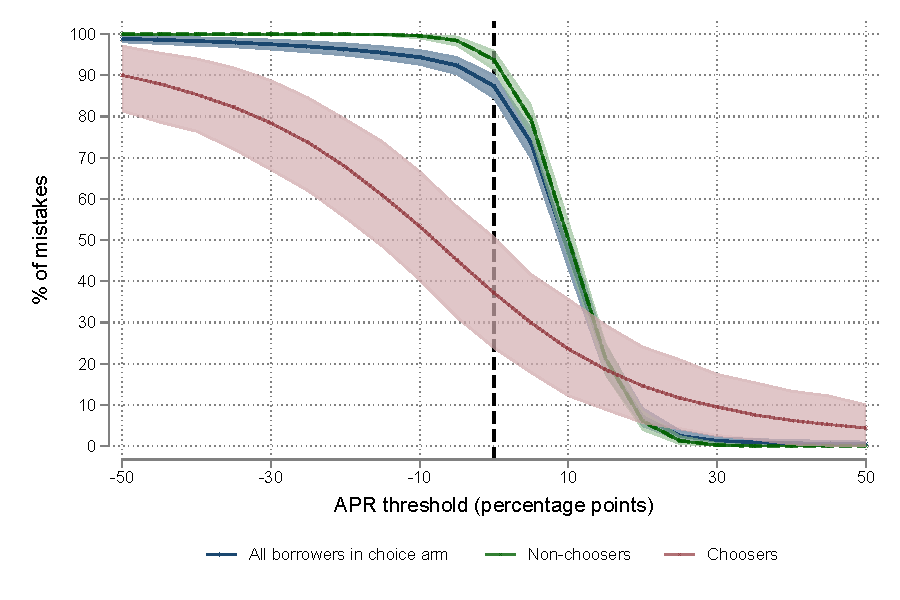
\includegraphics[width=0.6\textwidth]{Figuras/line_cw_apr_tot_tut.pdf}

 \end{center}       
 \caption{``Mistakes'' in the choice arm. This figure presents conditional average TUT and TOT effects for the APR outcome from Figure \ref{heterogeneous_effects} in an alternative manner, to consider the fraction of borrowers in the choice arm who made ``mistakes'' in their decision to accept or refuse the commitment contract. A ``mistake'' for a non-chooser is defined as a positive conditional TUT effect that significantly exceeds a specified threshold APR value.
%  The green curve equals $[1 - F_{\text{TUT}}(\delta)]\times 100\%$, where $F_{\text{TUT}}$ is the CDF corresponding to density of conditional TUT effects from Figure \ref{heterogeneous_effects}, computed using the instrumental forest approach from \cite{atheygrf}. Evaluated at any positive value on the horizontal axis, it gives the fraction of non-choosers in the choice arm who made a ``mistake'' by not choosing commitment. The green shaded region gives associated 95\% pointwise confidence bands. 
% Analogously, a ``mistake'' for a chooser is defined as a negative conditional TOT effect that exceeds a specified threshold APR value. The red curve equals $F_{\text{TOT}}(-\delta)$ where $F_{\text{TOT}}$ is the CDF corresponding to the density of conditional TOT effects from Figure \ref{heterogeneous_effects}. 
% The red shaded region gives associated 95\% pointwise confidence bands.
% For both the red and green curves, we define the APR threshold so that larger mistakes are to the \emph{right} of smaller mistakes.
% This allows us to construct the overall fraction of mistakes in the choice arm, the blue curve, as a weighted average of the green and red curves.
% The weights equal the share of choosers and non-choosers in the choice arm.
}
    \label{choose_wrong}
\end{figure}


The results in Figure \ref{choose_wrong} suggest that a large fraction of non-choosers made mistakes by not choosing commitment.
Even at an APR threshold as large as 10\%, we estimate that more than half of them should have chosen commitment in order to lower financial costs.
In contrast, relatively few choosers appear to have made mistakes by choosing commitment.
This now allows us to make a stronger statement in favor of paternalism in our context; not only does forced commitment generate large benefits on average, but it also benefits the vast majority of borrowers \emph{who would be coerced} under a policy of forced commitment.



\subsection{Can we target paternalism?}

Is it possible to target paternalism only towards those who would benefit from it?  A financial firm engageing in this type of targeting under real-world circumstances would be unable to use the subjective and unverifiable questions from the survey, and would not use the commitment choice since it will be unattractive for a company to ask consumer preferences and then force a product on those who had refused it. This leaves us with only a few objective covariates that could be used to target: age, gender, high school education or above, desired loan size, and whether that individual has ever pawned before. 
We call these the ``narrow'' covariate set, to contrast with the full set of survey variables, which we call the ``wide'' covariate set.  We take the estimated conditional average treatment effects (CATEs) $\widehat{\text{ATE}}(X_i)$ using the wide covariates as our ground truth, and now ask how well we can predict this benefit using the narrow covariate set.  Figure \ref{wide_narrow_forests} shows the relationship between these two different  CATEs.  We generate substantially less heterogeneity when using the narrow covariate set, although we still reject the null hypothesis of no treatment effect heterogeneity with the test from \cite{chernozhukov2018generic}.   To investigate targeting, we can assign a dummy variable equal to one for the 90\% of borrowers who have a positive CATE using the wide covariate set, and then implement both a logistic regression and a random forest classification model using only the narrow covariate set to predict positive benefits at the individual level.  


\begin{table}
\caption{Type I \& II errors using targeting narrow rules}
\label{hit_miss_rule}
\begin{center}

\scriptsize{% Table generated by Excel2LaTeX from sheet 'hit_miss_rule'
\begin{tabular}{lccc}
\toprule
\multicolumn{1}{c}{Rule} & \% incorrectly assigned to control  & \% incorrectly assigned to treatment & Overall Error Rate \\
\midrule
\midrule
All to control & 89.7  & 0     & 89.7 \\
All to forcing & 0     & 10.3  & 10.3 \\
Optimal & 0     & 0     & 0 \\
Narrow rule (RF) & 4.42  & 5.28  & 9.7 \\
Narrow rule (Logit) & 7.13  & 8.03  & 15.16 \\
Allow choice & 93.61 & 38.01 & 87.32 \\
\bottomrule
\bottomrule
\end{tabular}%
}

\end{center}
\legend{This table reports error rates for six different rules for allocating individuals to commitment. Row 1 assigns all borrowers to control, Row 2 all to the Forcing arm. Row 3 uses `optimal targeting according to the CATE from the wide covariate set. Row 4 uses a random forest classification, and Row 5 a logit model, both with only the narrow covariate set.  Row 6 uses the choices made by borrowers to assign to commitment.}
\end{table} 

We compare the in-sample performance of targeting rules against a policy of universal forced commitment. Table \ref{hit_miss_rule} shows error rates for six possible assignment rules: assigning all borrowers to control, all to treatment (Forcing), the optimal (infeasible) assignment, narrow RF targeting, Logit targeting, and the actual choice made by borrowers.  All models taking the wide RF as the ground truth. While the narrow RF correctly assigns roughly half of those who do not benefit from commitment to control, it also incorrectly allocates 4.38\% of the sample that would have gained from treatment to control. As such, it only improves the overall correct targeting rate by about half of a percentage point relative to universal Forcing. The Logit assignment rule is less successful at predicting benefits and harms, with a higher share of borrowers incorrectly assigned to both treatment and control, meaning that the overall correct targeting rate for the Logit is 5 pp lower than universal Forcing.  Self-targeting through choice proves to be little better than assigning everyone to the control condition, given the low take-up rate and the presence of both Type I and Type II errors in the choice arm.  The takeaway is that given low take-up, the large fraction of the sample benefiting from commitment, and the weak predictive power of the narrow covariates, in this case universal paternalism assigning all borrowers to the commitment contract appears to be an attractive targeting method.

    
\section{Conclusion} \label{conclusion}

This paper makes several contributions. First, it analyzes the large but understudied industry of pawn loans, and shows that a simple change to contract terms results in substantial financial savings for pawn borrowers: forced commitment lowers the APR from 57\% to 46\%, and reduces the fraction of borrowers who default by 6.6 pp, or 15\%. That this new contract generated large benefits for borrowers and yet was not offered, and that a contract that generated default was the industry standard instead, is related to the idea of ``veiled paternalism'' \cite{Laibson2018}, put on its head. In ``veiled paternalism'' principals embed forms of commitment into their products but mask this fact from consumers who may need but do not desire commitment, in pawn lending, over-collateralization means that lenders stand to make more money from defaulting borrowers, generating incentives for ``veiled \textit{non}-paternalism,'' embedding features that lead to high borrower costs in non-obvious ways.

%Potentially due to the nature of the borrower pool, 
%In our context voluntary commitment choice does improve borrower outcomes, but forcing commitment did induce significant cost savings for the overall group of clients.  


Second, our novel  ``controlled choice'' design allows us to go beyond ATE results and draw an important set of conclusions about the relationship between take-up and heterogeneous treatment effects. In particular, we simultaneously point-identify the impact of commitment on those who would naturally choose it \emph{and} those who only experience commitment when forced. Estimating this later quantity is critical in thinking about paternalism. We find substantial benefits of treatment for non-choosers and no evidence of selection on gains by borrowers who choose commitment. Given that the rate of voluntary commitment in our sample is only 11\%, in order to achieve widespread benefits in this context compulsory commitment appears to be necessary. 
%Clients appear to prefer the forced commitment after they have experienced it, in that assignment to this arm increases the fraction of individuals who return to pawn again.

Why do borrowers leave such substantial returns on the table? Our results suggest that over-optimism is the characteristic most strongly associated with benefiting from the commitment despite not having chosen it. Our borrower pool overestimates their probability of repayment by more than 50\%, and our positive TUT estimate is largely confined to borrowers who incorrectly believe that they have little chance of defaulting.  %More standard explanations such as discounting, learning, or time inconsistency find little support in our data. 

Using machine learning methods, we find the benefits of commitment close to universal. The benefits of targeting commitment based on characteristics that lenders can observe and participants would truthfully reveal are extremely limited, suggesting that universal commitment is an attractive policy in our empirical setting. 

%but the determinants that might allow us to target it more finely are primarily behavioral and hence not easily predicted in a fast incentive-compatible manner by lenders, making universal assignment to commitment attractive. Of course, in other applications this would have to be decided on a case-by-case basis.  %Even a sophisticated machine learning-based exercise is only able to decrease the fraction of borrowers mis-targeted less than half percentage points relative to simply assigning everyone to commitment (from 9.78\% to 9.59\%).  and a logit-based targeting rule actually does slightly worse than universal commitment.  

Where lenders have no incentive to engage in veiled paternalism and customers display inefficiently low demand for it, financial policy regulation may prove an attractive option.  Pawnshops, along with other over-collateralized credit products such as payday lending, exist in an environment where the lender may desire customers to lose their collateral on the loan, hurting especially low-income populations who are its main users. With a now well-established toolkit of regular small payments and incentives delivering small default rates in microfinance, regulators may fruitfully investigate the possibility of requiring pawnbrokers to embed features of commitment and regularity into their repayment structures in more consistent ways.\footnote{If employed at scale in a competitive lending sector this would redistribute welfare from those who would have repaid (whose interest rates must now rise to cover lower returns from collateral seizure) towards those who would only repay in the presence of commitment. In a setting of lender market power however, redistribution from lenders to borrowers could occur.}
An important question for future research will be the extent to which borrowers are able to learn about the benefits of commitment over time, making it so that temporary, lighter-touch policies could achieve lasting benefits for borrowers.  Pawning with commitment may provide an important mechanism to preserve flexible credit access while allowing more poor borrowers to retain their assets.

%%%%%%%%%%%%%%%%%%%%%%%%%%%%%%%%%%%%%%%%%%%%%%%%%%%%%%%%%%%%%
%BIBLIOGRAPHY


\bibliographystyle{ecta-fullname} % Style BST file
\bibliography{References}  % Bibliography file (usually '*.bib')

%%%%%%%%%%%%%%%%%%%%%%%%%%%%%%%%%%%%%%%%%%
% Proofs below
%%%%%%%%%%%%%%%%%%%%%%%%%%%%%%%%%%%%%%%%%%

\section{Proofs}
\label{sec:proofs}

This section gives a formal derivation of the identification results presented in Equations \eqref{eq:TOT}--\eqref{eq:ASL} of \autoref{sec:randchoice}.
To simplify the presentation, we omit $i$ subscripts throughout.
%and adopt the shorthand  $Z_0 \equiv \mathbbm{1}(Z=0)$, $Z_1 \equiv \mathbbm{1}(Z=1)$, and $Z_2 \equiv\mathbbm{1}(Z=2)$.
%The following assumption collects our exclusion restriction and the key features of the constrained choice design.

\begin{assumption}[Randomized Choice Design and Exclusion Restriction]\mbox{}
\label{assump:randchoice}
   \begin{enumerate}[(i)]
   \item $Z$ is independent of $(Y_{0}, Y_{1}, C)$
   \item $D = \mathbbm{1}(Z \neq 2)Z + \mathbbm{1}(Z = 2)C$
   \item $Y = \mathbbm{1}(Z = 0) Y_{0} + \mathbbm{1}(Z = 1) Y_{1} + \mathbbm{1}(Z = 2) [ (1 - C) Y_{0} + C Y_{1}]$
   \end{enumerate}
\end{assumption}

\begin{lem}
Under Assumption \ref{assump:randchoice},
\label{lem_randchoice}
   \begin{enumerate}[(i)]
       \item $\mathbbm{E}(D|Z=2) = \mathbb{P}(C=1)$
       \item $\mathbbm{E}(Y|Z=0) = \mathbbm{E}(Y_0)$
       \item $\mathbbm{E}(Y|Z=1) = \mathbbm{E}(Y_1)$
       \item $\mathbbm{E}(Y|D=0,Z=2) = \mathbbm{E}(Y_0|C=0)$
       \item $\mathbbm{E}(Y|D=1,Z=2) = \mathbbm{E}(Y_1|C=1)$.
   \end{enumerate} 
\end{lem}

\begin{proof}
Part (i) follows because $Z=2$ implies $D=C$ and $Z$ is independent of $C$.  
Parts (ii) and (iii) follow similarly: given $Z=0$ we have $Y = Y_0$, given $Z=1$ we have $Y = Y_1$, and $Z$ is independent of $(Y_0,Y_1)$.
For parts (iv) and (v), first note that Assumption \ref{assump:randchoice} (iii) implies that $Z$ is conditionally independent of $(Y_0,Y_1)$ given $C$.
Now, $Z=2$ implies that $D=0$ if and only if $C=0$. Hence, $\mathbbm{E}(Y|D=0, Z=2) = \mathbbm{E}(Y_0|C=0)$ establishing part (iv).
For part (v) $Z=2$ implies that $D=1$ if and only if $C=1$ from which it follows that $\mathbbm{E}(Y|D=1, Z=2) = \mathbbm{E}(Y_1|C=1)$.
\end{proof}

\begin{prop} 
Under Assumption \ref{assump:randchoice},
    \begin{enumerate}[(i)]
        \item $\text{TOT} \equiv \mathbbm{E}(Y_1 - Y_0|C=1)  = \displaystyle \frac{\mathbbm{E}(Y|Z=2) - \mathbbm{E}(Y|Z=0)}{\mathbbm{E}(D|Z=2)}$
        \item $\text{TUT} \equiv \mathbbm{E}(Y_1 - Y_0|C=0) = \displaystyle \frac{\mathbbm{E}(Y|Z=1) - \mathbbm{E}(Y|Z=2)}{1 - \mathbbm{E}(D|Z=2)}$
        \item $\text{ASB} \equiv \mathbbm{E}(Y_0|C=1) - \mathbbm{E}(Y_0|C=0) = \displaystyle \frac{\mathbbm{E}(Y|Z=0) - \mathbbm{E}(Y|Z=2,D=0)}{\mathbbm{E}(D|Z=2)}$
        \item $\text{ASL} \equiv \mathbbm{E}(Y_1|C=1) - \mathbbm{E}(Y_1|C=0) = \displaystyle \frac{\mathbbm{E}(Y|Z=2,D=1) - \mathbbm{E}(Y|Z=1)}{1 - \mathbbm{E}(D|Z=2)}$.
    \end{enumerate}
\end{prop}

\begin{proof}
Parts (i) and (iii) we require an expression for $\mathbbm{E}(Y_0|C=1)$ in terms of $(Y, D, Z)$.
By Lemma \ref{lem_randchoice}(ii) and iterated expectations 
\[
\mathbbm{E}(Y|Z=0) = \mathbbm{E}(Y_0) = \mathbbm{E}(Y_0|C=0) \mathbbm{P}(C=0) + \mathbbm{E}(Y_0|C=1) \mathbbm{P}(C=1).
\]
Re-arranging and substituting Lemma \ref{lem_randchoice}(i) and (iv),
\begin{align}
\mathbbm{E}(Y_0|C=1)  
%&= \frac{\mathbbm{E}(Y|Z=0) - \mathbbm{E}(Y_0|C=0) \mathbbm{P}(C=0)}{\mathbbm{P}(C=1)}\nonumber\\ 
&=  \frac{\mathbbm{E}(Y|Z=0) - \mathbbm{E}(Y|Z=2,D=0) \mathbbm{E}(1 - D|Z=2)}{\mathbbm{E}(D|Z=2)}.
\label{eq:Y0C1}
\end{align}
Part (i) follows by combining \eqref{eq:Y0C1} with Lemma \ref{lem_randchoice}(v) and simplifying; part (iii) follows by combining \eqref{eq:Y0C1} with Lemma \ref{lem_randchoice}(iv) and simplifying.
Similarly, for parts (ii) and (iv) we require an expression for $\mathbbm{E}(Y_1|C=0)$ in terms of observables.
By Lemma \ref{lem_randchoice}(iii) and iterated expectations,
\[
\mathbbm{E}(Y|Z=1) = \mathbbm{E}(Y_1) = \mathbbm{E}(Y_1|C=0)\mathbbm{P}(C=0) + \mathbbm{E}(Y_1|C=1) \mathbbm{P}(C=1).
\]
Re-arranging and substituting Lemma \ref{lem_randchoice}(i) and (v),
\begin{align}
\mathbbm{E}(Y_1|C=0) 
%&= \frac{\mathbbm{E}(Y|Z=1) - \mathbbm{E}(Y_1|C=1)\mathbbm{P}(C=1)}{\mathbb{P}(D=0)} \nonumber\\
&=\frac{\mathbbm{E}(Y|Z=1) - \mathbbm{E}(Y|Z=2,D=1)\mathbbm{E}(D|Z=2)}{\mathbb{E}(1-D|Z=2)}.
\label{eq:Y1C0}
\end{align}
Part (ii) follows by combining \eqref{eq:Y1C0} with Lemma \ref{lem_randchoice}(iv) and simplifying; part (iv) follows by combining \eqref{eq:Y1C0} with Lemma \ref{lem_randchoice}(v) and simplifying.
\end{proof}

\newpage



\pagenumbering{arabic}
\renewcommand\thefigure{OA-\arabic{figure}}
\renewcommand\thetable{OA-\arabic{table}}
\renewcommand*{\thepage}{OA - \arabic{page}}
\renewcommand\thesection{Appendix \Alph{section}.}
\renewcommand\thesubsection{\Alph{section}.\arabic{subsection}}




\begin{frontmatter}

\title{The controlled choice design and private paternalism in pawnshop borrowing - ONLINE APPENDIX}
\runtitle{The controlled choice design and private paternalism}

\begin{aug}
% use \particle for den|der|de|van|von (only lc!)
% [id=?,addressref=?,corref]{\fnms{}~\snm{}\ead[label=e?]{}\thanksref{}}
%
%% e-mail is mandatory for each author
%
%%% initials in fnms (if any) with spaces
%
\author[id=au1,addressref={add1}]{\fnms{Craig}~\snm{McIntosh}\ead[label=ee1]{ctmcintosh@ucsd.edu}}
\author[id=au2,addressref={add2}]{\fnms{Isaac}~\snm{Meza}\ead[label=ee2]{isaacmezalopez@g.harvard.edu}}
\author[id=au3,addressref={add3}]{\fnms{Joyce}~\snm{Sadka}\ead[label=ee3]{jsadka@itam.mx}}
\author[id=au4,addressref={add4}]{\fnms{Enrique}~\snm{Seira}\ead[label=ee4]{enrique.seira@gmail.com}}
\author[id=au5,addressref={add5}]{\fnms{Francis J.}~\snm{DiTraglia}\ead[label=ee5]{francis.ditraglia@economics.ox.ac.uk}}

% Addresses
\address[id=add1]{%
\orgdiv{Department of Economics}
\orgname{University of California San Diego}}

\address[id=add2]{%
\orgdiv{Department of Economics}
\orgname{Harvard University}}

\address[id=add3]{%
\orgdiv{Department of Economics}
\orgname{Instituto Tecnologico Autonomo de Mexico}}

\address[id=add4]{%
\orgdiv{Department of Economics}
\orgname{Michigan State University}}

\address[id=add5]{%
\orgdiv{Department of Economics}
\orgname{University of Oxford}}
\end{aug}


\end{frontmatter}

\begin{appendix}
    

\section{Treatment Explanation Materials and Pictures}

\subsection{Materials}

\begin{figure}[!htb]
     \caption{Contract Terms Summary}
    \label{PaperSlip}
    \begin{center}
        \includegraphics[width=0.7\textwidth]{Figuras/TicketLenderP.png}
    \end{center}
    \legend{We show a sample receipt that was given to clients that got assigned to the fee-forcing contract (the font and format were changed to protect Lender's P identity). We want to highlight the salience of some items. First the title clearly indicated which contract the client has (arrow 1). Second, in the case of the fee contract it clearly indicates that there is a fee for paying late equivalent to 2\% of the value of the monthly payment (arrow 2). Third, there is a calendar for payments clearly specifying the dates and amounts to pay each month.}
\end{figure}

\begin{figure}[!htb]
     \caption{Explanatory Material}
    \label{ExplanatoryMaterial}
    \begin{center}
    \begin{subfigure}{\textwidth}
        \centering
        \includegraphics[width=0.7\textwidth]{Figuras/micas.pdf}
    \end{subfigure}
    \end{center}
    \legend{ This is a (translated) sample information slide shown to clients. The real ones were twice the size of this figure and were laminated. Different ones were shown for each treatment arm.}
\end{figure}



\subsection{Pictures}

\begin{figure}[!htb]
     \caption{Some Pawnshops}
    \label{PawnshopPicture}
    \begin{center}
    \begin{subfigure}{0.405\textwidth}
    \caption{Appraiser/tellers inside a pawnshop}
        \centering
        \includegraphics[width=\textwidth]{Figuras/empenio9_.png}
    \end{subfigure}
        \begin{subfigure}{0.45\textwidth}
    \caption{Pawnshop}
        \centering
        \includegraphics[width=\textwidth]{Figuras/empenio11_.png}
    \end{subfigure}
    
        \vspace{3ex}

    \begin{subfigure}{0.45\textwidth}
    \caption{Pawnshop}
        \centering
        \includegraphics[width=\textwidth]{Figuras/empenio2_.png}
    \end{subfigure}
    \begin{subfigure}{0.415\textwidth}
    \caption{Lost pawns which are for sale}
        \centering
        \includegraphics[width=\textwidth]{Figuras/empenio3_.png}
    \end{subfigure}
    \end{center}
   \legend{ This figure  shows pictures of pawnshops in Mexico city. They do not necessarily coincide with Lender P for confidentiality. }
\end{figure}




\begin{figure}[!htb]
     \caption{Gold buyers next to pawnshops}
    \label{GoldBuyers}
    \begin{center}
    \begin{subfigure}{.49\textwidth}
    \caption{Gold buyer next to pawnshop 1}
        \centering
        \includegraphics[width=\textwidth]{Figuras/empenio7_.png}
    \end{subfigure}
    \begin{subfigure}{.49\textwidth}
    \caption{Gold buyer next to pawnshop 1}
        \centering
        \includegraphics[width=\textwidth]{Figuras/empenio8_.png}
    \end{subfigure}
       \vspace{3ex}
       
    \end{center}
    \legend{  This figure shows pictures of gold buyers next to pawnshops in Mexico city. They do not necessarily coincide with Lender P for confidentiality. }
\end{figure}


\subsection{Descriptives consistent with overconfidence}

\vspace{.2in}
\begin{figure}[!htb]
    \caption{Behavior of borrowers who lost their pawn}
    \label{proxy_naive}
    \begin{center}
    \begin{subfigure}{0.40\textwidth}
        \caption{Elapsed days to first payment}
        \centering
        \includegraphics[width=\textwidth]{Figuras/hist_firstdays_default.pdf}
    \end{subfigure}
    \begin{subfigure}{0.40\textwidth}
        \caption{Elapsed days to last payment}
        \centering
        \includegraphics[width=\textwidth]{Figuras/hist_days_default.pdf}
    \end{subfigure}
        \begin{subfigure}{0.40\textwidth}
        \caption{Payments as \% of loan}
        \centering
        \includegraphics[width=\textwidth]{Figuras/hist_percpay_default.pdf}
    \end{subfigure}
    \begin{subfigure}{0.40\textwidth}
        \caption{Number of payments}
        \centering
        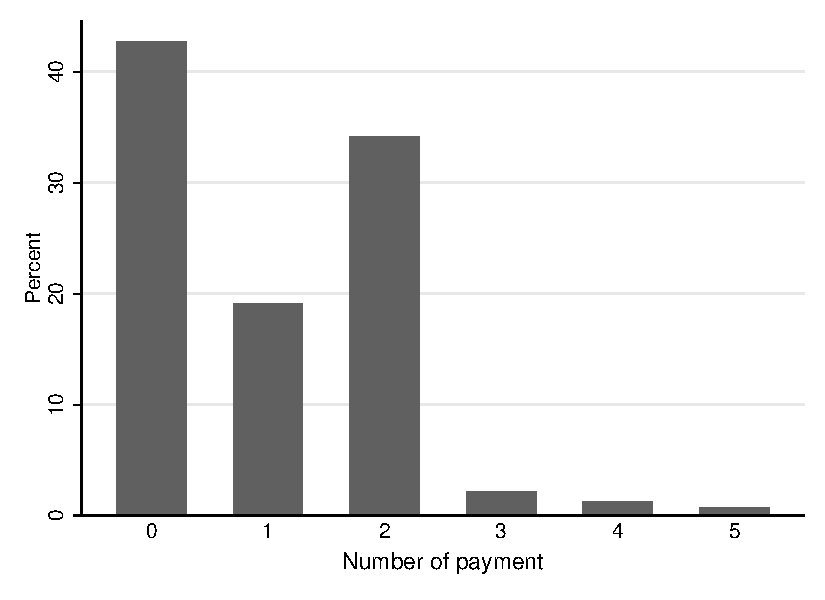
\includegraphics[width=\textwidth]{Figuras/hist_numpay_default.pdf}
    \end{subfigure}
    \end{center}
       \legend{ This figure provides more details on the behavior of clients who were assigned to the control group and did not recover their pawn. Panel (a) shows a histogram of days elapsed from the pawn to the first payment, while panel (b) displays a histogram of days elapsed until the last payment. Some borrowers make payments after day 105, the end of the grace period: if they pay all interest owed, they can ``restart'' the loan. This amounts to starting a new loan with the same conditions and same pawn. Panel (c) shows a histogram of the fraction of the loan paid, while panel (d) presents a barplot of the number of times that borrowers went to the branch to make payments.}
      %\textit{Do file: }  \texttt{hist\_den\_default.do}
\end{figure}

    
\section{Internal Validity}

\subsection{Survey}   \label{app:survey_data}

We now present analysis of the extent to which the survey-responding sample is representative and balanced.
Table \ref{SS_cond_survet} presents information about survey non-response.
Panel A is a balance table that compares loan amount and day of the week across treatment arms for the subset of borrowers who responded to at least one survey question.
The p-values in the fourth column are for the F-test of no difference of means across treatment arms. 
Panel B presents response-rates by question for each arm of the experiment, along with p-values for the F-test of no difference in question-specific response rates across treatment arms. 
This panel uses data from participants who answered at least one survey question and went on to pawn on the same day as their survey response.
From the table, we see that loan amount and weekday are balanced across treatment arms among survey respondents and that response rates are likewise stable across treatment arms.
Table \ref{TUT_cond_survet} shows how the estimated TUT effect changes if we restrict our estimation sample based on survey response.
The first row of the table presents TUT results for the financial cost outcome, while the second presents corresponding results for the APR outcome.
In each row, column (1) presents the full-sample TUT estimate and standard error while the remaining columns restrict the sample to borrowers who answered a particular survey question or set of questions.
For example, column (4) presents results for borrowers who answered the two questions needed to compute our measure of ``present bias'' discussed in the next paragraph, while column (9) present results restricted to participants who disclosed their sex. 
As seen from the table, our TUT estimates are quite stable across sub-samples defined by survey response.
In each case they are positive and of the same magnitude as the corresponding full-sample estimate, although statistical significance varies depending on the size of the corresponding sub-sample. 
For these reasons, we are comfortable relying on data for survey respondents in the empirical exercises that follow.
In exercises that rely on a single survey question, we use data for every borrower who answered that question.
In the random forest exercises described below, we use data for every borrower who answered at least one survey question.



\begin{table}[!htb]
\caption{Baseline survey questions (translated to English)}
\label{baseline_survey}
\begin{center}
\scriptsize{% Table generated by Excel2LaTeX from sheet 'transcribed'
\begin{tabular}{cl}
\toprule
      & \textbf{Baseline Survey} \\
\midrule
\midrule
1     & \textbf{Your pawn was:} \\
      & (a) Inherite, (b) a gift, (c) bought by me, (d) lend to me, (e) other \_\_\_\_\_\_\_\_\_\_\_\_ \\
2     & \textbf{Mark with an "X" in the line below how likely is that you recover your pawn. } \\
      & \textbf{Where 0 is impossible and 100 is completely certain} \\
3     & \textbf{How much would you sell the item you want to pawn for?       \_\_\_\_\_\_\_\_\_\_\_\_\_\_ pesos} \\
4     & \textbf{Gender      } \\
5     & \textbf{Age} \\
6     & \textbf{Civil Status } \\
      & (a) married, (b) single, (c) divorced, (d) widowed \\
7     & \textbf{Work status} \\
      & (a) employed, (b) own business, (c) houseshores, (d) don't work, (e) retired, (f) study \\
8     & \textbf{Education} \\
      & (a) no formal education, (b) primary, (c) middle school, (d) highschool, (e) more than highschool \\
9     & \textbf{In the last month, did a friend or family member asked you for money?} \\
      & (a) yes  (b) no \\
10    & \textbf{What would you like to have: 100 pesos tomorrow or 150 pesos in one month?} \\
11    & \textbf{How often do you feel stressed by your economic situation?} \\
      & (a) always, (b) very often, (c) sometimes, (d) never \\
12    & \textbf{What is the main reason you want to pawn?} \\
      & (a) Need the money because somebody in my family lost his/her job \\
      & (b) Need the money to pay for a sickness in the family \\
      & (c) Need the money for an urgent expense \\
      & (d) Need the money for some non urgent expense. \\
13    & \textbf{How stressed do you feel from the situation that led to to pawn?} \\
      & (a) very stressed, (b) somwhat stressed, (c) a little stressed, (d) not stressed  \\
14    & \textbf{In 3 months, I expect to have a  \_\_\_\_\_\_\_\_\_\_\_\_\_\_\_\_ situation} \\
      & (a) better, (b) similar,  (c) worse \\
15    & \textbf{Have you panwned before?} \\
      & (a) yes  (b) no \\
16    & \textbf{How many times have you pawned on a Lender P branch?} \\
      & (a) NO\_\_\_    (b)  1-2 times \_\_\_    (c) 3-5 times\_\_\_\_   (d) More than 5\_\_\_\_ \\
17    & \textbf{If you are saving money and a family member wants to use it for something } \\
      & (a) I would only give him the money for an urgent expenze \\
      & (b) I would give him the money even if it was not an urgent expense \\
      & (c) I would not give him/her the money regardless \\
      & (d) No one would ask me for my money \\
18    & \textbf{Do you make an expenses budget for the month ahead of time?} \\
      & (a) always, (b) very often, (c) sometimes, (d) never \\
19    & \textbf{Do you have other items you could pawn?} \\
      & (a) yes  (b) no \\
20    & \textbf{Do you have savings?} \\
      & (a) yes  (b) no \\
21    & \textbf{Do you participate in a ROSCA?} \\
      & (a) yes  (b) no \\
22    & \textbf{Is it common that family or friends ask for money?} \\
      & (a) yes  (b) no \\
23    & \textbf{How much did you spend to come to the branch today?    \$\_\_\_\_\_\_\_\_\_\_\_\_\_\_ pesos} \\
24    & \textbf{How much time does it usually take to come to this branch?    \_\_\_\_\_\_\_\_\_\_\_} \\
25    & \textbf{How much does your family spend in a normal week?   \$\_\_\_\_\_\_\_\_\_\_\_\_\_\_ pesos} \\
26    & \textbf{How much do you manage to save in a normal week?   \$\_\_\_\_\_\_\_\_\_\_\_\_\_\_ pesos} \\
27    & \textbf{Does it happen to you that you spend more than you wanted because you fall into temptation?} \\
      & (a) never, (b) almost never, (c) sometimes, (d) very often \\
28    & \textbf{In the last 6 months, has it happened that at some point you lacked money to pay} \\
      & (a) rent?    (b) food    (c)food   (d) medicine  (e) electricity   (f) heating   (g) telephone    (i) water \\
29    & \textbf{What would you like to have: 100 pesos in 3 months or 150 pesos in four months?} \\
30    & \textbf{Would you like to receive (free) reminders for upcomming payments?} \\
      & (a) yes  (b) no \\
\bottomrule
\end{tabular}%
}
\end{center}
\legend{ Translation of the baseline questionnaire.}
\end{table}


\begin{figure}[!htb]
     \caption{Box-plot across arms}
    \label{boxplot_attrition}
    \begin{center}
    \begin{subfigure}{0.45\textwidth}
    \caption{Number of pawns}
        \centering
        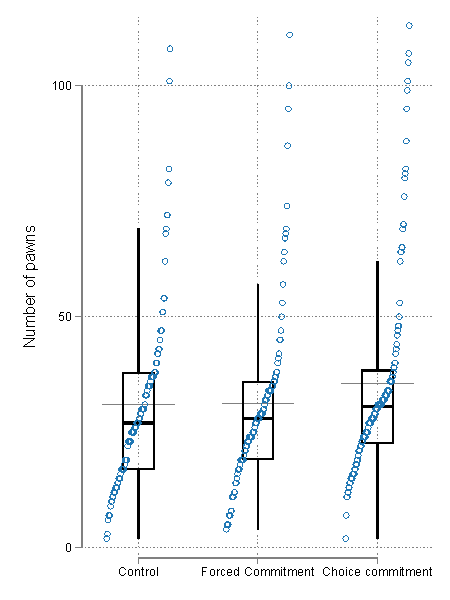
\includegraphics[width=\textwidth]{Figuras/box_plot_num_pawns.pdf}
    \end{subfigure}
        \begin{subfigure}{0.45\textwidth}
    \caption{Number of borrowers}
        \centering
        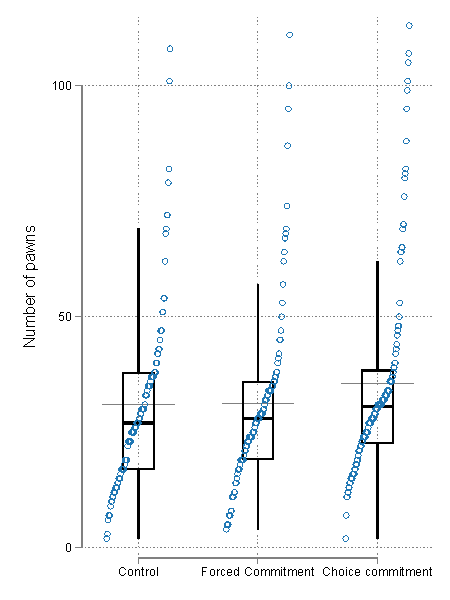
\includegraphics[width=\textwidth]{Figuras/box_plot_num_pawns.pdf}
    \end{subfigure}
    \end{center}
    \legend{ This figure presents box-plot for the number of pawns and borrowers per branch-day across different arms. The solid black line represent the median, while the gray line represent the mean. The dots on top of the box-plot represent an implicit CDF. }
\end{figure}




\begin{table}[!htb]
\caption{Balance conditional on survey response and question-by-question response rates by treatment arm}
\label{SS_cond_survet}
\begin{center}
\scriptsize{% Table generated by Excel2LaTeX from sheet 'SS_cond_survey'
\begin{tabular}{lcccc}
\toprule
      &       & \multicolumn{3}{c}{Commitment arms} \\
\cmidrule{3-5}      & \multicolumn{1}{p{4.5em}}{Control} & \multicolumn{1}{p{4.93em}}{Forced} & \multicolumn{1}{p{3.43em}}{Choice} & \multicolumn{1}{p{3.43em}}{p-value} \\
\midrule
      & \multicolumn{4}{c}{Panel A : Administrative Data (conditional on survey)} \\
\midrule
\midrule
Loan amount  & 2199  & 2196  & 2216  & 0.98 \\
      & (86)  & (106) & (81)  &  \\
Weekday & 0.88  & 0.89  & 0.85  & 0.8 \\
      & (0.045) & (0.038) & (0.045) &  \\
\midrule
Obs   & 1386  & 1469  & 1982  &  \\
\midrule
      & \multicolumn{4}{c}{Panel B : Survey Data - response rate} \\
\midrule
\midrule
Subjective value & 0.73  & 0.69  & 0.71  & 0.39 \\
      & (0.022) & (0.024) & (0.024) &  \\
Trouble paying bills & 0.49  & 0.48  & 0.44  & 0.29 \\
      & (0.023) & (0.022) & (0.022) &  \\
Present bias & 0.43  & 0.44  & 0.39  & 0.17 \\
      & (0.02) & (0.02) & (0.02) &  \\
Makes budget & 0.55  & 0.56  & 0.53  & 0.56 \\
      & (0.023) & (0.023) & (0.019) &  \\
Subj. pr. of recovery & 0.74  & 0.72  & 0.74  & 0.71 \\
      & (0.024) & (0.025) & (0.025) &  \\
Pawn before & 0.55  & 0.57  & 0.53  & 0.57 \\
      & (0.023) & (0.024) & (0.02) &  \\
Age   & 0.54  & 0.55  & 0.52  & 0.59 \\
      & (0.023) & (0.023) & (0.018) &  \\
Woman & 0.58  & 0.59  & 0.58  & 0.93 \\
      & (0.025) & (0.024) & (0.02) &  \\
+ High-school & 0.54  & 0.55  & 0.51  & 0.39 \\
      & (0.025) & (0.025) & (0.019) &  \\
\midrule
Obs   & 1386  & 1469  & 1982  &  \\
\bottomrule
\bottomrule
\end{tabular}%
}
\end{center}
\legend{ Panel A of this table presents the same information as Panel A of Table \ref{SS}, but restricts attention to the subsample of borrowers who answered at least one question in our baseline survey. Conditional on survey response, loan amount and weekday are balanced across treatment arms. Panel B presents response rates to each individual survey question across treatment arms, along with p-values for the F-test of no difference in response rates across survey arms. This panel uses data for borrowers who pawned on the same day as their survey response. }


%\textit{Do file: } \texttt{ss\_att.do}
\end{table}



\begin{landscape}
\begin{table}[!htb]
\caption{Survey Non-response: TUT estimates for respondents to each survey question.}
\label{TUT_cond_survet}
\begin{center}
\scriptsize{% Table generated by Excel2LaTeX from sheet 'tut_cond_survey'
\begin{tabular}{lcccccccccc}
\toprule
      & Full-sample & Subjective value & Trouble paying bills & Present bias & Makes budget & Subj. pr. of recovery & Pawn before & Age   & Woman & + High-school \\
\midrule
      & (1)   & (2)   & (3)   & (4)   & (5)   & (6)   & (7)   & (8)   & (9)   & (10) \\
\midrule
\midrule
Apr \% benefit & 10.3*** & 10.4*** & 11.3*** & 12.0*** & 10.4*** & 11.2*** & 10.5*** & 11.0*** & 11.5*** & 11.0*** \\
      & (2.44) & (2.36) & (2.59) & (2.64) & (2.68) & (2.29) & (2.67) & (2.89) & (2.91) & (2.84) \\
      &       &       &       &       &       &       &       &       &       &  \\
\midrule
      & (11)  & (12)  & (13)  & (14)  & (15)  & (16)  & (17)  & (18)  & (19)  & (20) \\
\midrule
\midrule
FC benefit TuT & 187.1*** & 185.6*** & 143.7** & 183.9** & 154.9** & 181.2*** & 141.4** & 160.7** & 138.0** & 129.0* \\
      & (50.7) & (58.0) & (67.6) & (81.9) & (69.8) & (60.7) & (68.5) & (74.5) & (69.1) & (72.5) \\
      &       &       &       &       &       &       &       &       &       &  \\
\midrule
Observations & 6304  & 4465  & 2948  & 2613  & 3433  & 4625  & 3468  & 3393  & 3677  & 3352 \\
\bottomrule
\bottomrule
\end{tabular}%
}
\end{center}
\legend{ Some borrowers did not respond to our survey; others only completed part of the survey.
This table computes the TUT effect for a number of sub-groups by survey response, and compares them against the overall TUT effect.
The top panel uses financial cost as the outcome variable, while the bottom panel uses APR.
Each group is defined by the borrowers who responded to a particular \emph{subset} of the survey questions. 
For example, column (4) computes TUT effects for the subgroup of borrowers who responded to the two questions needed to compute our measure of present bias, while column (8) computes the TUT for the subgroup of borrowers who provided their age.
The bottom row of the table counts the number of borrowers in each category.
TUT estimates are quite stable across sub-groups and generally similar to the full-sample estimates.
Because standard errors increase as sample size falls, some of the sub-group estimates are not statistically significant.}
%\textit{Do file: } \texttt{tut_cond_survey.do}
\end{table}
\end{landscape}



\section{Main treatment effects: Additional material}


\begin{landscape}
\subsection{Multiple loans}

\begin{table}[!htb]
\caption{Multiple-loans robustness check}
\label{multiple_loans}
\begin{center}
\scriptsize{% Table generated by Excel2LaTeX from sheet 'multiple_loans'
\begin{tabular}{lcccccccccccccc}
\toprule
      & \multicolumn{4}{c}{First visit (Baseline approach)} &       & \multicolumn{4}{c}{Multiple visits - multiple treatments} &       & \multicolumn{4}{c}{First treatment (ITT)} \\
\cmidrule{7-10}\cmidrule{12-15}      & FC    & APR   & Recovery & Default &       & FC    & APR   & Recovery & Default &       & FC    & APR   & Recovery & Default \\
\midrule
      & (1)   & (2)   & (3)   & (4)   &       & (5)   & (6)   & (7)   & (8)   &       & (9)   & (10)  & (11)  & (12) \\
\midrule
\midrule
Forced Commitment & -202.8*** & -0.11*** & 0.14*** & -0.065*** &       & -175.2*** & -0.078*** & 0.099*** & -0.032 &       & -159.1*** & -0.086*** & 0.11*** & -0.051*** \\
      & (48.1) & (0.019) & (0.025) & (0.023) &       & (42.8) & (0.017) & (0.021) & (0.020) &       & (38.6) & (0.015) & (0.021) & (0.019) \\
Choice Commitment & -39.6 & -0.0089 & 0.0094 & -0.024 &       & -34.4 & 0.0028 & 0.00054 & -0.0049 &       & -31.5 & -0.017 & 0.029 & -0.032* \\
      & (49.8) & (0.019) & (0.022) & (0.021) &       & (43.5) & (0.016) & (0.018) & (0.018) &       & (40.4) & (0.014) & (0.018) & (0.018) \\
      &       &       &       &       &       &       &       &       &       &       &       &       &       &  \\
\midrule
Observations & 6304  & 6304  & 6304  & 6304  &       & 8519  & 8519  & 8519  & 8519  &       & 8813  & 8813  & 8813  & 8813 \\
R-sq  & 0.013 & 0.031 & 0.019 & 0.013 &       & 0.016 & 0.032 & 0.018 & 0.010 &       & 0.016 & 0.031 & 0.020 & 0.015 \\
Control Mean & 941.3 & 0.57  & 0.43  & 0.44  &       & 905.7 & 0.54  & 0.46  & 0.42  &       & 904.7 & 0.55  & 0.44  & 0.44 \\
\bottomrule
\bottomrule
\end{tabular}%
}
\end{center}
 \legend{ An additional empirical issue generated by repeat pawning is the question of how to handle the treatment status of those who take multiple loans within the experiment.  43\% of borrowers take more than one loan within the study period, and 19\% are assigned multiple treatment statuses on their different loans.  The issue of sequential endogenous treatments has been extensively studied in the context of school lotteries, where the convention is to use the treatment status from the first exposure (ITT) \citep{cullen2006effect, abdulkadirouglu2011accountability}.\\
 This table provides robustness for our main results for different ways to handling the multiplicity of loans. Columns 1-4 repeat the main analysis of financial cost and APR using the baseline approach from our main results,i.e. it only considers the first visit, while allowing multiple loans for the same-day. Columns 5-8 considers all loans including dummies for the order of pawns for an individual, essentially making the identification within-order.  Columns 9-12 pursue the ITT strategy of always assigning the first treatment status to all subsequent pawns. The core treatment effects are robust to any of these ways of handling repeat pawning.  }
 
%\textit{Do file: } \texttt{multiple\_loans.do}
\end{table}


\end{landscape}


\begin{figure}[!htb]
    \caption{Determinants of choice}
    \label{determinants_choose}
    \begin{center}
    \begin{subfigure}{0.5\textwidth}
        \centering
        \includegraphics[width=\textwidth]{Figuras/determinants_choose_commitment.pdf}
    \end{subfigure}
    \end{center}
      \legend{  The above figure shows the determinants in a bivariate and multivariate OLS regression of choosing commitment. Choice commitment is a binary variable equal to one, whenever subjects choose the forced commitment contract in the choice arm. }
%\textit{Do file: } \texttt{determinants_choice.do}       
\end{figure}


\vspace{.2in}
\begin{figure}[!htb]
    \caption{Histogram of payments}
    \label{hist_payments}
    \begin{center}
    \begin{subfigure}{0.32\textwidth}
        \caption{Status-quo}
        \centering
        \includegraphics[width=\textwidth]{Figuras/hist_payments_sq.pdf}
    \end{subfigure}
    \begin{subfigure}{0.32\textwidth}
        \caption{Forced commitment}
        \centering
        \includegraphics[width=\textwidth]{Figuras/hist_payments_fc.pdf}
    \end{subfigure}
    \begin{subfigure}{0.32\textwidth}
        \caption{Choice commitment}
        \centering
        \includegraphics[width=\textwidth]{Figuras/hist_payments_cc.pdf}
    \end{subfigure}    
    \end{center}
     \legend{ This figure shows the schedule of payments for each treatment arm. In other words it records the time after the loan origination when the borrower makes a payment toward recovery of the pawn. We can see that for both the Forced commitment and Choice commitment arm, payments are bunching at the 30 and 60 days, while most payments are done around the due date of the loan (90 days).}
     
      %\footnotesize{ \textit{Do file: }  \texttt{hist\_payments.do}}
\end{figure}




\subsection{Censoring} \label{App_censoring}


Some loans in our sample are ``censored'' in that they continue beyond our observation period.
For these loans, we do not know whether the borrower ultimately defaulted or recovered her pawn.
In this appendix, we show that our main results are robust to different ways of addressing censoring.

Our main results, presented above, make no assumption on the default/recovery status of this loans. However, we compute the Financial Cost \& APR considering all the payments done so far. We now consider some alternative approaches. \\
  

One way of considering the effect that this issue could have on our results is to make extreme assumptions about the outcome of these loans in the treatment and control so as to bound the possible influence of censoring.  In Table \ref{bounding_censoring} we compare the Forced and Control arms, making the bracketing assumptions about repayment on censored loans.  Panel A assumes all censored loans are repaid, and Panel D that all default. Because forced commitment causes borrowers to make payments earlier than they otherwise would have, In Panel A we make a conservative assumption. To see why, suppose for the sake of argument that commitment affects payment timing, but does not not default.
In other words, suppose that treatment makes censoring \emph{less likely} but has no effect on uncensored outcomes. 
If we were to treat all outstanding loans as defaults--the opposite of our convention--this would artificially inflate the rate of default among control loans relative to treatment loans.

Panel B provides the lower bound for the treatment effect by assuming censored control loans are always repaid and treatment loans never are, and Panel C the upper bound by making the reverse assumption.  Comfortingly, even with these extreme assumptions the significance on the main treatment effects never flips and treatment effects on financial cost and interests payments remain negative and significant in all scenarios.  So there appears to be no scope for the censoring issue to overturn our main results. 



Finally, Panel E of this table conducts a lasso logit prediction model that uses all of the available information on loans that were completed to predict the outcome of loans that were not.  This is a best guess of the outcome on censored loans.  Using this prediction, we replicate the main experimental results and find that the treatment effect on financial cost increases from -204 (main results) to -264 (censored loans predicted), and the APR from -11\% to -17\%.  Hence, while the censoring issue does have a substantial influence on the magnitude of our estimated treatment effects, these  checks confirm that a) the core results are robust to censoring, and b) the headline approach that we take to the issue is conservative and is likely understating the true magnitude of impacts.


\begin{table}[!htb]
\caption{Bounding censoring} 
\label{bounding_censoring}
\begin{center}
\resizebox{0.9\textwidth}{!}{
\scriptsize{% Table generated by Excel2LaTeX from sheet 'censoring_imp'
\begin{tabular}{lcccccc}
\toprule
      & FC    & Interest pymnt & Principal pymnt & Lost pawn value & Default & APR \\
\midrule
      & \multicolumn{6}{c}{Panel A : $\quad$ Control  = 0           $\quad\quad$                  Forced Commitment = 0} \\
\midrule
\midrule
      & (1)   & (2)   & (3)   & (4)   & (5)   & (6) \\
\midrule
\midrule
Forced commitment  & -408.3*** & -191.8*** & -0.42 & -248.1** & -0.063*** & -0.37*** \\
      & (107.2) & (37.6) & (3.01) & (101.4) & (0.023) & (0.078) \\
      &       &       &       &       &       &  \\
\midrule
Observations & 3724  & 3724  & 3724  & 3724  & 3724  & 3724 \\
R-sq  & 0.012 & 0.025 & 0.004 & 0.012 & 0.019 & 0.022 \\
Control Mean & 1898.1 & 593.5 & 5.75  & 1304.7 & 0.43  & 1.88 \\
\midrule
\midrule
      &       &       &       &       &       &  \\
\midrule
      & \multicolumn{6}{c}{Panel B : $\quad$ Control  = 0         $\quad\quad$                    Forced Commitment = 1} \\
\midrule
\midrule
      & (7)   & (8)   & (9)   & (10)  & (11)  & (12) \\
\midrule
\midrule
Forced commitment  & -226.1** & -207.7*** & 1.38  & -50.0 & 0.0094 & 0.095 \\
      & (110.8) & (37.4) & (3.45) & (103.3) & (0.024) & (0.096) \\
      &       &       &       &       &       &  \\
\midrule
Observations & 3724  & 3724  & 3724  & 3724  & 3724  & 3724 \\
R-sq  & 0.009 & 0.026 & 0.004 & 0.009 & 0.014 & 0.014 \\
Control Mean & 1898.1 & 593.5 & 5.75  & 1304.7 & 0.43  & 1.88 \\
\midrule
\midrule
      &       &       &       &       &       &  \\
\midrule
      & \multicolumn{6}{c}{Panel C : $\quad$ Control  = 1        $\quad\quad$                     Forced Commitment = 0} \\
\midrule
\midrule
      & (13)  & (14)  & (15)  & (16)  & (17)  & (18) \\
\midrule
\midrule
Forced commitment  & -804.2*** & -140.4*** & -2.33 & -695.5*** & -0.21*** & -1.17*** \\
      & (113.3) & (34.1) & (3.16) & (100.8) & (0.023) & (0.10) \\
      &       &       &       &       &       &  \\
\midrule
Observations & 3724  & 3724  & 3724  & 3724  & 3724  & 3724 \\
R-sq  & 0.022 & 0.020 & 0.004 & 0.022 & 0.053 & 0.082 \\
Control Mean & 2272.4 & 545.9 & 7.69  & 1726.5 & 0.57  & 2.62 \\
\midrule
\midrule
      &       &       &       &       &       &  \\
\midrule
      & \multicolumn{6}{c}{Panel D : $\quad$ Control  = 1       $\quad\quad$                      Forced Commitment = 1} \\
\midrule
\midrule
      & (19)  & (20)  & (21)  & (22)  & (23)  & (24) \\
\midrule
\midrule
Forced commitment  & -622.0*** & -156.3*** & -0.53 & -497.3*** & -0.13*** & -0.71*** \\
      & (117.3) & (33.8) & (3.58) & (103.1) & (0.024) & (0.12) \\
      &       &       &       &       &       &  \\
\midrule
Observations & 3724  & 3724  & 3724  & 3724  & 3724  & 3724 \\
R-sq  & 0.015 & 0.021 & 0.003 & 0.013 & 0.028 & 0.030 \\
Control Mean & 2272.4 & 545.9 & 7.69  & 1726.5 & 0.57  & 2.62 \\
\midrule
\midrule
      &       &       &       &       &       &  \\
\midrule
      & \multicolumn{6}{c}{Panel E : $\quad$ Prediction with lasso-logit model} \\
\midrule
\midrule
      & (25)  & (26)  & (27)  & (28)  & (29)  & (30) \\
\midrule
\midrule
Forced commitment  & -529.7*** & -172.4*** & -1.26 & -389.4*** & -0.12*** & -0.62*** \\
      & (120.5) & (37.4) & (3.22) & (110.2) & (0.025) & (0.11) \\
Choice commitment & -61.5 & -30.6 & -4.52 & -32.3 & -0.016 & -0.039 \\
      & (124.6) & (42.0) & (2.78) & (114.5) & (0.023) & (0.11) \\
      &       &       &       &       &       &  \\
\midrule
Observations & 6304  & 6304  & 6304  & 6304  & 6304  & 6304 \\
R-sq  & 0.012 & 0.022 & 0.003 & 0.009 & 0.016 & 0.024 \\
Control Mean & 2077.4 & 567.5 & 7.51  & 1509.9 & 0.51  & 2.28 \\
\bottomrule
\bottomrule
\end{tabular}%
}
}
\end{center}
 
 \legend{  Given the censored loans, i.e. loans that have not finished by the end of the observation period, we estimate `a la Manski' bounds for these loans, meaning that we impute all loans to either \emph{default}$=1$ or \emph{recovery}$=0$ depending on the treatment arm. Different panels perform different imputations for the censored loans for all possible combinations for the imputation, and computes the ATE for the same outcomes of Table \ref{main_impact_table}. Panel A, for instance, assumes that all outstanding loans are fully payed. Panel B is the most conservative imputation since it assumes all outstanding loans in the control arm are payed, while all the outstanding loans in the forced commitment arm default. Panel C, on the other hand, is the most optimistic scenario opposite to that of Panel B. Panel D assumes all remaining loans default. The last panel makes the imputation to the censored loans according to the best prediction using a piecewise lasso logit model for default. In concrete, we build two logit models with lasso regularization, depending whether the loan duration is less than 220 days (two cycles) or more than 220 days. For prediction we use the former whenever the last recorded payment was done within 220 days, and the latter otherwise. Both models includes loan characteristics (loan size, branch), and payment behavior (loan duration so far, days to first payment, \% of first payment, \% of payments at 30, 60, 90, and 105 days, and \% of interest payed at 105 days), but the latter model also includes \% of payments at 150, 180, and 210 days. This predictive model achieves an accuracy rate of 92\% both in-sample and out-of-sample.
 Note that in all panels we maintain significant results for Financial Cost as dependent variable, while only in the most conservative scenario (Panel B) we lose significance for the APR outcome. }
 \end{table}
 
\begin{figure}[!htb]
        \caption{Interpolation on bounding censoring}
    \label{interpolation_censoring_imp}
    \begin{center}
   \begin{subfigure}{0.49\textwidth}
   \caption{Significance area for APR}
        \centering
        \includegraphics[width=\textwidth]{Figuras/frontera_sig_apr.pdf}
    \end{subfigure}     
    \begin{subfigure}{0.49\textwidth}
   \caption{Significance area for Default }
        \centering
        \includegraphics[width=\textwidth]{Figuras/frontera_sig_def_imp.pdf}
    \end{subfigure} 
    \end{center}
     \legend{  The next figure aims to answer the following question: For how many loans in the control arm can we impute recovery, and for how many in the treatment arm can we impute default and still have significance?
     This figure shows exactly the boundary separating significance when we vary the percentage of imputed censored loans with recovery and default respectively for control and treatment. Each corner in the square will correspond to one of the panels from the Table \ref{bounding_censoring}. For instance, the origin is the best-case scenario (Panel C) and the point (100,100) (Panel B) is the worst-case scenario. Thus we can think of this graph as an `interpolation' from the four extreme cases. The `x' indicates the proportions imputed by the lasso logit model, and the different lines correspond to setting different significance levels. We do not include the plot for financial cost, since for any imputation we still have significant results.}

     %\textit{Do file: }  \texttt{interpolation_censoring_imp.do}
\end{figure}





\begin{figure}[!htb]
        \caption{Survival graph}
    \label{survival_graph}
    \begin{center}
   \begin{subfigure}{0.49\textwidth}
   \caption{Ended contract}
        \centering
        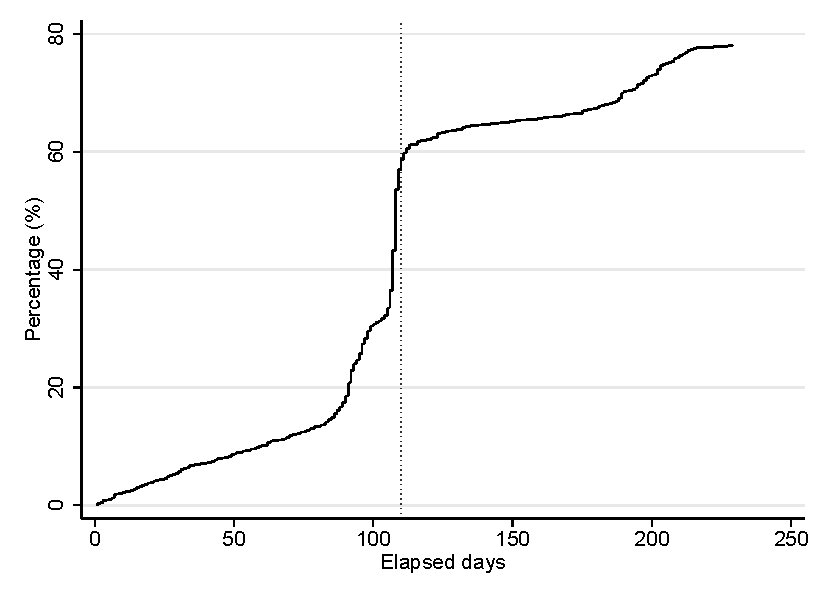
\includegraphics[width=\textwidth]{Figuras/survival_graph_ended.pdf}
    \end{subfigure} 
   \begin{subfigure}{0.49\textwidth}
   \caption{Recovery}
        \centering
        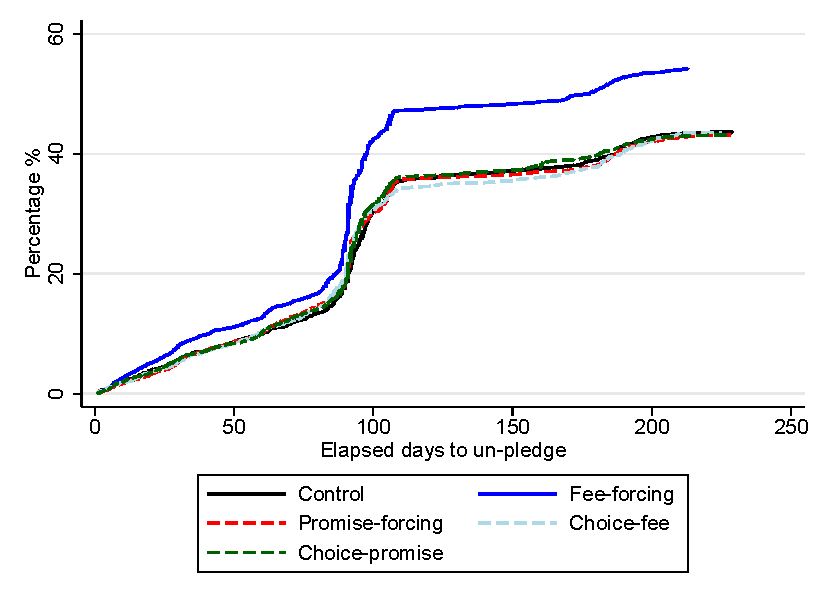
\includegraphics[width=\textwidth]{Figuras/survival_graph_unpledge.pdf}
    \end{subfigure}     
    \end{center}
     \legend{  This Figure shows the CDF of loan completion either default or recovery in Panel (a), or loan recovery in Panel (b), by the number of days since first pawn.}
     %\textit{Do file: }  \texttt{survival\_graph.do}
\end{figure}

\begin{figure}[!htb]
        \caption{\% of payment over time}
    \label{porc_payment_over_time}
    \begin{center}
   \begin{subfigure}{0.49\textwidth}
        \caption{Unconditional}
        \centering
        \includegraphics[width=\textwidth]{Figuras/cumulative_porc_pay_time.pdf}
    \end{subfigure} 
   \begin{subfigure}{0.49\textwidth}
        \caption{Conditional on default}
        \centering
        \includegraphics[width=\textwidth]{Figuras/cumulative_porc_pay_time_default.pdf}
    \end{subfigure}     
    \end{center}
     \legend{  This Figure shows the accumulated percentage of recovery in time by treatment arm. }
     %\textit{Do file: }  \texttt{cumulative\_porc\_pay\_time.do}
\end{figure}


















\section{Alternative explanations}

\subsection{Learning}

Table \ref{learning_table} presents information about borrowers' \emph{future} pawning behavior as a function of treatment assignment. Column (1) considers the 228 clients who returned only a second time to pawn again at a day/branch that was randomly assigned to the choice arm. Each of the two rows in this column presents a difference of mean commitment take-up rates, and associated standard error. The first row compares those who were \emph{initially} assigned to forced commitment against those where were assigned to control; the second row compares those who were initially assigned to the choice commitment arm to those who were assigned to the other two arms. In each case, there is no statistically discernible difference in the rates of commitment take-up. Granted, this is a selected sample because the decision to pawn again is potentially endogenous to the initial treatment allocation. For this reason, Column (2) considers the full sample of 4441 borrowers by re-defining the outcome variable to be an indicator for returning to pawn again at a branch/day when commitment was offered \emph{and} choosing commitment. This composite outcome variable is not subject to the sample selection problem (although it is directly driven by the decision to repeat borrow). The comparison in the two rows remains the same: forced commitment versus control in row one and choice commitment versus forced arms in row two. Again, there is no statistically discernible difference in commitment take-up rates in either row. While these exercises cannot completely exclude the possibility that learning plays a role, they provide no indication that the lack of voluntary compliance is simply a matter of inexperience with commitment.


\begin{table}[!htb]
        \caption{Effect of Prior Assignment on Subsequent Choice}
    \label{learning_table}
\begin{center}
\scriptsize{% Table generated by Excel2LaTeX from sheet 'learning_exp'
\begin{tabular}{lccccccccc}
\toprule
      & \multicolumn{4}{c}{Choose commitment} &       & \multicolumn{4}{c}{Ever chooses commitment} \\
\cmidrule{2-5}\cmidrule{7-10}$t-1$ & (1)   & (2)   & (3)   & (4)   &       & (5)   & (6)   & (7)   & (8) \\
\midrule
\midrule
Forced commitment & -0.0010 & -0.0076 & 0.036 & 0.030 &       & 0.0015 & 0.0043 & 0.0037 & 0.0068 \\
      & (0.044) & (0.058) & (0.036) & (0.053) &       & (0.0032) & (0.0050) & (0.0029) & (0.0047) \\
Choice : Status-quo & -0.032 & -0.026 & -0.054 & -0.054 &       & -0.0021 & -0.0013 & -0.00096 & 0.000025 \\
      & (0.040) & (0.061) & (0.066) & (0.081) &       & (0.0026) & (0.0038) & (0.0023) & (0.0037) \\
Choice : commitment & 0.51*** & 0.35* & 0.40*** & 0.25  &       & 0.031* & 0.027 & 0.026* & 0.023 \\
      & (0.16) & (0.20) & (0.13) & (0.16) &       & (0.016) & (0.019) & (0.014) & (0.018) \\
Default (D) &       & -0.035 &       & -0.024 &       &       & -0.0015 &       & 0.00024 \\
      &       & (0.046) &       & (0.044) &       &       & (0.0037) &       & (0.0034) \\
Forced commitment\#(D) &       & -0.0063 &       & -0.0071 &       &       & -0.0067 &       & -0.0069 \\
      &       & (0.074) &       & (0.077) &       &       & (0.0057) &       & (0.0056) \\
Choice : Status-quo\#(D) &       & -0.0064 &       & -0.034 &       &       & -0.0016 &       & -0.0017 \\
      &       & (0.067) &       & (0.064) &       &       & (0.0045) &       & (0.0044) \\
Choice : commitment\#(D) &       & 0.59*** &       & 0.54*** &       &       & 0.0085 &       & 0.0081 \\
      &       & (0.20) &       & (0.20) &       &       & (0.021) &       & (0.021) \\
Constant & 0.072** & 0.091** & 0.40*** & 0.44*** &       & 0.0046** & 0.0055* & 0.016** & 0.015** \\
      & (0.033) & (0.043) & (0.13) & (0.14) &       & (0.0023) & (0.0029) & (0.0071) & (0.0067) \\
      &       &       &       &       &       &       &       &       &  \\
\midrule
Observations & 240   & 240   & 240   & 240   &       & 4629  & 4629  & 4629  & 4629 \\
R-squared & 0.165 & 0.205 & 0.313 & 0.347 &       & 0.008 & 0.009 & 0.038 & 0.039 \\
Dep var mean & 0.087 &       & 0.087 &       &       & 0.0058 &       & 0.0058 &  \\
Controls &       &       & \checkmark & \checkmark &       &       &       & \checkmark & \checkmark \\
\bottomrule
\bottomrule
\end{tabular}%
}
\end{center}
 \legend{ Column (1) reports results for the 228 borrowers who returned to pawn again at a day/branch that was randomly assigned to the choice arm, enabling us to observe whether they chose commitment or the status quo contract.
Each row presents a difference in mean commitment take-up rates and associated standard errors.
The first row (ATE) compares borrowers who were initially assigned to forced commitment against those were assigned to the control condition.
The second row (ITT) compares borrowers who were initially assigned to the choice commitment condition to those who were not.
Whereas column (1) conditions on the (endogenously) selected sample of borrowers who return to pawn again, column (2) considers the full sample by re-defining the ``outcome'' to be an indicator for whether a borrower pawned again on a day when choice was offered \emph{and} chose commitment.}

%This table explores learning by focusing on a subsample of borrowers in the experiment and observing their subsequent behavior. Column 1 conditions the sample on borrowers who (a) pawned during the experiment a subsequent time after being assigned to control, forced commitment or choice (the regressors), and (b) when pawning again they went to a branch day when (randomly) choice was available, thus enabling us to observe if they chose the commitment contract or the status quo.  in this sample it estimates a linear probability model where the dependent variable is equal to one if the borrower chose the commitment contract in that subsequent `choice' occasion and zero otherwise. The regressors are indicators for the treatment arms in their first pawn in the experiment. Column 1 conditions the sample on the (endogenous) event of pawning again. Column 2 does not condition the sample, but instead defined the dependent variable as equal to one \hl{if the borrower pawned subsequently and choice was available that day and chose commitment, and zero otherwise.}

\end{table}






\subsection{Discount rates}


\begin{figure}[!htb]
        \caption{Financial benefit TUT effect for different discount rates}
    \label{fc_discount_rates}
    \begin{center}
        \centering
        \includegraphics[width=0.55\textwidth]{Figuras/discount_effect_tut.pdf}
    \end{center}
     \legend{ This Figure re-estimates the treatment on the untreated (TUT) effect from Table \ref{tot_tut}, introducing a daily discount factor in the definition of financial benefit. The discount factor reflects time preference, i.e.\ the fact that payments made in the present are more costly for the borrower. At a given annual discount rate in percentage points (x-axis) the solid line gives the adjusted TUT and the shaded regions 90\% \& 95\% confidence bands. A discount factor of one corresponds to the estimate from Table \ref{tot_tut}. For higher discount rates, the adjusted financial cost will be higher, so the financial cost \emph{savings} will be lower. As seen from the figure, borrowers would need to face unrealistically large discount rates to reverse our headline result of a large, positive, and statistically significant TUT effect.}
     %It estimates the effect of the treatment arms  for different discount factors, where a discount factor of 1 corresponds exactly to the estimate of column 1 of Table \ref{main_impact_table}. Because the commitment contract induces earlier payments, this adjusted financial cost will be higher, and thus financial savings will be lower. This figure shows the range of estimated effects and their confidence intervals, where the discount rate used is ploted in the x-axis annualized.    %\textit{Do file: }  \texttt{discounted\_noeffect.do}
\end{figure}





\subsection{Sure Confidence} \label{App_sureconfidence}

\begin{figure}[!htb]
    \caption{Determinants sure confidence}
    \label{determinants_sure}
    \begin{center}
    \begin{subfigure}{0.5\textwidth}
        \centering
        \includegraphics[width=\textwidth]{Figuras/determinants_confidence_100.pdf}
    \end{subfigure}
    \end{center}
     \legend{ The above figure shows the determinants in a bivariate and multivariate OLS regression of sure confidence among the non-choosers. Sure confidence is a binary variable defined to be one when people report a 100\% probability of recovery.}
%\textit{Do file: } \texttt{determinants_sure_confidence.do}       
\end{figure}



\section{Heterogeneity and Bounds}

\subsection{Testing for heterogeneity}
\label{append:chernozhukov}
If the treatment effects $Y_{i1} - Y_{i0}$ are constant across $i$, then we must have
\[
\text{ATE}(X_i) \equiv \mathbbm{E}[Y_{i1} - Y_{i0} |X_i] = \mathbbm{E}[Y_{i1} - Y_{i0}] \equiv \text{ATE}
\]
for any covariates $X_i$ that vary across $i$. If, on the other hand, $\text{ATE}(X_i)$ can be predicted using some scalar function $\tau(\cdot)$ of $X_i$, then the average treatment effect function is not constant so there must be treatment effect heterogeneity. 

We operationalize this idea using a two-step approach proposed by \cite{chernozhukov2018generic}.  We begin by randomly dividing the participants in the forced arms of the experiment ($Z_i \neq 2$) into two groups: a training set and a test set.
These sets are constructed to ensure that all observations from a given branch-day cluster are allocated to the same set.
This avoids inferential problems that could arise from correlated unobservables within clusters.
In the first step, we apply the generalized random forest approach of \cite{atheygrf} to the training set to estimate two proxy predictors: $\psi(\cdot|\text{Training})$ approximates the untreated potential outcome function, $\mathbbm{E}[Y_{i0}|X_i] = \mathbbm{E}[Y_i|Z_i=0,X_i]$, while  $\tau(\cdot|\text{Training})$, approximates the ATE function
\[
\text{ATE}(X_i) = \mathbbm{E}[Y_i|Z_i=1,X_i] - \mathbbm{E}[Y_i|Z_i=0, X_i].
\]
The proxy predictors need not be unbiased or even consistent estimators of the functions they aim to approximate: the goal of this exercise is merely to find a scalar function of $X_i$ that \emph{accurately predicts} $\text{ATE}(X_i)$.
In the second step we fit a linear regression model to data from the training set using regressors constructed from the proxy functions $\psi(\cdot|\text{Training})$ and $\tau(\cdot|\text{Training})$ constructed in the first step. In particular, we estimate 
\begin{equation}
Y_i = \alpha_0 + \alpha_1 \psi_i + \beta_1 (Z_i - \mathbbm{E}[Z_i]) + \beta_2 (Z_i - \mathbbm{E}[Z_i])(\tau_i - \mathbbm{E}[\tau_i]) + \epsilon_i
\label{eq:chernreg}
\end{equation}
where $\psi_i \equiv \psi(X_i|\text{Training})$ and $\tau_i \equiv \tau(X_i|\text{Training})$.\footnote{This is a slightly simpler regression than the one proposed in equation (3.1) of \cite{chernozhukov2018generic}, which involves propensity score weights. Because the random assignment of $Z$ in our experiment does \emph{not} condition on $X$, the propensity score weights in our case are constant over $X$ and hence drop out.} As shown by \cite{chernozhukov2018generic}, the coefficients $\beta_1$ and $\beta_2$ from \eqref{eq:chernreg} identify the \emph{best linear predictor} of the conditional ATE based on $\tau(\cdot|\text{Training})$, namely
\[
\beta_1 = \mathbbm{E}[\text{ATE}(X_i)] = \text{ATE}, \quad
\beta_2 = \frac{\text{Cov}[\text{ATE}(X_i), \tau_i]}{\text{Var}(\tau_i)}.
\]
If treatment effects are homogeneous we must have $\beta_2 = 0$. Rejecting this hypothesis establishes that $\tau_i$ predicts $\text{ATE}(X_i)$ and hence that $\Delta_i$ varies. 
Since $\tau_i$ and $\psi_i$ do not depend on the test set, inference for the regression in \eqref{eq:chernreg} is straightforward conditional on the Training/Test split.  
Our estimate for $\beta_2$ is 2.56 with a one-sided heteroskedasticity-robust (HC3) standard error of 0.43.
Thus we easily reject the null hypothesis of homogeneous treatment effects.



\subsection{Bounds, FOSD and Rank Invariance} \label{bounds_FOSD}



\begin{figure}[!htb]
    \caption{Fan \& Park bounds for benefit in APR\%}
    \label{fan_park_bounds}
    \begin{center}
    \begin{subfigure}{0.5\textwidth}
        \caption{APR}
        \centering
        \includegraphics[width=\textwidth]{Figuras/fan_park_bounds_apr.pdf}
    \end{subfigure}
    \end{center}
        \legend{ This figure depicts the \cite{fan2010sharp} bounds on the distribution $F_\Delta$ of individual treatment effects $\Delta \equiv (Y_1 - Y_0)$, described in Section \ref{sec:bounds}, for the APR outcome.
    The dark red curve and light red shaded region give the estimated upper bound function $\overline{F}$ for $F_\Delta$ and associated (pointwise) 95\% confidence interval. 
    The dark blue curve and light blue shaded region give the estimated lower bound function $\underline{F}$ for $F_\Delta$ and associated (pointwise) 95\% confidence interval.
    Confidence intervals are computed using the asymptotic distribution for the bounds. See \cite{fan2010sharp} for details.
    The bounds are pointwise sharp: at any specified value of $\delta$ the bounds $\underline{F}(\delta) \leq F_\Delta(\delta) \leq \overline{F}(\delta)$ cannot be improved without imposing additional assumptions.
    Evaluating the bounds at $\delta = 0$, we see that between 23\% and 97\% of borrowers have a positive individual treatment effect.
    This is greater than the share of borrowers who chose commitment: 11\%.}
%\textit{Do file: } \texttt{fan\_park\_bnds.do}       
\end{figure}



 
\vspace{.2in}
\begin{figure}[!htb]
        \caption{Empirical CDF: Forced commitment vs Control FOSF}
    \label{ecdf_fc}
    
    \begin{center}
        \begin{subfigure}{0.49\textwidth}
         \caption{APR benefit}
         \centering
         \includegraphics[width=\textwidth]{Figuras/cdf_apr.pdf}
     \end{subfigure} 
   \begin{subfigure}{0.49\textwidth}
        \caption{Financial benefit}
        \centering
        \includegraphics[width=\textwidth]{Figuras/cdf_fc_admin.pdf}
    \end{subfigure} 
    \end{center}
   \legend{  This figure plots the empirical CDF of experimental outcomes separately for the control (status quo) in dashes, and forced commitment contracts (solid). In panel (a), the outcome is APR benefit; in panel (b) the outcome is Financial benefit. 
    The empirical CDF under forced commitment first-order stochastically dominates the empirical CDF under the status quo. This can be seen by examining the dotted line, which shows the difference $(\text{Control} - \text{Commitment})$. }
    %The dotted line at the bottom of panels (a) and (b)   the empirical cumulative distribution function APR and financial cost of financial cost. It does this separately for the fee-forcing contract and for the status-quo contract. The dotted line at the bottom is the difference of the control CDF minus the forced CDF arm. It shows that the CDF of the status quo contract is always below that of the fee-forcing (and this difference is significant for the points indicated by the blue line).
    % \texttt{fosd_ecdf.do}}
\end{figure}
   


\vspace{.2in}
\begin{figure}[!htb]
        \caption{Distribution of treatment effects under rank invariance.}
    \label{te_rankinvariance}
    
    \begin{center}
       \begin{subfigure}{0.49\textwidth}
        \caption{APR benefit}
        \centering
        \includegraphics[width=\textwidth]{Figuras/te_rankinvariance_apr.pdf}
    \end{subfigure} 
   \begin{subfigure}{0.49\textwidth}
        \caption{Financial benefit}
        \centering
        \includegraphics[width=\textwidth]{Figuras/te_rankinvariance_fc_admin.pdf}
    \end{subfigure} 
    \end{center}
    \legend{  This figure shows the CDF of individual treatment effects under the assumption of rank invariance, computed from 
    \[F_\Delta(\delta) = \int_0^1 \mathbbm{1}\{ F_1^{-1}(u) - F_0^{-1}(u)\leq \delta\}\,\mathrm{d}u\]
where $F_1^{-1}$ and $F_0^{-1}$ are the quantile functions of $Y_1$ and $Y_0$.}
    %The dotted line at the bottom of panels (a) and (b)   the empirical cumulative distribution function APR and financial cost of financial cost. It does this separately for the fee-forcing contract and for the status-quo contract. The dotted line at the bottom is the difference of the control CDF minus the forced CDF arm. It shows that the CDF of the status quo contract is always below that of the fee-forcing (and this difference is significant for the points indicated by the blue line).
    % \texttt{te_rankinvariance.do}}
\end{figure}




\section{Derivations for Section \ref{sec:randchoice}}
\label{append:randchoice}


This appendix provides proofs of the results described in Section \ref{sec:randchoice}, using the notation and assumptions described in Section \ref{sec:potentialOutcomes}. 
To simplify the presentation, we omit $i$ subscripts throughout this section.
We also use the shorthand $Z_0 \equiv \mathbbm{1}(Z=0)$, $Z_1 \equiv \mathbbm{1}(Z=1)$, and $Z_2 \equiv\mathbbm{1}(Z=2)$.
For convenience, the following assumption collects our exclusion restriction and the key features of the constrained choice design.

\begin{assumption}\mbox{}
\label{assump:randchoice}
   \begin{enumerate}[(i)]
   \item $Z$ is independent of $(Y_{0}, Y_{1}, C)$
   \item $D = \mathbbm{1}(Z \neq 2)Z + \mathbbm{1}(Z = 2)C$
   \item $Y = \mathbbm{1}(Z = 0) Y_{0} + \mathbbm{1}(Z = 1) Y_{1} + \mathbbm{1}(Z = 2) [ (1 - C) Y_{0} + C Y_{1}]$
   \end{enumerate}
\end{assumption}


\subsection{Point Identification}

We first show that the TOT, TUT, ASB, and ASL effects are point identified under the constrained choice design.
It follows that the ASG effect, $(\text{TOT} - \text{TUT})$, is likewise point identified. 

\begin{lem}
Under Assumption \ref{assump:randchoice},
\label{lem_randchoice}
   \begin{enumerate}[(i)]
       \item $\mathbbm{E}(D|Z=2) = \mathbb{P}(C=1)$
       \item $\mathbbm{E}(Y|Z=0) = \mathbbm{E}(Y_0)$
       \item $\mathbbm{E}(Y|Z=1) = \mathbbm{E}(Y_1)$
       \item $\mathbbm{E}(Y|D=0,Z=2) = \mathbbm{E}(Y_0|C=0)$
       \item $\mathbbm{E}(Y|D=1,Z=2) = \mathbbm{E}(Y_1|C=1)$.
   \end{enumerate} 
\end{lem}

\begin{proof}
Part (i) follows because $Z=2$ implies $D=C$ and $Z$ is independent of $C$.  
Parts (ii) and (iii) follow similarly: given $Z=0$ we have $Y = Y_0$, given $Z=1$ we have $Y = Y_1$, and $Z$ is independent of $(Y_0,Y_1)$.
For parts (iv) and (v), first note that Assumption \ref{assump:randchoice} (iii) implies that $Z$ is conditionally independent of $(Y_0,Y_1)$ given $C$.
Now, $Z=2$ implies that $D=0$ if and only if $C=0$. Hence,
\[
\mathbbm{E}(Y|D=0, Z=2) = \mathbbm{E}(Y_0|D=0, Z=2) = \mathbbm{E}(Y_0|C=0, Z=2)=\mathbbm{E}(Y_0|C=0)
\]
establishing part (iv).
For part (v) $Z=2$ implies that $D=1$ if and only if $C=1$ and hence
\[
\mathbbm{E}(Y|D=1, Z=2) = \mathbbm{E}(Y_1|D=1, Z=2) = \mathbbm{E}(Y_1|C=1, Z=2)= \mathbbm{E}(Y_1|C=1). %\qedhere
\]
\end{proof}

\begin{prop} 
Under Assumption \ref{assump:randchoice},
    \begin{enumerate}[(i)]
        \item $\text{TOT} \equiv \mathbbm{E}(Y_1 - Y_0|C=1)  = \displaystyle \frac{\mathbbm{E}(Y|Z=2) - \mathbbm{E}(Y|Z=0)}{\mathbbm{E}(D|Z=2)}$
        \item $\text{TUT} \equiv \mathbbm{E}(Y_1 - Y_0|C=0) = \displaystyle \frac{\mathbbm{E}(Y|Z=1) - \mathbbm{E}(Y|Z=2)}{1 - \mathbbm{E}(D|Z=2)}$
        \item $\text{ASB} \equiv \mathbbm{E}(Y_0|C=1) - \mathbbm{E}(Y_0|C=0) = \displaystyle \frac{\mathbbm{E}(Y|Z=0) - \mathbbm{E}(Y|Z=2,D=0)}{\mathbbm{E}(D|Z=2)}$
        \item $\text{ASL} \equiv \mathbbm{E}(Y_1|C=1) - \mathbbm{E}(Y_1|C=0) = \displaystyle \frac{\mathbbm{E}(Y|Z=2,D=1) - \mathbbm{E}(Y|Z=1)}{1 - \mathbbm{E}(D|Z=2)}$.
    \end{enumerate}
\end{prop}

\begin{proof}
For parts (i) and (iii) we require an expression for $\mathbbm{E}(Y_0|C=1)$ in terms of the observables $(Y, D, Z)$.
By Lemma \ref{lem_randchoice}(ii) and iterated expectations 
\[
\mathbbm{E}(Y|Z=0) = \mathbbm{E}(Y_0) = \mathbbm{E}(Y_0|C=0) \mathbbm{P}(C=0) + \mathbbm{E}(Y_0|C=1) \mathbbm{P}(C=1).
\]
Re-arranging and substituting Lemma \ref{lem_randchoice}(i) and (iv),
\begin{align}
\mathbbm{E}(Y_0|C=1)  &= \frac{\mathbbm{E}(Y|Z=0) - \mathbbm{E}(Y_0|C=0) \mathbbm{P}(C=0)}{\mathbbm{P}(C=1)}\nonumber\\ 
&=  \frac{\mathbbm{E}(Y|Z=0) - \mathbbm{E}(Y|Z=2,D=0) \mathbbm{E}(1 - D|Z=2)}{\mathbbm{E}(D|Z=2)}.
\label{eq:Y0C1}
\end{align}
Part (i) follows by combining \eqref{eq:Y0C1} with Lemma \ref{lem_randchoice}(v) and simplifying; part (iii) follows by combining \eqref{eq:Y0C1} with Lemma \ref{lem_randchoice}(iv) and simplifying.
Similarly, for parts (ii) and (iv) we require an expression for $\mathbbm{E}(Y_1|C=0)$ in terms of observables.
By Lemma \ref{lem_randchoice}(iii) and iterated expectations,
\[
\mathbbm{E}(Y|Z=1) = \mathbbm{E}(Y_1) = \mathbbm{E}(Y_1|C=0)\mathbbm{P}(C=0) + \mathbbm{E}(Y_1|C=1) \mathbbm{P}(C=1).
\]
Re-arranging and substituting Lemma \ref{lem_randchoice}(i) and (v),
\begin{align}
\mathbbm{E}(Y_1|C=0) 
&= \frac{\mathbbm{E}(Y|Z=1) - \mathbbm{E}(Y_1|C=1)\mathbbm{P}(C=1)}{\mathbb{P}(D=0)} \nonumber\\
&=\frac{\mathbbm{E}(Y|Z=1) - \mathbbm{E}(Y|Z=2,D=1)\mathbbm{E}(D|Z=2)}{\mathbb{E}(1-D|Z=2)}.
\label{eq:Y1C0}
\end{align}
Part (ii) follows by combining \eqref{eq:Y1C0} with Lemma \ref{lem_randchoice}(iv) and simplifying; part (iv) follows by combining \eqref{eq:Y1C0} with Lemma \ref{lem_randchoice}(v) and simplifying.
\end{proof}

\subsection{Regression-based Estimation of TOT, TUT, ASG, ASL, and ASB}

We now show how a collection of just-identified, linear IV regressions can be used to consistently estimate the ATE, TOT, and TUT effects, along with each of the ingredients needed to construct the ASL and ASB. 
These results are used below to provide a recipe for cluster-robust inference for the ASG, ASL, and ASB effects.
The first result provides a regression-based approach to estimate the ATE and TOT.

\begin{prop} 
\label{prop:TOTreg}
Under Assumption \ref{assump:randchoice},
\[
Y = \mathbbm{E}(Y_0) + \text{ATE}\times Z_1 + \text{TOT} \times Z_2 D + U
\]
where $\mathbb{E}(U|Z) = 0$.
Therefore, under standard regularity conditions, an IV regression of $Y$ on an intercept, $Z_1$ and $Z_2 D$ with instruments $(1, Z_0, Z_1)$ provides a consistent estimator of the ATE and TOT effects.
\end{prop}

\begin{proof}
By Assumption \ref{assump:randchoice} (iii),
\begin{align*}
Y &= Z_0 Y_0 + Z_1 Y_1 + Z_2[(1 - C) Y_0 + CY_1]\\
&= (Z_0 + Z_2)Y_0 + Z_1 Y_1 + Z_2C(Y_1 - Y_0)\\
&= (Z_0 + Z_1 + Z_2)Y_0 + Z_1 (Y_1 - Y_0) + Z_2D(Y_1 - Y_0)\\
&= Y_0 + Z_1 (Y_1 - Y_0) + Z_2D(Y_1 - Y_0).
\end{align*}
since $Z_2 D = Z_2 C$ and $(Z_0 + Z_1 + Z_2) = 1$.
Thus, defining 
\[
U \equiv [Y_0 - \mathbbm{E}(Y_0)] + Z_1[(Y_1 - Y_0) - \text{ATE}] + Z_2 D[(Y_1 - Y_0) - \text{TOT}]
\]
by construction we have
\[
Y = \mathbbm{E}(Y_0) + \text{ATE} \times Z_1 + \text{TOT} \times Z_2 D+ U.
\]
Now, since $Z_2 D = Z_2 C$ and $Z$ is independent of $(Y_1, Y_0)$ by Assumption \ref{assump:randchoice} (i), we have
\begin{align*}
\mathbbm{E}(U|Z) &= [\mathbbm{E}(Y_0|Z) - \mathbbm{E}(Y_0)]  + Z_1[\mathbbm{E}(Y_1 - Y_0|Z) - \text{ATE}] +  \mathbbm{E}\left[Z_2 D\left\{(Y_1 - Y_0) - \text{TOT}\right\}|Z\right]\\
&= [\mathbbm{E}(Y_0) - \mathbbm{E}(Y_0)]  + Z_1[\mathbbm{E}(Y_1 - Y_0) - \text{ATE}] + Z_2 \mathbbm{E}\left[C\left\{(Y_1 - Y_0) - \text{TOT}\right\}|Z\right]\\
&= Z_2 \mathbbm{E}\left[C\left\{(Y_1 - Y_0) - \text{TOT}\right\}|Z\right].
\end{align*}
Finally, by iterated expectations
\begin{align*}
\mathbbm{E}\left[C\left\{(Y_1 - Y_0) - \text{TOT}\right\}|Z\right] &=  \mathbbm{P}(C=1|Z) \left[\mathbbm{E}(Y_1 - Y_0|C=1,Z)  - \text{TOT}\right]\\
&= \mathbbm{P}(C=1)\left[\mathbbm{E}(Y_1 - Y_0|C=1) - \text{TOT} \right]=0
\end{align*}
since $Z$ is conditionally independent of $(Y_0, Y_1)$ given $C$, an implication of \ref{assump:randchoice} (i).
\end{proof}

The next proposition provides regression-based estimates of the ATE and TUT.
\begin{prop}
\label{prop:TUTreg}
Under Assumption \ref{assump:randchoice}
\[
Y = \mathbbm{E}(Y_1) + \text{ATE}\times -Z_0 + \text{TUT} \times -Z_2 (1 - D) + V
\] 
where $\mathbb{E}(V|Z) = 0$.
Therefore, under standard regularity conditions, an IV regression of $Y$ on an intercept, $-Z_0$ and $-Z_2(1-D)$ with instruments $(1, Z_0, Z_1)$ provides consistent estimates of the ATE and TUT effects.
\end{prop}

\begin{proof}
By Assumption \ref{assump:randchoice} (iii),
\begin{align*}
Y &= Z_0 Y_0 + Z_1 Y_1 + Z_2[(1 - C) Y_0 + CY_1]\\
&= Z_0 Y_0 + Z_1 Y_1 + Z_2[(1 - C) (Y_0 - Y_1) + Y_1]\\
&= Z_0 Y_0 + (Z_1 + Z_2) Y_1 + Z_2(1 - C) (Y_0 - Y_1) \\
&= Z_0 Y_0 + (1 - Z_0) Y_1 + Z_2(1 - D) (Y_0 - Y_1) \\
&= Y_1 - Z_0 (Y_1 - Y_0) - Z_2(1 - D) (Y_1 - Y_0)
\end{align*}
since $Z_2(1 - C)= Z_2(1 - D)$ and $(Z_1 + Z_2) = 1 - Z_0$.
Thus, defining 
\[
V \equiv [Y_1 - \mathbb{E}(Y_1)] - Z_0[(Y_1 - Y_0) - \text{ATE}] - Z_2(1 - D)[(Y_1 - Y_0) - \text{TUT}]
\]
by construction we have
\[
Y = \mathbb{E}(Y_1) + \text{ATE} \times -Z_0 + \text{TUT} \times -Z_2(1 - D) + V.
\]
Now, since $Z_2(1 - D) = Z_2 (1 - C)$ and $Z$ is independent of $(Y_0, Y_1)$ by Assumption \ref{assump:randchoice} (i),
\begin{align*}
\mathbb{E}(V|Z) &= [\mathbb{E}(Y_1|Z) - \mathbb{E}(Y_1)] - Z_0[\mathbb{E}(Y_1 - Y_0|Z) - \text{ATE}] - \mathbb{E}[Z_2(1 - D)\left\{(Y_1 - Y_0) - \text{TUT}\right\}|Z]\\
&= [\mathbb{E}(Y_1) - \mathbb{E}(Y_1)] - Z_0[\mathbb{E}(Y_1 - Y_0) - \text{ATE}] - Z_2\mathbb{E}[(1 - C)\left\{(Y_1 - Y_0) - \text{TUT}\right\}|Z]\\
&= -Z_2\mathbb{E}[(1 - C)\left\{(Y_1 - Y_0) - \text{TUT}\right\}|Z].
\end{align*}
Finally, by iterated expectations,
\begin{align*}
\mathbb{E}[(1 - C)\left\{(Y_1 - Y_0) - \text{TUT}\right\}|Z]&= \mathbb{P}(C=0|Z)\left[ \mathbb{E}(Y_1 - Y_0|C=0, Z) - \text{TUT}\right]\\
&= \mathbb{P}(C=0|Z) \left[ \mathbb{E}(Y_1 - Y_0|C=0) - \text{TUT}\right] = 0
\end{align*}
since $Z$ is conditionally independent of $(Y_0, Y_1)$ given $C$, an implication of Assumption \ref{assump:randchoice} (i).
\end{proof}

Since $\text{ASG} = \text{TOT} - \text{TUT}$, the preceding two propositions provide consistent estimates of $\text{ASG}$ effect.
The $\text{ASB}$ effect, $\mathbbm{E}(Y_0|C=1) - \mathbb{E}(Y_0|C=0)$, can likewise be estimated by taking the difference of coefficients across two linear IV regressions, as shown in the following proposition.

\begin{prop}
\label{prop:ASBreg}
Under Assumption \ref{assump:randchoice}
\begin{align}
\label{eq:ASB0}
    (1 - D) Y &= \mathbbm{E}(Y_{0}) \times Z_0 + \mathbbm{E}(Y_{0}|C=0) \times (1 - D)Z_2 + U_{0}\\
\label{eq:ASB1}
    (1 - D) Y &= \mathbbm{E}(Y_{0}) \times(Z_0 + Z_2) + \mathbbm{E}(Y_{0}|C=1)\times -DZ_2 + U_{1}
\end{align}
where $\mathbbm{E}(U_0|Z) = \mathbbm{E}(U_1|Z) = 0$.
Thus, under standard regularity conditions, an IV regression of $(1 - D)Y$ on $Z_0$ and $(1 - D)Z_2$ with instruments $(Z_0, Z_2)$ and no intercept provides consistent estimates of $\mathbb{E}(Y_0)$ and $\mathbb{E}(Y_0|C=0)$. 
Similarly, an IV regression of $(1 - D)Y$ on $(Z_0 + Z_2)$ and $-DZ_2$ with instruments $(Z_0, Z_2)$ and no intercept provides consistent estimates of $\mathbb{E}(Y_0)$ and $\mathbb{E}(Y_0|C=1)$.
\end{prop}

\begin{proof}
Assumption \ref{assump:randchoice} (ii) implies $(1 - D) = Z_0 + Z_2(1 - C)$. Hence, by Assumption \ref{assump:randchoice} (iii),
\begin{align*}
(1 - D)Y &=  [Z_0 + Z_2 (1 - C)]\left\{Z_0 Y_0 + Z_1 Y_1 + Z_2[(1 - C) Y_0 + CY_1]\right\}\\
&= Z_0 Y_0 + Z_2 (1 - C) [(1 - C) Y_0 + C Y_1]\\
&= Z_0 Y_0 + Z_2 (1 - C) Y_0.
\end{align*}
because $Z_j^2 = Z_j$ for any $j$ and $Z_j Z_k = 0$ for any $j \neq k$ and, similarly, $(1 - C)^2 = (1 - C)$ and $C (1 - C) = 0$.
Therefore, since $Z_2 (1 - C) = Z_2 (1 - D)$,
\begin{align*}
(1 - D)Y &= Z_0 Y_0 + Z_2 (1 - D) Y_0\\
(1 - D)Y &= (Z_0 + Z_2) Y_0 + (-DZ_2) Y_0. 
\end{align*}
Now, defining
\begin{align*}
U_0 &\equiv Z_0 [Y_0 - \mathbbm{E}(Y_0)] + Z_2(1 - D)[Y_0 - \mathbbm{E}(Y_0|C=0)]\\
U_1 &\equiv (Z_0 + Z_2)[Y_0 - \mathbbm{E}(Y_0)] + (-Z_2 D)[Y_0 - \mathbbm{E}(Y_0|C=1)]
\end{align*}
by construction, we have
\begin{align*}
Y &= \mathbbm{E}(Y_0) \times Z_0 + \mathbbm{E}(Y_0|C=0) \times Z_2(1 - D) + U_0\\
Y &= \mathbbm{E}(Y_0) \times (Z_0 + Z_2)+ \mathbbm{E}(Y_0|C=1) (-Z_2D) + U_1.
\end{align*}
Finally, since $Z_2(1-D) = Z_2(1 - C)$, and $Z$ is independent of $Y_0$,  
\begin{align*}
\mathbbm{E}(U_0|Z) &= Z_0[\mathbbm{E}(Y_0|Z) - \mathbbm{E}(Y_0)] + Z_2\mathbbm{E}\{(1 - C) [Y_0 - \mathbbm{E}(Y_0|C=0) |Z\}\\
&= Z_2 \mathbbm{E}[Y_0 - \mathbbm{E}(Y_0|C=0) | C = 0, Z] = 0
\end{align*}
where the final two steps follow by iterated expectations and the fact that  $Z$ is conditionally independent of $Y_0$ given $C$. 
Since $Z_2 D = Z_2 C$, a nearly identical argument gives
\begin{align*}
\mathbbm{E}(U_1|Z) &= (Z_0 + Z_2)[Y_0 - \mathbbm{E}(Y_0|Z)] -Z_2\mathbbm{E}\{C [Y_0 - \mathbbm{E}(Y_0|C=1) |Z\}\\
&= -Z_2 \mathbbm{E}[Y_0 - \mathbbm{E}(Y_0|C=0) | C = 1, Z] = 0. \qedhere
\end{align*}
\end{proof}


The next results shows that the $\text{ASL}$ effect, $\mathbbm{E}(Y_1|C=1) - \mathbb{E}(Y_1|C=0)$, can be estimated as the difference of coefficients across two linear IV regressions, as shown in the following proposition.

\begin{prop}
\label{prop:ASLreg}
Under Assumption \ref{assump:randchoice},
\begin{align}
\label{eq:ASL0}
    D Y &= \mathbbm{E}(Y_{1}) \times(Z_1 + Z_2) + \mathbbm{E}(Y_{1}|C=0)\times (D - 1)Z_2 + V_{0}\\
\label{eq:ASL1}
    D Y &= \mathbbm{E}(Y_{1}) \times Z_1 + \mathbbm{E}(Y_{1}|C=1)\times D Z_2+ V_{1}
\end{align}
where $\mathbbm{E}(V_0|Z) = \mathbbm{E}(V_1|Z) = 0$.
Thus, under standard regularity conditions, an IV regression of $DY$ on $(Z_1 + Z_2)$ and $-Z_2(1 - D)$ with instruments $(Z_1, Z_2)$ and no intercept provides consistent estimates of $\mathbb{E}(Y_1)$ and $\mathbb{E}(Y_1|C=1)$.
Similarly, an IV regression of $DY$ on $Z_1$ and $DZ_2$ with instruments $(Z_1, Z_2)$ and no intercept provides consistent estimates of $\mathbb{E}(Y_1)$ and $\mathbb{E}(Y_1|C=1)$. 
\end{prop}


\begin{proof}
By Assumption \ref{assump:randchoice}, $D = Z_1 + Z_2 C$. Hence, by Assumption \ref{assump:randchoice} (iii),
\begin{align*}
DY &=  (Z_1 + Z_2 C)\left\{Z_0 Y_0 + Z_1 Y_1 + Z_2[(1 - C) Y_0 + CY_1]\right\}\\
&= Z_1 Y_1 + Z_2 C[(1 -C) Y_0 + C Y_1]\\
&= Z_1 Y_1 + Z_2 C Y_1
\end{align*}
because $Z_j^2 = Z_j$ for any $j$ and $Z_j Z_k = 0$ for any $j \neq k$ and, similarly, $(1 - C)^2 = (1 - C)$ and $C (1 - C) = 0$. Therefore, since $Z_2 (1 - C) = Z_2 (1 - D)$,
\begin{align*}
 DY &= (Z_1 + Z_2)Y_1 + Z_2 (D - 1) Y_1\\
 DY &= Z_1 Y_1 + Z_2 D Y_1.
\end{align*}
Now, defining
\begin{align*}
V_0 &= (Z_1 + Z_2)[Y_1 - \mathbbm{E}(Y_1)] + Z_2(D - 1)[Y_1 - \mathbbm{E}(Y_1|C=0)]\\
V_1 &= Z_1[Y_1 - \mathbbm{E}(Y_1)] + Z_2D[Y_1 - \mathbbm{E}(Y_1|C=1)]
\end{align*}
by construction we have
\begin{align*}
Y &= \mathbbm{E}(Y_1) \times (Z_1 + Z_2) + \mathbbm{E}(Y_1 | C = 0) \times Z_2 (D - 1) + V_0\\
Y &= \mathbbm{E}(Y_1) \times Z_1 + \mathbbm{E}(Y_1 | C = 1) \times Z_2 D + V _1.
\end{align*}
Finally, since $Z_2(1 - D) = Z_2(1 - C)$ and $Z$ is independent of $Y_1$,
\begin{align*}
\mathbbm{E}(V_0|Z) &= (Z_1 + Z_2) [\mathbbm{E}(Y_1|Z) - \mathbbm{E}(Y_1) ]  - Z_2 \mathbbm{E}\{(1 - C)  [Y_1 - \mathbbm{E}(Y_1 | C=0)|Z\} \\
&= -Z_2 \mathbbm{E}[Y_1 - \mathbbm{E}(Y_1 | C=0)|C=0, Z] = 0
\end{align*}
where the final two steps follow by iterated expectations and the fact that  $Z$ is conditionally independent of $Y_1$ given $C$. 
Since $Z_2 D = Z_2 C$, a nearly identical argument gives
\begin{align*}
\mathbbm{E}(V_1|Z) &= Z_1 [\mathbbm{E}(Y_1 | Z) - \mathbbm{E}(Y_1)]  + Z_2 \mathbbm{E}\{C  [Y_1 - \mathbbm{E}(Y_1 | C=1)|Z\} \\
&= Z_2 \mathbbm{E}[Y_1 - \mathbbm{E}(Y_1 | C=1)|C=1, Z] = 0. \qedhere
\end{align*}
\end{proof}




\subsection{Inference for ASG, ASB, and ASL}
\label{subsec:inference}
We now explain how to carry out cluster-robust inference for the ASG, ASB, and ASL effects, as implemented in our companion STATA package.
Each of these effects can be expressed as a difference of coefficients from two just-identified linear IV regressions.
The ASG effect is the difference of the \text{TOT} effect from Proposition \ref{prop:TOTreg} and the \text{TUT} effect from Proposition \ref{prop:TUTreg}.
Similarly, the ASB effect is the difference of $\mathbb{E}(Y_0|C=1)$ and $\mathbbm{E}(Y_0|C=0)$ from Proposition \ref{prop:ASBreg} while the ASL effect is the difference of $\mathbbm{E}(Y_1|C=1)$ and $\mathbbm{E}(Y_1|C=0)$ from Proposition \ref{prop:ASLreg}.
Within each pair of IV regressions the outcome variable and instrument set is identical; only the regressors differ. 
Since our estimators of all three effects share the same structure, our discussion of inference abstracts from the specific regressors and instruments used in each case to avoid duplication. 
To implement these results in practice without relying on our STATA package, simply substitute supply the regressors and instruments specified in the relevant propositions. 

Let $g = 1, ..., G$ index clusters and $i = 1, ..., N_g$ index individuals within a particular cluster $g$. 
In our experiment, a cluster is a branch-day combination and the experimentally-assigned treatment (control, forced, or choice arm) is assigned at the cluster level.
We assume that observations are iid across clusters but potentially correlated within cluster.
Now consider a pair of just-identified linear IV regressions given by
\begin{align*}
Y_{ig} &= \boldsymbol{X}_{1,ig}' \boldsymbol{\theta}_0 + U_{ig} \\
Y_{ig} &= \boldsymbol{X}_{0,ig}' \boldsymbol{\theta}_1 + V_{ig}
\end{align*}
with common instrument vector $\boldsymbol{W}_{ig}$. 
Stacking observations in the usual manner, e.g.\
\[
\mathbf{W}_g \equiv \begin{bmatrix}
\boldsymbol{W}_{1g}' \\
\vdots \\
\boldsymbol{W}_{N_gg}' \\
\end{bmatrix}, \quad
\mathbf{W} = \begin{bmatrix}
\mathbf{W}_1\\ \vdots \\ \mathbf{W}_G
\end{bmatrix},
\]
we can write the preceding equations in matrix form as
\begin{align*}
\mathbf{Y} &= \mathbf{X}_1\boldsymbol{\theta_1} + \mathbf{U}\\
\mathbf{Y} &= \mathbf{X}_0\boldsymbol{\theta_0} + \mathbf{V}
\end{align*}
with instrument matrix $\mathbf{W}$.
Now, the IV estimators for $\boldsymbol{\theta}_1$ and $\boldsymbol{\theta}_0$ can be expressed as 
\begin{align*}
\widehat{\boldsymbol{\theta}}_1 
&= \left(\mathbf{W}'\mathbf{X}_1\right)^{-1}\mathbf{W}'\mathbf{Y}  = \boldsymbol{\theta}_1 + \left(\mathbf{W}'\mathbf{X}_1\right)^{-1}\mathbf{W}'\mathbf{U}\\ 
\widehat{\boldsymbol{\theta}}_0 
&= \left(\mathbf{W}'\mathbf{X}_0\right)^{-1}\mathbf{W}'\mathbf{Y} = \boldsymbol{\theta}_0 + \left(\mathbf{W}'\mathbf{X}_0\right)^{-1}\mathbf{W}'\mathbf{V}.
\end{align*}
Our parameter of interest is an element of the difference $(\theta_1 - \theta_0)$, so  it suffices to calculate the asymptotic distribution of $(\widehat{\boldsymbol{\theta}}_1 - \widehat{\boldsymbol{\theta}}_0)$.

Re-arranging the preceding two equations, we have
\begin{align*}
\sqrt{G} \left(\widehat{\boldsymbol{\theta}}_1  - \boldsymbol{\theta}_1\right) &= 
 \left(\frac{\mathbf{W}'\mathbf{X}_1}{G}\right)^{-1}\left(\frac{\mathbf{W}'\mathbf{U}}{\sqrt{G}}\right) = \left( \frac{1}{G} \sum_{g=1}^G \mathbf{W}_g' \mathbf{X}_{1,g}\right)^{-1}\left(\frac{1}{\sqrt{G}} \sum_{g=1}^G\mathbf{W}_g' \mathbf{U}_g\right) \\ 
\sqrt{G} \left(\widehat{\boldsymbol{\theta}}_0  - \boldsymbol{\theta}_0\right) &= 
 \left(\frac{\mathbf{W}'\mathbf{X}_0}{G}\right)^{-1}\left(\frac{\mathbf{W}'\mathbf{V}}{\sqrt{G}}\right) = \left( \frac{1}{G} \sum_{g=1}^G \mathbf{W}_g' \mathbf{X}_{0,g}\right)^{-1}\left(\frac{1}{\sqrt{G}} \sum_{g=1}^G\mathbf{W}_g' \mathbf{V}_g\right).
\end{align*}
Now, define $\mathbf{Q}_0 \equiv \mathbb{E}[\mathbf{W}_g'\mathbf{X}_{0g}]$ and $\mathbf{Q}_1 \equiv \mathbb{E}[\mathbf{W}_g'\mathbf{X}_{1g}]$ and suppose that these expectations exist and that the matrices $\mathbf{Q}_0$ and $\mathbf{Q}_1$ are invertible. Then, as $G \rightarrow \infty$
\[
 \left( \frac{1}{G} \sum_{g=1}^G \mathbf{W}_g' \mathbf{X}_{0,g}\right)^{-1} \rightarrow_p \mathbf{Q}_0^{-1}, \quad
 \left( \frac{1}{G} \sum_{g=1}^G \mathbf{W}_g' \mathbf{X}_{1,g}\right)^{-1} \rightarrow_p \mathbf{Q}_1^{-1} \quad
\]
by the continuous mapping theorem.
Now, by our experimental design and exclusion restriction, $\mathbf{W}_{ig}$ is independent of $U_{ig}$ both unconditionally and conditional on cluster size. 
Therefore,
\begin{align*}
\mathbb{E}[\mathbf{W}_g' \mathbf{U}_g] &=  \mathbb{E}\left[ \sum_{i=1}^{N_g} \mathbf{W}_{ig} U_{ig} \right] = \mathbb{E}_{N_g}\left[ \mathbb{E}\left\{\left. \sum_{i=1}^{N_g} \mathbf{W}_{ig} U_{ig} \right| N_g \right\}\right]\\
&= \mathbb{E}_{N_g}\left[ \sum_{i=1}^{N_g} \mathbb{E}(\mathbf{W}_{ig} U_{ig}|N_g)\right] = \mathbb{E}_{N_g}\left[ \sum_{i=1}^{N_g} \mathbb{E}(\mathbf{W}_{ig}U_{ig})\right] = 0
\end{align*}
by iterated expectations, and similarly smilarly, $\mathbb{E}[\mathbf{W}_g'\mathbf{V}_g] = \mathbf{0}$. 
Thus, under mild regularity conditions (e.g.\ finite fourth moments), as $G \rightarrow \infty$  we have
\[
\frac{1}{\sqrt{G}} \sum_{g=1}^G \mathbf{W}_g' \otimes \begin{bmatrix} \mathbf{U}_g \\ \mathbf{V}_g \end{bmatrix} \rightarrow_d \text{N}(\mathbf{0}, \boldsymbol{\Omega})
\]
where the heteroskedasticity-- and cluster--robust variance-covariance matrix $\boldsymbol{\Omega}$ is defined as
\[
\boldsymbol{\Omega} \equiv 
 \mathbb{E} \left[\left(\mathbf{W}_g \mathbf{W}_g' \right)\otimes \begin{pmatrix}
\mathbf{U}_g \mathbf{U}_g' & \mathbf{U}_g \mathbf{V}_g' \\
\mathbf{V}_g \mathbf{U}_g' & \mathbf{V}_g \mathbf{V}_g'  
\end{pmatrix} \right] \equiv \begin{bmatrix}
\Omega_{UU} & \Omega_{UV} \\
\Omega_{VU} & \Omega_{VV}
\end{bmatrix}.
\]
Therefore, the joint limiting distribution of $\widehat{\boldsymbol{\theta}}_1$ and $\widehat{\boldsymbol{\theta}}_0$ is given by
\[
\begin{bmatrix}
\sqrt{G}(\widehat{\boldsymbol{\theta}}_1 - \boldsymbol{\theta}_1)\\
\sqrt{G}(\widehat{\boldsymbol{\theta}}_0 - \boldsymbol{\theta}_0)
\end{bmatrix} \rightarrow_d
\begin{bmatrix}
\mathbf{Q}_1^{-1} & \mathbf{0} \\
\mathbf{0} & \mathbf{Q}_0^{-1} 
\end{bmatrix}
\begin{bmatrix}
\boldsymbol{\xi}_U \\ \boldsymbol{\xi}_V 
\end{bmatrix}, \quad
\begin{bmatrix}
\boldsymbol{\xi}_U \\ \boldsymbol{\xi}_V 
\end{bmatrix} \sim \text{N}\left(\begin{bmatrix} \mathbf{0} \\ \mathbf{0}\end{bmatrix},
\begin{bmatrix}
\Omega_{UU} & \Omega_{UV} \\
\Omega_{VU} & \Omega_{VV}
\end{bmatrix}\right)
\]
from which it follows by the continuous mapping theorem that
\[
\sqrt{G}\left[ (\widehat{\boldsymbol{\theta}}_1 - \widehat{\boldsymbol{\theta}}_0 ) - (\boldsymbol{\theta}_1 - \boldsymbol{\theta}_0)\right] 
\rightarrow_d
\begin{bmatrix}
\mathbf{Q}_1^{-1} & -\mathbf{Q}_0^{-1}
\end{bmatrix}
\begin{bmatrix}
\boldsymbol{\xi}_U \\ \boldsymbol{\xi}_V 
\end{bmatrix}.
\]
To use this result in practice, we estimate the standard errors of  $(\widehat{\boldsymbol{\theta}}_1 - \widehat{\boldsymbol{\theta}}_0)$ as the square root of the diagonal elements of the matrix
\[
\widehat{\text{Avar}}(\widehat{\boldsymbol{\theta}}_1 - \widehat{\boldsymbol{\theta}}_0) 
= \begin{bmatrix}
\left(\mathbf{W}'\mathbf{X}_1\right)^{-1} &
-\left(\mathbf{W}'\mathbf{X}_0\right)^{-1} 
\end{bmatrix}
\begin{bmatrix}
\mathbf{S}_{UU}& \mathbf{S}_{UV}\\
\mathbf{S}_{VU}& \mathbf{S}_{VV}
\end{bmatrix} 
\begin{bmatrix}
\left(\mathbf{X}_1'\mathbf{W}\right)^{-1} \\
-\left(\mathbf{X}_0'\mathbf{W}\right)^{-1} 
\end{bmatrix}
\]
where
\begin{align*}
\mathbf{S}_{UU} &\equiv \sum_{g=1}^G \mathbf{W}_g' \widehat{\mathbf{U}}_g \widehat{\mathbf{U}}_g' \mathbf{W}_g\\
\mathbf{S}_{UV} &\equiv \sum_{g=1}^G \mathbf{W}_g' \widehat{\mathbf{U}}_g \widehat{\mathbf{V}}_g' \mathbf{W}_g\\
\mathbf{S}_{VU} &\equiv \mathbf{S}_{UV}'\\
\mathbf{S}_{VV} &\equiv \sum_{g=1}^G \mathbf{W}_g' \widehat{\mathbf{V}}_g \widehat{\mathbf{V}}_g' \mathbf{W}_g
\end{align*}
and we define the IV residuals
\begin{align*}
\widehat{\mathbf{U}}_g &\equiv \mathbf{Y}_g - \mathbf{X}_{1,g}\widehat{\boldsymbol{\theta}}_1\\
\widehat{\mathbf{V}}_g &\equiv \mathbf{Y}_g - \mathbf{X}_{0,g}\widehat{\boldsymbol{\theta}}_0.
\end{align*}
In our application the number of clusters, $G$, is large.
If desired, an \emph{ad hoc} degrees of freedom correction can be applied by multiplying the standard errors by $\sqrt{G/(G-1)}$.


\section{Testable Implications of the Exclusion Restriction}
\label{append:exclusion}

\normalsize
\linespread{1.25}
%Really force it to normal size and linespread
\normalsize
\linespread{1.25}

This section describes the testable implications of our exclusion restrictions: \eqref{eq:exclusion0} and \eqref{eq:exclusion1} from Section \ref{sec:potentialOutcomes}. 
To consider possible violations of these conditions, it is helpful to introduce some additional notation.
As above, let $Y_0 \equiv Y(d=0,z=0)$ and $Y_1 \equiv Y(d=1,z=1)$ denote the potential outcomes under \emph{forced treatment}: $Y_0$ is the potential outcome when forced into the status quo contract and $Y_1$ when forced into the commitment contract. 
Further let $Y_{0,2} \equiv Y(d=0,z=2)$ and $Y_{1,2} \equiv Y(d=1,z=2)$ denote the potential outcomes under \emph{free choice of treatment}: $Y_{0,2}$ is the potential outcome when choosing the status quo contract and $Y_{1,2}$ when choosing the commitment contract. 
Using this notation, \eqref{eq:exclusion0} becomes $Y_0 = Y_{0,2}$ and while \eqref{eq:exclusion1} becomes $Y_1 = Y_{1,2}$.
If we do not impose this pair of equalities, part (iii) of Assumption \ref{assump:randchoice} becomes 
\[
Y = \mathbbm{1}(Z =0) Y_{0} + \mathbbm{1}(Z = 1)  Y_{1}  + \mathbbm{1}(Z = 2) \left[(1 - C) Y_{0,2} + C Y_{1,2} \right]
\]
but parts (i) and (ii) continue to hold.
Accordingly, parts (i)--(iii) of Lemma \ref{lem_randchoice} are unchanged, while parts (iv) and (v) become
\[
\mathbbm{E}(Y|D=0,Z=2) = \mathbbm{E}(Y_{0,2}|C=0), \quad
\mathbbm{E}(Y|D=1,Z=2) = \mathbbm{E}(Y_{0,1}|C=1).
\]
Using these expressions, the testable restrictions we consider here are as follows:
\begin{align}
\label{eq:exclusion_append0}
\mathbbm{E}(Y_0|C=0) &= \mathbbm{E}(Y_{0,2}|C=0) \\
\label{eq:exclusion_append1}
\mathbbm{E}(Y_1|C=1) &= \mathbbm{E}(Y_{1,2}|C=1).
\end{align}
Equation \ref{eq:exclusion_append0} is a restriction on the average potential outcomes of non-choosers that we use to point identify the TUT effect.
It says that someone who \emph{would} choose the control condition when given a choice, experiences the same potential outcome, on average, when \emph{assigned} to the control condition.
Equation \ref{eq:exclusion_append1} is a restriction on the average potential outcomes of choosers that we use to point identify the TOT effect.
It says that someone who \emph{would} choose the commitment contract when given a choice, experiences the same potential outcome, on average, when \emph{assigned} to this condition.
Because they refer to different groups of people, either of \eqref{eq:exclusion_append0}  and \eqref{eq:exclusion_append1} could hold when the other is violated.
For this reason we consider each in turn.
Our approach is closely related to arguments from \cite{huber_mellace} and \cite{BinaryRegressor}, among others.
As such, the following is a heuristic explanation rather than a fully-rigorous proof.
See the aforementioned papers for more details of how to make this argument fully rigorous.

Consider first \eqref{eq:exclusion_append0}.
Let $p \equiv \mathbbm{P}(C=1) = \mathbbm{P}(D=1|Z=2)$ denote the share of choosers in the population.
This value is point identified regardless of whether the exclusion restriction holds.
Because $Z$ was randomly assigned, a fraction $p$ of borrowers with $Z=0$ are choosers while the remaining $(1-p)$ are non-choosers.
It follows that, regardless of whether the exclusion restriction holds, the observed distribution of $Y|Z=0$ is a mixture of $Y_0|C=0$ and $Y_0|C=1$ with mixing weights $(1-p)$ and $p$.
This allows us to construct a pair of bounds for $\mathbb{E}(Y_0|C=0)$ as follows.
The non-choosers must lie \emph{somewhere} in the distribution of $Y|Z=0$.
Consider the two most extreme possibilities: they could occupy the bottom $(1-p)\times 100\%$ of the distribution or the top $(1-p)\times 100\%$ of the distribution.
For this reason, computing the average of the \emph{truncated} distribution of $Y|Z=0$, cutting out the top $p\times 100\%$, provides a lower bound for the average of $Y_0$ among non-choosers.
Similarly, cutting out the bottom $p \times 100\%$ provides an upper bound.
Let $y^0_{1-p}$ denote the $(1-p)$ quantile of $Y|Z=0$ and $y^0_{p}$ denote the $p$ quantile of the same distribution.
Using this notation, the bounds are given by
\[
\mathbb{E}\left(Y|Z=0, Y\leq y^0_{1-p}\right)\leq \mathbb{E}(Y_0|C=0) \leq \mathbb{E}\left(Y|Z=0, Y \geq y^0_p\right) 
\]
These bounds do not rely on the exclusion restriction.
Under Equation \ref{eq:exclusion_append0}, however, we know that $\mathbb{E}(Y_0|C=0)=\mathbb{E}(Y|D=0,Z=2)$.
Therefore, if the exclusion restriction for non-choosers holds, we must have
\begin{equation}
\mathbb{E}\left(Y|Z=0, Y\leq y^0_{1-p}\right)\leq \mathbb{E}(Y|D=0,Z=2) \leq \mathbb{E}\left(Y|Z=0, Y \geq y^0_p\right).
\label{eq:testable0}
\end{equation}
Equation \ref{eq:testable0} provides a pair of testable implications of \eqref{eq:exclusion_append0}.
If either inequality is violated, then the exclusion restriction for non-choosers fails.
In our experiment, $\widehat{p} = \widehat{\mathbbm{P}}(D=1|Z=2) = 0.11$. For the APR outcome we estimate
\[
\widehat{\mathbbm{E}}(Y_\text{APR}|Z=0,Y_\text{APR}\leq y^0_{0.89}) = 0.48, \quad
\widehat{\mathbbm{E}}(Y_\text{APR}|Z=0, Y_\text{APR}\geq y^0_{0.11}) = 0.62.
\]
Since $\widehat{\mathbbm{E}}(Y_\text{APR}|D=0,Z=2) = 0.58$ falls between these bounds, we find no evidence against the exclusion restriction for non-choosers. 
Repeating this exercise for the financial cost outcome, we see that $\widehat{\mathbbm{E}}(Y_\text{FC}|D=0,Z=2) = 973$ likewise falls between 
\[
\widehat{\mathbbm{E}}(Y_\text{FC}|Z=0,Y_\text{FC}\leq y^0_{0.89}) = 626, \quad
\widehat{\mathbbm{E}}(Y_\text{FC}|Z=0, Y_\text{FC}\geq y^0_{0.11}) = 1046 
\]
so we again find no evidence against the exclusion restriction for non-choosers.

We can use an analogous approach to construct testable implications for \ref{eq:exclusion_append1}. 
Because $Z$ was randomly assigned, a fraction $p$ of participants with $Z = 1$ are choosers so the distribution of $Y|Z=1$ is a mixture of $Y_1|C=1$ and $Y_1|C=0$ with mixing weights $p$ and $1 -p$.
The participants with $C = 1$ must lie \emph{somewhere} in the distribution of $Y_0|Z=1$ so again consider the two most extreme cases: they could occupy the bottom or the top $p\times 100\%$ of the distribution. 
Hence,
\[
\mathbbm{E}\left(Y|Z=1,Y\leq y^1_{p}\right) \leq \mathbbm{E}(Y_1|C=1) \leq \mathbbm{E}\left(Y|Z=1,Y \geq y^1_{1-p}\right)
\]
where $y^1_p$ and $y^1_{1-p}$ are the $p$ and $1 - p$ quantiles of the distribution of $Y|Z=1$.
As above, these bounds do not rely on the exclusion restriction.
If Equation \ref{eq:exclusion_append1} holds, however, we know that $\mathbb{E}(Y|D=1,Z=2) = \mathbb{E}(Y_1|C=1)$, yielding the following testable implications for choosers
\begin{equation}
\mathbbm{E}\left(Y|Z=1,Y\leq y^1_{p}\right) \leq \mathbbm{E}(Y|D=1,Z=2) \leq \mathbbm{E}\left(Y|Z=1,Y \geq y^1_{1-p}\right).
\label{eq:testable1}
\end{equation}
If either inequality is violated, then the exclusion restriction from Equation \ref{eq:exclusion_append1} fails.
Again, in our experiment $\widehat{p}=0.11$. For the APR outcome we estimate
\[
\widehat{\mathbbm{E}}(Y|Z=1,Y\leq y^1_{0.11}) = 0.06, \quad
\widehat{\mathbbm{E}}(Y|Z=1,Y\geq y^1_{0.89}) = 1.28
\]
Since $\widehat{\mathbbm{E}}(Y_\text{APR}|D=1,Z=2) = 0.43$ falls between these bounds, we find no evidence against the exclusion restriction for the choosers. 
Repeating this exercise for the financial cost outcome, we see  that $\widehat{\mathbbm{E}}(Y_\text{FC}|D=1,Z=2)= 570$ likewise falls between
\[
\widehat{\mathbbm{E}}(Y|Z=1,Y\leq y^1_{0.11}) = 53, \quad
\widehat{\mathbbm{E}}(Y|Z=1,Y\geq y^1_{0.89}) = 2934
\]
so we again find no evidence against the exclusion restriction for the choosers.

The aforementioned bounds for $\mathbbm{E}(Y_0|C=0)$ and $\mathbbm{E}(Y_1|C=1)$ can alternatively be used construct partial identification bounds for the TOT and TUT effects that do not rely on our exclusion restrictions. If the TOT or TUT expression from \ref{append:randchoice} fall \emph{outside} the partial identification bounds, this is equivalent to finding a violation of \ref{eq:testable0} or \ref{eq:testable1}. We implement these bounds for the TOT and TUT in our companion STATA package.


\section{Causal Random Forest, HTE, and `mistakes'}


\begin{figure}[!htb]
        \caption{Example Causal Tree}
    \label{causal_tree1}
    \begin{center}
        \centering
        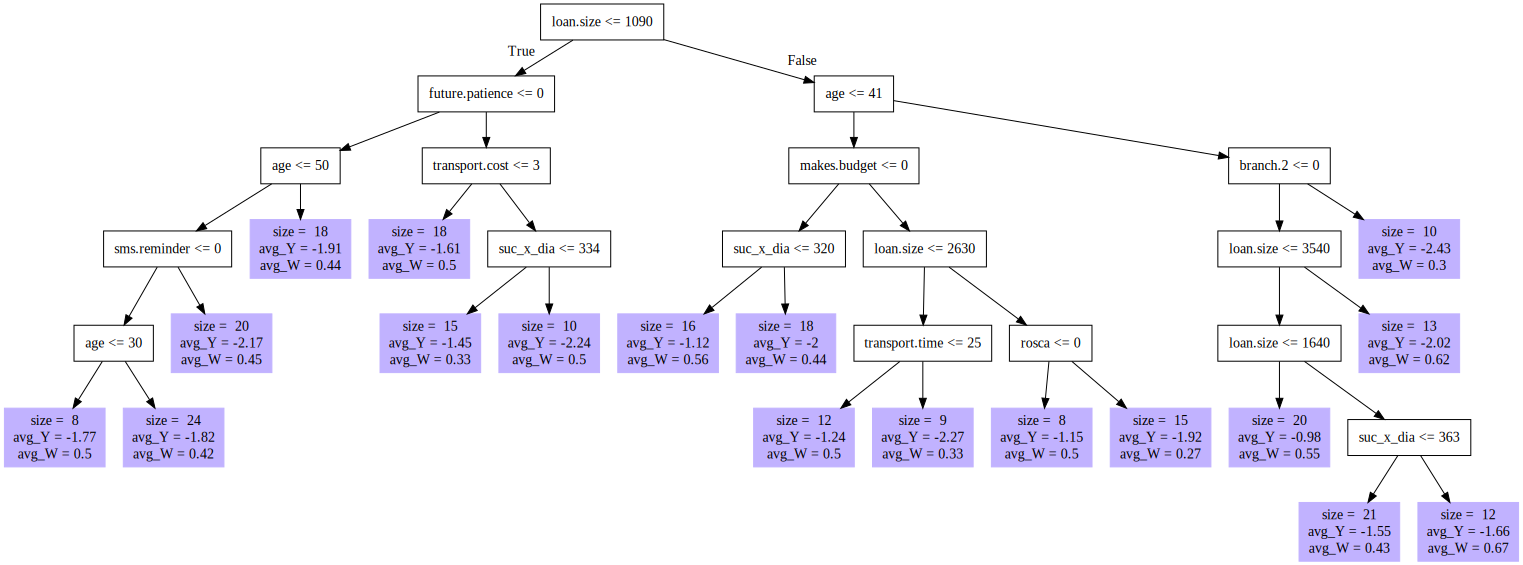
\includegraphics[width=\textwidth]{Figuras/crf_apr.pdf}
    \end{center}
    \legend{ 
    This figure shows an example of one of the regression trees used to compute the causal forest estimates described in Section \ref{sec:RF}. Each tree is constructed from a sequence of recursive binary partitions of the covariate space, with a splitting rule that is targeted to the causal quantity of interest, following the methodology of \cite{atheygrf}.}
    %This is one(it is chosen such that it minimizes the pruned cost, that is it is the tree with the smallest root-node impurity) of the honest causal trees in the random forest we use for the estimation of the heterogeneous treatment effect of the fee-forcing contract. It is meant only as an example of how these trees look like. The forest was such that there are as many estimated treatment effects as there are clients.
     %\footnotesize{ \textit{RScript: }  \texttt{grf.R}
\end{figure}


\begin{figure}[!htb]
    \begin{center}
  \caption{Cumulative Distribution Function of Conditional ATE Estimates}
  \includegraphics[width=0.7\textwidth]{Figuras/cdf_CATE.pdf} 
    \label{fig:CATEsurvival}
     \legend{This figure shows the share of borrowers who benefit from forced commitment, where ``benefit'' is defined as having an estimated conditional average treatment effect (ATE) above a specified threshold value. Results are based on the causal forest model from Section \ref{sec:RF}. The solid line equals $1 - F_\text{ATE}(\delta)$ where $F_\text{ATE}(\delta)$ denotes the CDF corresponding to the density of conditional ATE estimates from Figure \ref{heterogeneous_effects}. The blue shaded regions are associated 95\% confidence intervals. We estimate that at least 90\% of borrowers have a positive conditional ATE.}
    \end{center}
    
   
%\textit{Do file: }  \texttt{cdf_CATE.do}
\end{figure}
 


\begin{figure}[!htb]
    \caption{Conditional ATEs from ``wide'' and ``narrow'' covariate sets}
    \label{wide_narrow_forests}
    \begin{center}
    \begin{subfigure}{0.7\textwidth}
        \centering
        \includegraphics[width=\textwidth]{Figuras/scatter_hist_wide_narrow.pdf}
    \end{subfigure}
    \legend{This figure plots the relationship between the causal forest conditional ATE estimates from Section \ref{sec:RF} that use the ``wide'' set of covariates (all intake survey responses) and those based on a restricted ``narrow'' set of covariates (age, gender, HS education, and previous borrowing). The scatterplot graphs one estimate versus the other, with the ``wide'' covariate set on the horizontal axis and the ``narrow'' set on the vertical axis. The density plots on each axis show the estimated marginal distribution of conditional ATEs under each covariate set. The density for the ``wide'' covariate set is considerably more dispersed, as the causal forest based on this set of covariates captures considerably more treatment effect heterogeneity.}
    \end{center}
      

%\textit{Do file: } \texttt{wide_narrow_forests.do}       
\end{figure}







\subsection{Targeting rule comparisons}



\begin{figure}[!htb]
    \caption{Targeting rules}
    \label{targeting_rules}
    \begin{center}
    \begin{subfigure}{0.7\textwidth}
        \centering
        \includegraphics[width=\textwidth]{Figuras/wide_narrow_rule.pdf}
    \end{subfigure}
    \end{center}
      \legend{ This figure plots the percentage of borrowers who would benefit from a program in which commitment is targeted using the ``narrow'' covariate set (age, gender, HS education, and previous borrowing). In this exercise ``benefit'' is defined to mean having a conditional ATE above a particular threshold, taking the estimated conditional effects from the ``wide'' causal forest as ground truth. The plot compares the estimated percentage of borrowers who benefit, along with associated 95\% confidence bands, for three targeting rules: universal forced commitment in blue, targeting based on a random forest classification model in green, and targeting based on the logit model in red. For each of the classification models, the outcome variable is an indicator for whether the CATE estimate from the ``wide'' random forest model is positive. Each of the classification models produces an estimated probability of a positive CATE. For each, the assignment rule ranks borrowers by this estimated probability, and assigns the highest 90\% to forced commitment, to match the overall percentage of borrowers with positive estimated CATEs from the ``wide'' random forest model. Because this is an in-sample exercise, it overstates the actual performance of logit and RF-based targeting. }
     

\end{figure}


Figure \ref{targeting_rules} compares the in-sample performance of these targeting rules against a policy of universal forced commitment. The plot presents the estimated proportion of borrowers who benefit from a particular treatment assignment rule, along with associated 95\% confidence bands, where ``benefit'' is defined as having a conditional average treatment effect above a particular threshold. As above, we take the conditional average effects from the ``wide'' causal forest as ground truth for the purposes of this exercise. Because this is an in-sample exercise, the logistic and random forest classification rules have an unfair advantage: there is no adjustment for overfitting. In spite of this, their performance is quite unimpressive relative to a policy of universal forced commitment. The fraction of the whole sample incorrectly targeted when moving from universal forced commitment to targeting based on the narrow RF falls only from 9.78\% to 9.59\%. The logit targeting rule actually makes things marginally worse. 




\end{appendix}

\end{document}
